\chapter{Magnétostatique}
\label{chap:magnetostatique}
\section*{Objectifs}%
\label{sec:objectifs}
\begin{itemize}
	\item Connaître les équations qui contrôlent l'évolution spatiale 
	  du champ magnétostatique $\vecb$.
	\item Faire le lien entre ces équations et une carte de champ 
	  magnétique.
	\item Savoir calculer le champ magnétostatique résultant d'une 
	  distribution simple de courants.
\end{itemize}
\newpage
\section*{Introduction}
La magnétostatique étudie les champs magnétiques créés par des courants permanents.
Le plus souvent, on cherche alors à déterminer le champ magnétostatique $\vecb$
qui résulte d'une distribution de courant $\vecj$ connue. Nous nous intéressons
dans ce chapitre au champ magnétique créé par des courants circulants 
dans des conducteurs. Les milieux aimantés seront abordés plus loin dans le cours.

\section{La force de Lorentz}%
L'interaction entre deux particules immobiles a permis de définir la force de 
Coulomb dans le chapitre~\ref{chap:electrostatique}. Cette interaction 
électrostatique ne suffit plus lorsqu'il s'agit de décrire la dynamique de 
charges en mouvement. En 1895, le physicien néerlandais Hendrick Antoon Lorentz
propose alors l'ajout d'un second terme à la force coulombienne qui fait apparaître
la champ magnétostatique $\vecb$. 

\begin{defn}[Champ magnétostatique]
	Au même titre que le champ électrostatique, le champ magnétique $\vecb$
	est un champ vectoriel. Il est généré par une distribution de courant ou 
	par un aimant. Il s'exprime en tesla, noté $\tesla$ ($\kilogram \usk
	\rpsquare \second \reciprocal \ampere$ en SI). On rappelle quelques ordres de
	grandeur du champ magnétique
	
	\begin{center}
	\begin{tabular}{l|l}
		\textbf{Dispositif} 	& $\vecb (\tesla)$ \\ \hline
		Champ magnétique terrestre à la surface & $47 \times 10^{-6}$ \\
		Champ créé à $\unit{1}{\centi \meter}$ d'un fil parcouru par 
		un courant de $\unit{10}{\ampere}$
								 & $2 \times 10^{-5}$ \\
		Champ créé à $\unit{1}{\milli \meter}$ d'un aimant permanent& $0.1 - 1$ \\
		Électroaimant & $10 - 100$ \\
		Étoile à neutrons en surface & $10^{11}$\\
	\end{tabular}
	\end{center}
Le champ magnétique vérifie lui aussi le principe de superposition.
\end{defn}

\begin{defn}[Force de Lorentz]
Une particule de charge $q$ se déplaçant à la vitesse $\vecv$ dans un champ magnétique
$\vecb$, subit une force appelée force de Lorentz
\begin{equation}
	\vecf = q\vecv \wedge \vecb.
\end{equation}
Cette force est donc toujours orthogonale à la vitesse de la particule.
Contrairement à la force électrostatique, la force magnétique n'entraîne donc pas 
de variation de la vitesse de la particule, elle permet seulement de dévier sa 
trajectoire. En effet, la puissance magnétique $\mathcal{P}$ vaut
\begin{equation*}
	\mathcal{P} = \vecf \cdot \vecv = (q\vecv \wedge \vecb) \cdot \vecv = 0.
\end{equation*}
La force magnétique ne permet donc pas de mettre une particule chargée en mouvement.
\end{defn}

Comme pour la force électrostatique, le poids d'une particule chargée est bien souvent 
négligeable devant celui de la force de Lorentz. Pour illustrer cela, prenons le 
cas d'un électron de masse $m_e = \unit{9.1 \times 10^{-31}}{\kilogram}$ et de
charge $q = \unit{1.6 \times 10^{-19}}{\coulomb}$ se déplaçant à une vitesse
$v = \unit{10^5}{\meter \usk \reciprocal \second}$ dans un champ magnétique uniforme
$B = \unit{1}{\tesla}$. On trouve alors
\begin{equation*}
	\dfrac{mg}{qvB} \approx 10^{-15}.
\end{equation*}
On peut alors toujours négliger le poids d'une particule chargée
devant la force de Lorentz.

\begin{exemple}
	On s'intéresse ici au mouvement d'un électron de charge $-e$ et de 
	masse $m$ dans un 
	champ magnétique uniforme $\vecb$ (voir Fig.~\ref{fig:magneto_cyclotron}). 
	La vitesse initiale $\vecv_0$ de la particule est orthogonale au champ
	$\vecb$. La particule est donc soumise à la force de Lorentz et à son
	poids que nous négligeons ici. 
	
	Expérimentalement, on constate que la trajectoire 
	de la particule est circulaire. La force de Lorentz ne travaillant pas, 
	la norme de la vitesse reste en tout temps égale à $v_0$. Le mouvement de la 
	particule est donc uniforme et circulaire.
	
	On se place dans
	un référentiel polaire $(O, \er, \etheta)$. La position de la particule
	est donc repérée par ses coordonnées $(r, \theta)$. L'application du principe
	fondamental de la dynamique à la particule dans le référentiel du
	laboratoire supposé galiléen donne
	\begin{equation*}
		m \dot{\vecv} = q \vecv \wedge \vecb,
	\end{equation*}
	où la notation $\dot{v}$ est utilisée pour la dérivée temporelle.
	Dans un référentiel polaire et pour un mouvement circulaire uniforme, 
	$\vecv = r\dot{\theta} \etheta = v_0 \etheta$ 
	et $\dot{\vecv} = - v_0^2/r\er$. On obtient donc
	\begin{equation*}
		m \dfrac{v_0^2}{r}\er = -e v_0 \etheta \wedge \ez =e v_0 B \er \iff 
		\dot{\theta} = \dfrac{eB}{m}
	\end{equation*}
	L'électron suit donc un mouvement circulaire uniforme à la vitesse angulaire
	$eB/m$ appelée pulsation cyclotron. Dans le cyclotron de University of Michigan,
	le champ magnétique vaut $B = \unit{0.10}{\tesla}$, ce qui donne une pulsation de 
	$\unit{1.7 \times 10^{10}}{\rad \usk \reciprocal \second}$ pour un électron.

\end{exemple}
\begin{figure}[h!]
	\centering
	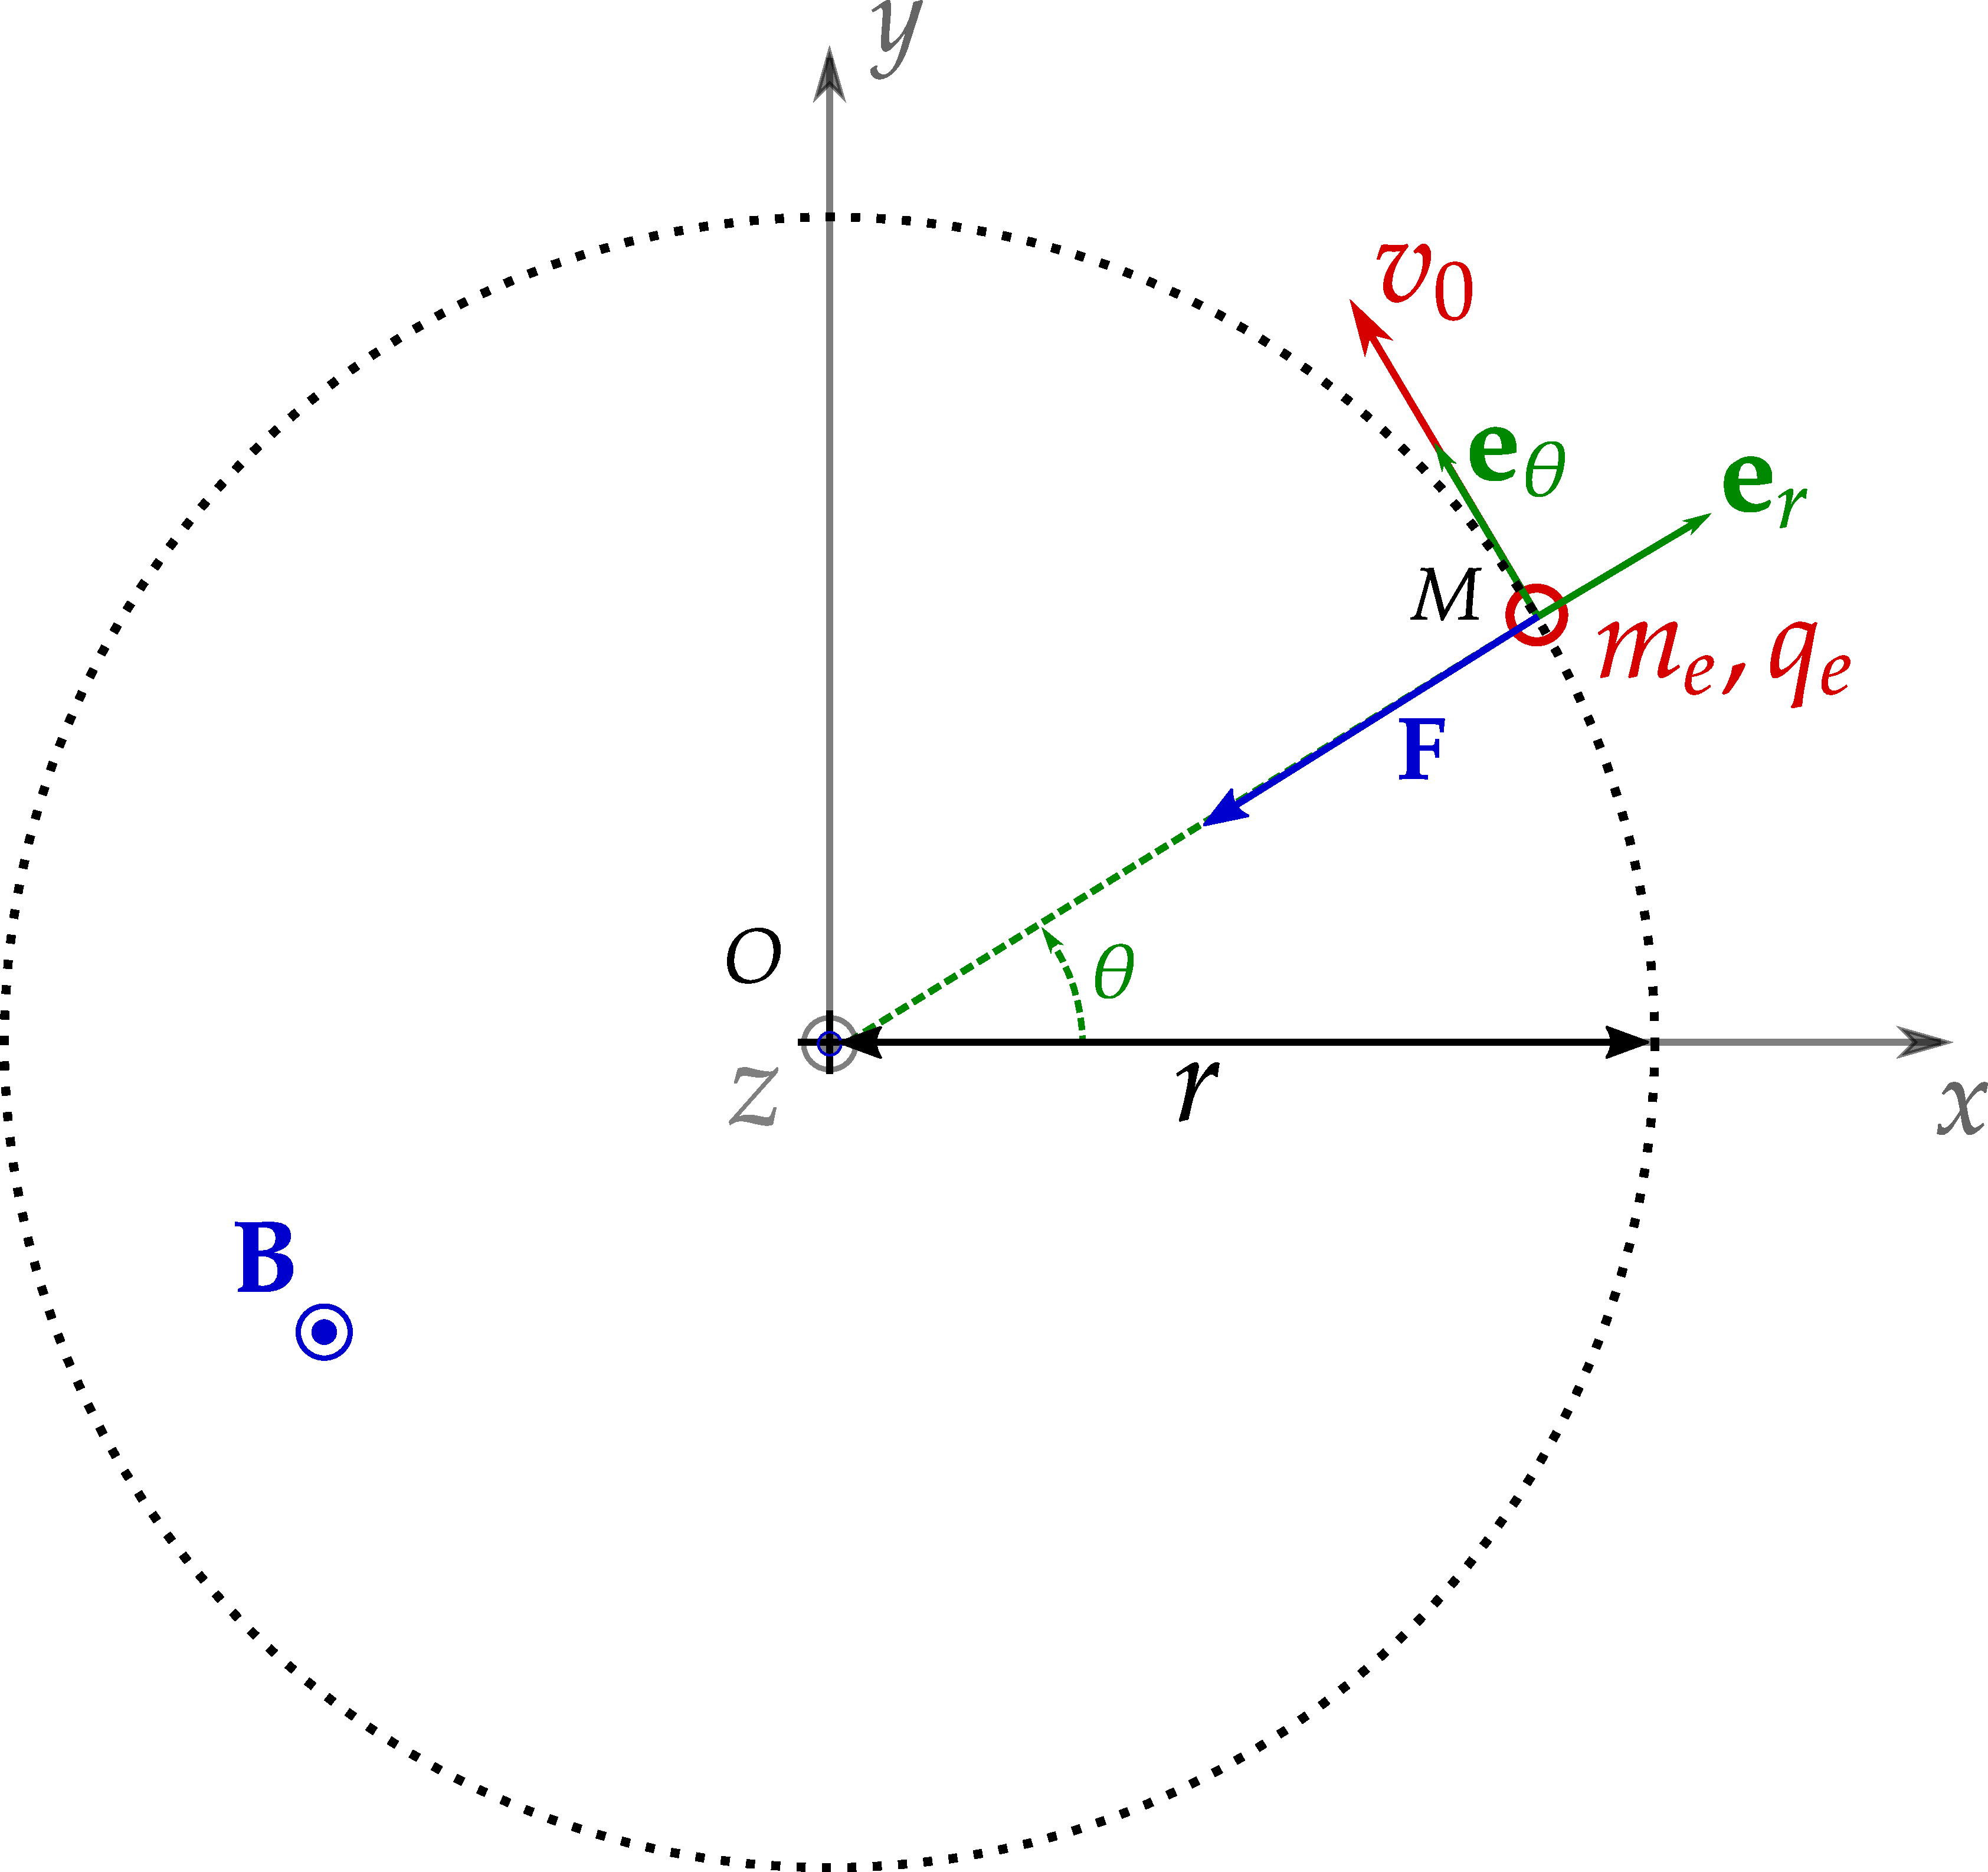
\includegraphics[scale=0.75]{cyclotron}
	\caption{Trajectoire d'un électron dans un champ magnétique uniforme.}%
	\label{fig:magneto_cyclotron}
\end{figure}

\section{La loi de Biot et Savart}
De la même manière que pour le champ électrostatique, nous
commençons par définir le champ magnétique généré par une charge ponctuelle. 
Soit une charge ponctuelle $q$ en un point $P$ de l'espace se déplaçant 
à la vitesse $\vecv$ dans le référentiel du laboratoire. Expérimentalement,
on observe que cette particule génère
en un point $M$ un champ magnétique $\vecb(M)$ tel que

\begin{equation*}
	\vecb(M) = \dfrac{\mu_0 q}{4 \pi} \vecv \wedge \dfrac{\mitbf{PM}}{||PM||^3},
\end{equation*}
où $\mu_0 = \unit{4 \pi \times 10^{-7}}{\tesla \usk \meter \usk \reciprocal 
\ampere}.$

\begin{figure}[h!]
	\centering
	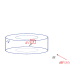
\includegraphics[]{biot_savart}
	\caption{Champ magnétique généré par un élément infinitésimal d'un conducteur
	de densité volumique de courant $\vecj$ en un point $M$ de l'espace.}%
	\label{fig:magneto_biot_savart}
\end{figure}

On considère un conducteur formant un volume $\mathcal{V}$ 
(voir Fig.~\ref{fig:magneto_biot_savart}) parcouru par des charges mobiles 
de densité volumique de charge $\rho$ se déplaçant à la vitesse $\vecv$. Un élément 
infinitésimal $\dV$ de ce circuit centré en $P$ génère en un point $M$ un champ magnétique

\begin{equation*}
	\mathrm{\textbf{d}}\mitbf{B}^P(M) = \dfrac{\mu_0 \rho(P) \dV}
	{4 \pi} \vecv(P) \wedge 
	          \dfrac{\mitbf{PM}}{||PM||^3},
\end{equation*}
où on reconnaît le vecteur densité de courant $\vecj(P) = \rho(P) \vecv(P)$. 
Le champ magnétique
$\vecb$ généré par l'ensemble du circuit en $M$ est alors obtenu en additionnant les 
contributions de chaque élément de ce dernier grâce au principe de superposition
\begin{equation*}
	\vecb(M) = \iiint_{P \in \mathcal{V}} \mathrm{\textbf{d}}\mitbf{B}^P(M)
		 = \iiint_{P \in \mathcal{V}} \dfrac{\mu_0}
		 {4 \pi} \vecj(P) \wedge 
	          \dfrac{\mitbf{PM}}{||PM||^3} \dV
\end{equation*}
On aboutit ainsi à la loi de Biot et Savart.

\begin{defn}[Loi de Biot et Savart]
	Le champ magnétostatique $\vecb(M)$ créé au point $M$ par une distribution
	volumique de courant $\vecj$ ($\ampere \usk \rpsquare \meter$) contenue
	dans un volume $\mathcal{V}$ est
	\begin{equation}
		\vecb(M) = \dfrac{\mu_0}{4 \pi} \iiint_{P \in \mathcal{V}} 
		\dfrac{\vecj(P) \wedge \mitbf{PM}}{||PM||^3} \dV,
	\end{equation}
	où $\mu_0 = \unit{4 \pi \times 10^{-7}}{\tesla \usk \meter \usk \reciprocal
	\ampere}$ est la perméabilité magnétique du vide.

\end{defn}

	Par un raisonnement similaire, on montre que pour une distribution 
	surfacique de courant $\vecj_s$ confinée sur une 
	surface $\mathcal{S}$, cette expression devient
	\begin{equation}
		\vecb(M) = \dfrac{\mu_0}{4 \pi} \iint_{P \in \mathcal{S}} 
		\dfrac{\vecj_s(P) \wedge \mitbf{PM}}{||PM||^3} \mathrm{d}S.
	\end{equation}

	Pour un circuit filiforme $\mathcal{C}$ parcouru par un courant $I$, 
	cette expression devient
	\begin{equation}
		\vecb(M) = \dfrac{\mu_0}{4 \pi} \int_{P \in \mathcal{C}} 
	\dfrac{I \dl \wedge \mitbf{PM}}{||PM||^3}.
	\end{equation}

\begin{exemple}
	On cherche à déterminer le champ magnétique généré par un fil infini $\mathcal{C}$
	parcouru
	par un courant d'intensité $I$ en un point $M$ 
	(voir Fig.~\ref{fig:magneto_spire}). On se place dans un repère cylindrique
	$(0, \er, \etheta, \ez)$. Les points $M$ et $P$ ont pour coordonnées 
	respectives $(r, \theta, 0)$ et $(0, 0, z_P)$.

	Le champ magnétique $\mathrm{\textbf{d}}\vecb^P(M)$ généré par un élément
	$\dl_P$ du fil centré en $P$ s'écrit
	\begin{equation*}
	\mathrm{\textbf{d}}\vecb^P(M) = \dfrac{\mu_0}{4 \pi} 
	              \dfrac{I \dl_P \wedge \mitbf{PM}}{||PM||^3},
	\end{equation*}
	où $\mitbf{PM} = \mitbf{PO} + \mitbf{OM} = - z_P\ez + r\er$. Dans un repère
	cylindrique, un élément infinitésimal $\dl_P$ du fil s'écrit
	$\dl_P = \dz_P \ez$. On a alors
	\begin{equation*}
		\dfrac{\dl_P \wedge \mitbf{PM}}{||PM||^3} = 
		\dfrac{r\dz_P}{||PM||^3}\etheta. 	
	\end{equation*}
	En remarquant que $||PM|| = r/\cos\alpha$, l'expression précédente devient alors
	\begin{equation*}
		\dfrac{r\dz_P}{||PM||^3}\etheta = \dfrac{\cos^3\alpha \dz_P}
		{r^2} \etheta
	\end{equation*}
	De même, on remarque que $z_p = r \tan\alpha$.
	Par différentiation, on obtient donc
	\begin{equation*}
		\dz_P = \mathrm{d}\left[r\tan\alpha\right] = 
		\dfrac{r \mathrm{d}\alpha}{\cos^2\alpha}.
	\end{equation*}
	Finalement,
	\begin{equation*}
		\mathrm{\textbf{d}}\vecb^P(M) = \dfrac{\mu_0 I \cos\alpha}
		{4 \pi r} \mathrm{d}\alpha \etheta.
	\end{equation*}
	Le champ $\vecb(M)$ généré au point $M$ par le fil s'obtient alors
	en utilisant le principe de superposition, ce qui revient à intégrer les champs 
	magnétiques infinitésimaux sur l'ensemble du fil. Pour parcourir l'ensemble du
	fil, $\alpha$ doit varier entre $-\pi/2$ et $\pi/2$. On a alors
	\begin{equation*}
		\boxed{\vecb(M) = \dfrac{\mu_0 I}{4\pi r}
			\times \displaystyle{\int_{-\pi/2}^{\pi/2} 
			\cos\alpha\mathrm{d}\alpha \etheta} =
	\dfrac{\mu_0 I}{2\pi r}\etheta.}
	\end{equation*}
	On obtient un champ magnétique porté par $\etheta$ et donc la norme ne dépend
	que de $r$. Les lignes de ce champ sont des cercles concentriques centrés
	sur le fil. $\vecb$ "tourne" autour du fil.
\end{exemple}
\begin{figure}[h!]
	\centering
	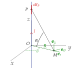
\includegraphics[scale=0.7]{fil}
	\caption{Champ magnétique créé en un point $M$ par un fil parcouru par
	un courant d'intensité $I$.}%
	\label{fig:magneto_spire}
\end{figure}

\begin{defn}[Calcul du champ magnétique par la loi de Biot et Savart]
	Comme nous l'avons vu dans l'exemple précédent, la loi de Biot et Savart
	peut s'avérer utile lorsqu'il s'agit de calculer le champ magnétique 
	$\vecb$ généré par une distribution de courant. Voici en résumé la démarche à suivre
	\begin{enumerate}
		\item Réaliser un schéma du système et choisir un repère adapaté.
		\item Exprimer le petit volume $\dV$, de surface $\mathrm{d}S$
		  ou de longueur $\dl$ dans ce système de coordonnées.
	  \item En multipliant cet élément par le courant ($\vecj$, $\vecj_s$ ou
	    $I$), on obtient le petit élément de courant associé.
	  \item Exprimer le vecteur $\mitbf{PM}$ dans le système de coordonnées
	    choisi.
    	\item En multipliant par $\dfrac{\mu_0}{4 \pi}$ et en faisant le produit 
	  vectoriel par $\dfrac{\mitbf{PM}}{||PM||^3}$, on fabrique le champ
	  élémentaire $\mathrm{\textbf{d}}\vecb^P(M)$ généré en $M$.
	\item Pour calculer $\vecb(M)$, il suffit alors d'intégrer sur la distribution
	  de courant.
	\end{enumerate}
\end{defn}
\section{Équation de la magnétostatique}
On considère un fil parcouru par un courant $I$ dans un
repère cylindrique $(O, \er, \etheta, \ez)$ (voir Fig.~\ref{fig:magneto_spire}). 
Comme vu ci-dessus, le champ
magnétique créé par ce fil en un point $M$ situé à une distance $r$ du fil
est donné par
\begin{equation*}
	\vecb(M) = \dfrac{\mu_0 I}{2 \pi r}\etheta.
\end{equation*}
Comme pour le champ électrostatique, nous allons nous servir de cet exemple simple 
pour retrouver certaines propriétés du champ magnétostatique.

\subsection{Le théorème d'Ampère}
Le théorème d'Ampère est l'équivalent pour le champ magnétostatique $\vecb$
du théorème de Gauss. Il va nous permettre de calculer facilement le champ
magnétostatique généré par une distribution de courants simple.

Les lignes du champ $\vecb$ créé par le fil sont des cercles dont l'axe est le
fil. Nous cherchons donc dans un premier temps à calculer la circulation de $\vecb$ 
sur la ligne de champ $\mathcal{C}$ de rayon $r$ passant par $M$. 
On a bien pris soin au préalable
d'orienter cette dernière. Dans un repère cylindrique, un petit élément $\dl$ de ce 
contour fermé s'écrit $\dl = r \dtheta \etheta$. La circulation de $\vecb$ sur
ce contour s'écrit donc
\begin{equation*}
	\boxed{\displaystyle{\oint_\mathcal{C} \vecb \cdot \dl = 
		\oint_0^{2 \pi} \dfrac{\mu_0 I}{2 \pi r} r\dtheta
	= \mu_0 I.}}
\end{equation*}
On constate que la circulation du champ $\vecb$ le long du circuit $\mathcal{C}$
ne dépend que du courant $I$ que ce dernier enlace. Cette propriété que nous venons
de montrer pour un fil est en fait une propriété générale du champ magnétostatique.

\begin{defn}[Théorème d'Ampère]
	La circulation du champ magnétostatique $\vecb$ le long d'un circuit fermé
	$\mathcal{C}$ est égale au courant \textbf{algébrique} $I_\mathrm{int}$ 
	enlacé par ce dernier multiplié
	par $\mu_0$
	\begin{equation}
		\oint_\mathcal{C} \vecb \cdot \dl = \mu_0 I_\mathrm{int}.
	\end{equation}
	Le contour sur lequel est réalisée l'intégrale est appelé contour d'Ampère.
	Le courant enlacé $I_\mathrm{int}$ est le courant qui traverse une surface 
	orientée
	qui s'appuie sur le contour d'Ampère. L'orientation de la surface 
	se déduit de celle du contour
	grâce à la règle de la main droite ou du tire-bouchon.
\end{defn}

\begin{exemple}
	\begin{minipage}{0.6\linewidth}
	Soit deux fils électriques parcourus par des courants $I_1$ et $I_2$.
	Avec les orientations choisies, le théorème d'Ampère appliqué au 
	contour $\mathcal{C}$ s'écrit
	\begin{equation*}
		\oint_\mathcal{C} \vecb \cdot \dl = \mu_0(I_1 - I_2).
	\end{equation*}
	\end{minipage}
	\hfill
	\begin{minipage}{0.35\linewidth}
		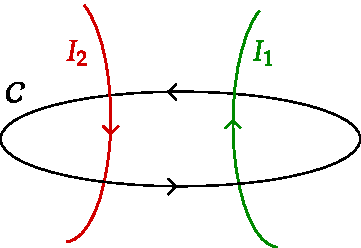
\includegraphics[width=0.8\linewidth]{ampere_ex}
	\end{minipage}

\end{exemple}

Le théorème d'Ampère peut-être traduit sous une forme locale:
appelée \textbf{équation de Maxwell-Ampère}, qui relie alors le champ magnétostatique
au vecteur densité de courant.

\begin{defn}[Équation de Maxwell-Ampère]
	L'équation de Maxwell-Ampère relie le champ magnétostatique $\vecb$
	au vecteur densité de courant $\vecj$
	\begin{equation}
		\rot \vecb = \mu_0 \vecj.
		\label{eq:magneto_ma}
	\end{equation}
	Cette équation est une relation $\textbf{locale}$, elle permet de relier 
	les dérivées spatiales du champ $\vecb$ en un point de l'espace au vecteur
	$\vecj$ en ce même point.
\end{defn}

\subsection{Flux du champ magnétostatique $\vecb$}
On cherche maintenant à calculer la divergence du champ $\vecb$. En coordonnées 
cylindriques, cela donne
\begin{equation*}
	\div \vecb = \dfrac{1}{r}\left(\dd{r B_r}{r} + \dd{B_\theta}{\theta} \right)
	+ \dd{B_z}{z},
\end{equation*}
où $B_r$, $B_\theta$ et $B_z$ sont les composantes de $\vecb$. 
Dans le cas du fil infini, $B_\theta$ est la seule composante non nulle de $\vecb$ 
et elle ne dépend pas
de $\theta$. On a donc
\begin{equation*}
	\div \vecb = 0.
\end{equation*}
Ce résultat se généralise à un champ magnétostatique $\vecb$ quelconque sous
la forme de l'équation de Maxwell-Thomson.

\begin{defn}[Équation de Maxwell-Thomson]
	Un champ magnétique $\vecb$ vérifie toujours
	\begin{equation*}
		\div \vecb = 0.
	\end{equation*}
	Cette relation locale est vérifiée en tout point de l'espace.
\end{defn}

\begin{rem}
La divergence de $\vecb$ étant nulle, l'analyse vectorielle affirme
qu'il est possible dans ce cas de définir un champ vectoriel $\veca$,
défini à un gradient près, tel que $\rot \veca = \vecb$,
appelé le potentiel vecteur.
\end{rem}

Comme l'équation de Maxwell-Ampère, cette équation peut se mettre sous une forme
intégrale, en exprimant le flux du champ magnétique à travers une surface fermée
$\mathcal{S}$.

\begin{defn}[Flux du champ magnétostatique]
	Le flux du champ magnétique $\vecb$ à travers une surface fermée 
	$\mathcal{S}$ est nul
	\begin{equation*}
		\oiint_\mathcal{S} \vecb \cdot \ds = 0.
	\end{equation*}
	On dit que le champ $\vecb$ est à flux conservatif.
\end{defn}

	\begin{minipage}{0.6\linewidth}
	On peut appliquer ce résultat à une surface $\mathcal{S}$ particulière
	constituée d'une portion de tube de champ de section d'entrée $\mathcal{S}_e$,
	de section de sortie $\mathcal{S}_s$ et de section latérale $
	\mathcal{S}_l$. 	
	\end{minipage}
	\hfill
	\begin{minipage}{0.3\linewidth}
	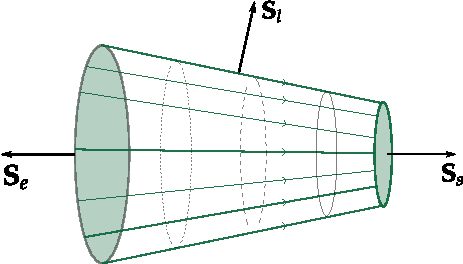
\includegraphics[scale=0.7]{tube}
	\end{minipage}
	\vspace{0.5cm}

\begin{defn}[Tube de champ]
	L'ensemble des lignes de champ s'appuyant sur un contour fermé forme un 
	tube de champ.
\end{defn}
	
	D'après le théorème d'Ampère la flux de $\vecb$ à
	travers cette surface est nul.
	Par définition du tube de champ, l'intégrale sur la surface 
	latérale est nulle. Il reste donc 
	\begin{equation*}
		\iint_\mathcal{S_e} \vecb \cdot \ds_e =
		- \iint_\mathcal{S_s} \vecb \cdot \ds_s 
		\iff
		\displaystyle{\left\lvert\iint_\mathcal{S_e} \vecb \cdot \ds_e\right\rvert =
		\left\lvert\iint_\mathcal{S_s} \vecb \cdot \ds_s\right\rvert}.
	\end{equation*}
	Le flux entrant dans la surface est égal au flux sortant de cette dernière.
	De plus, la surface de sortie étant de taille plus importante que 
	la surface d'entrée, on en conclut que le champ est plus intense
	à l'entrée du tube qu'à la sortie. Le champ $\vecb$ étant à flux
	conservatif, un resserrement des lignes de champs traduit une augmentation
	de l'intensité de ce dernier.

\begin{defn}[Flux conservatif et lignes de champ]
	Le champ magnétique étant à flux conservatif, ses lignes de champs
	se resserrent dans les zones de forte intensité. Inversement, ces dernières
	s'éloignent lorsqu'il devient plus faible
\end{defn}

\section{Étude des lignes de champ de \vecb}
Nous nous intéressons dans cette partie aux propriétés spatiales du champ $\vecb$.
Nous allons voir comment les \textbf{lignes de champ} nous renseignent sur sa répartition 
dans l'espace.

Nous nous intéressons au champ magnétique produit par un solénoïde 
(voir Fig.~\ref{fig:magneto_solenoide}).
Les lignes de champ nous permettent de retrouver quelques propriétés du champ 
magnétostatique énoncées précédemment.

\begin{figure}[htpb]
	\centering
	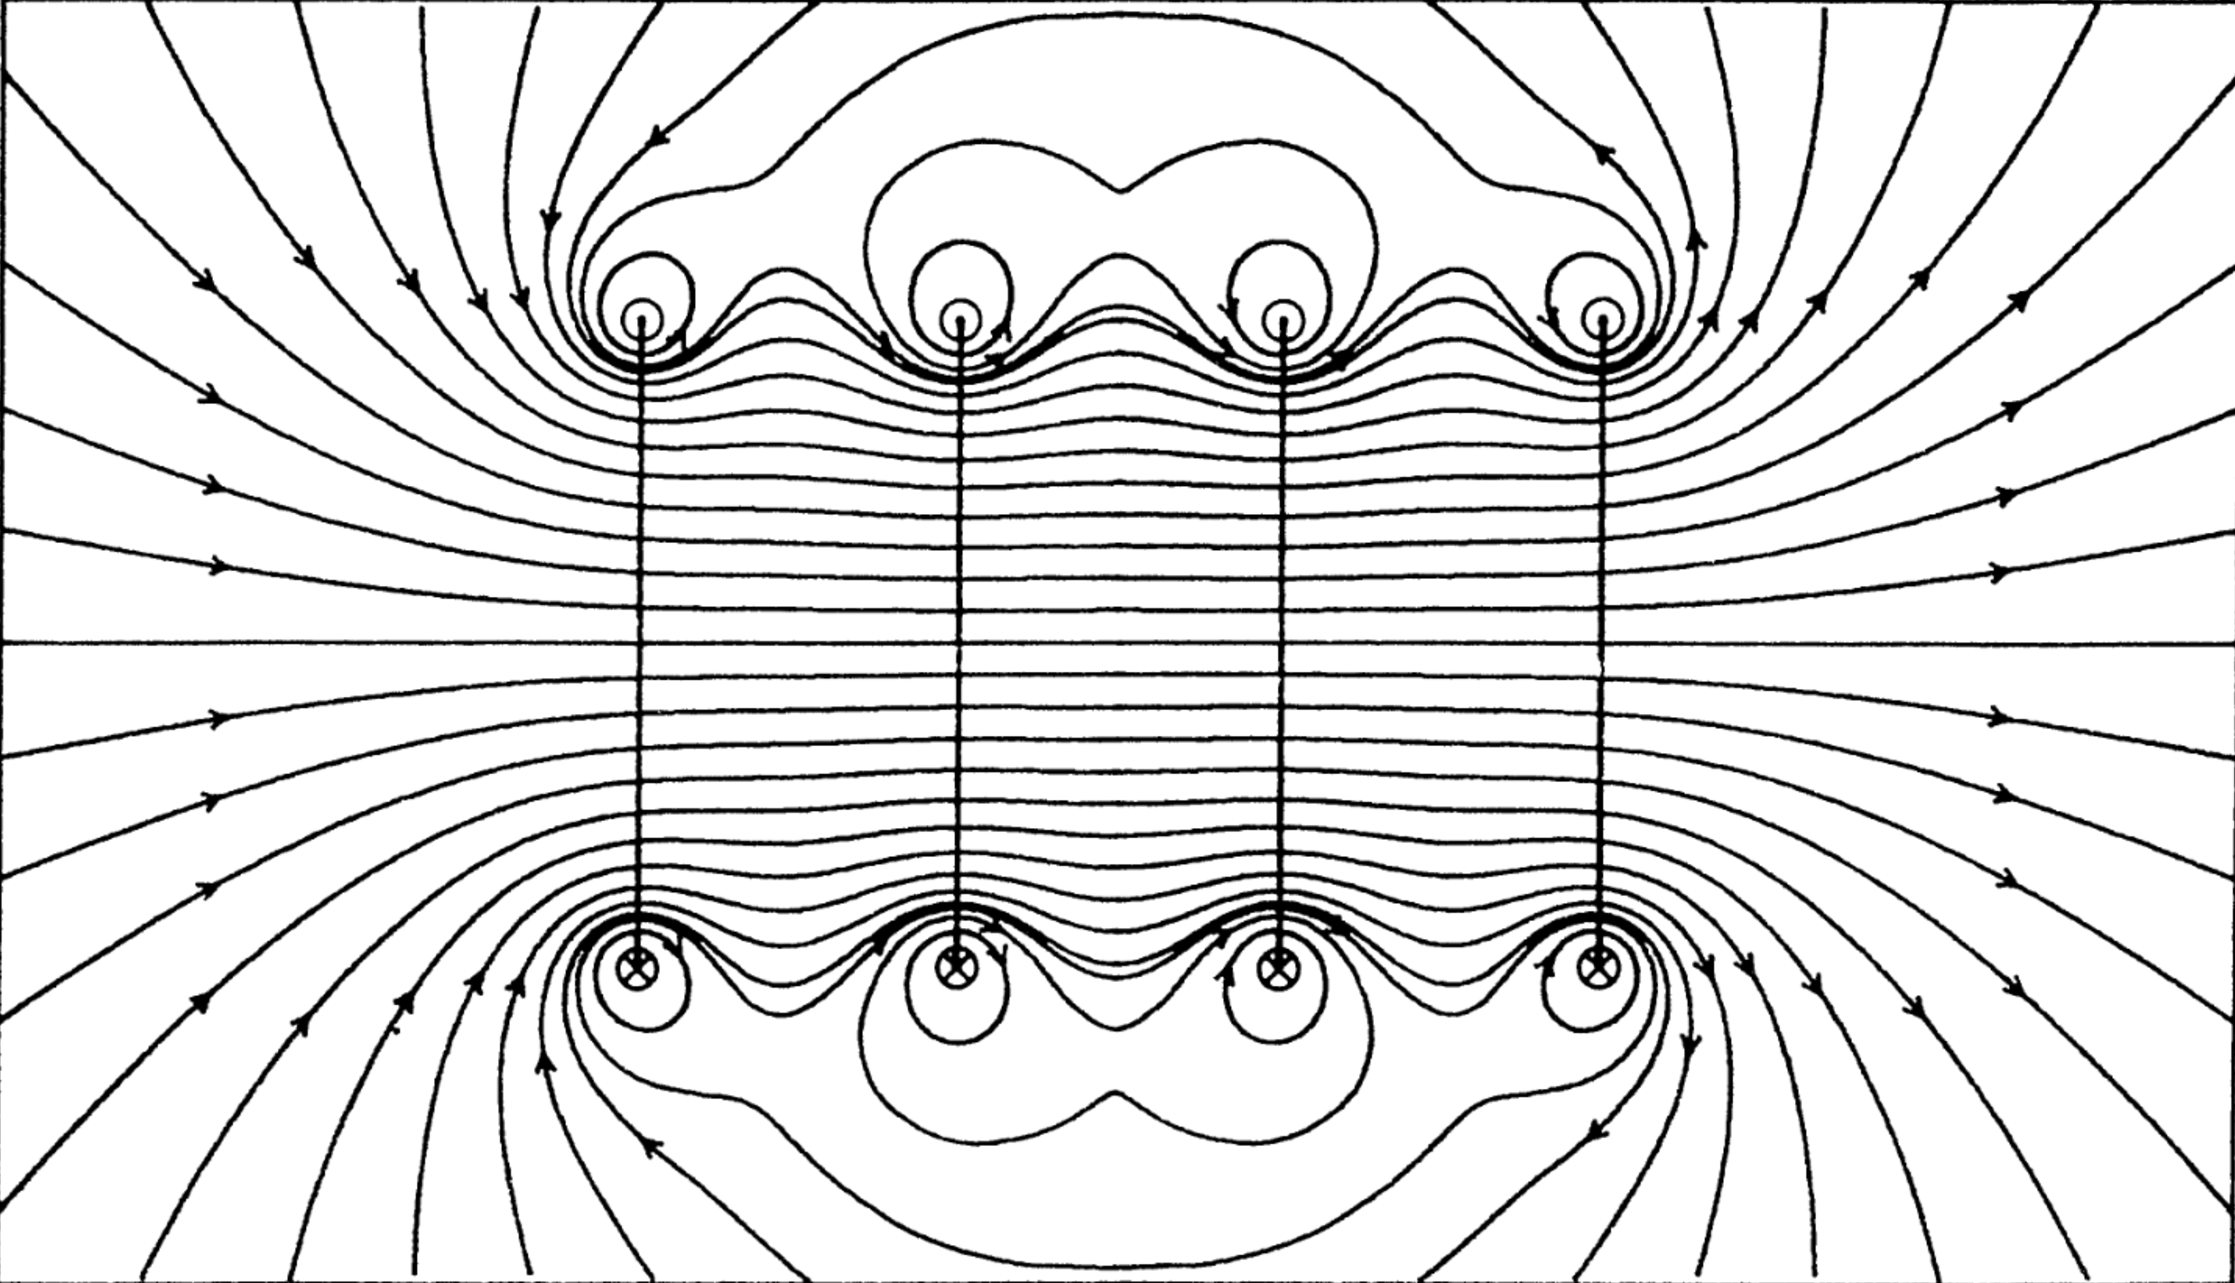
\includegraphics[width=0.7\linewidth]{solenoide}
	\caption{Lignes du champ magnétique généré par un solénoïde constitué de
		4 bobines parcourues dans le même sens par la même intensité.
		Cette figure est extraite de \cite{Gie1985}}%
	\label{fig:magneto_solenoide}
\end{figure}

\begin{enumerate}
	\item On remarque tout d'abord que les lignes de champ 
	  sont des contours fermés qui entourent les fils parcourus par un courant.
	  Cette première observation est une conséquence directe de l'équation
	  de Maxwell-Ampère. L'orientation de ces lignes de champ s'obtient
	  d'ailleurs en considérant le sens du courant dans les fils et en utilisant
	  la règle de la main droite.
      \item La divergence nulle de $\vecb$ est aussi visible sur cette carte de 
	champ. En effet, on constate que les lignes de champ ne convergent/divergent
	pas en un point de l'espace, contrairement au champ électrostatique.
      \item Dans le cas du champ magnétique, le resserrement des lignes de champ
	traduit une augmentation de la norme de ce dernier. On conclut que le champ
	est plus intense à l'intérieur du solénoïde qu'à l'extérieur. De plus, les
	lignes de champ étant parallèles à l'intérieur du solénoïde, on conclut que
	le champ est uniforme.
      \item Grâce aux lignes de champ, on retrouve rapidement les plans de 
	  symétrie et d'antisymétrie du champ magnétique. Le plan médiateur 
	  du solénoïde est par exemple un plan de symétrie du champ magnétique. 
          L'analyse de ces symétries sera utile pour calculer le champ
          magnétique résultant d'une distribution de courant.
\end{enumerate}

\section{Calcul du champ magnétostatique}
\label{sec:calcul_e}
Nous allons voir dans cette partie comment nous pouvons utiliser le théorème d'Ampère
pour calculer le champ magnétostatique $\vecb$ créé 
par une distribution de courants simple. Nous nous intéressons ici à une bobine
torique constituée d'un fil régulièrement bobiné autour d'un tore de section
carré (voir Fig.~\ref{fig:magneto_tore}). Cette bobine est caractérisée par le nombre $N$
total de spires bobinés, son rayon intérieur $R$ 
et sa hauteur $h$. La bobine est parcourue par un courant $I$.

On cherche à déterminer 
l'expression du champ électrique $\vecb$ en un point $M$ de l'espace. Pour ce faire, 
il suffit de suivre le mode d'emploi suivant
\begin{enumerate}
	\item Faire un schéma du système ! C'est absolument indispensable
	  (voir Fig.~\ref{fig:magneto_tore})
	\item Choisir un repère adapté au problème
	\item Étudier les invariances de cette distribution
	\item Étudier les symétries de la distribution de courants à l'origine 
	  du champ magnétostatique
	\item Choisir un contour d'Ampère et appliquer le théorème d'Ampère.
\end{enumerate}

Au vu de la géométrie du système, nous choisissons ici d'utiliser 
un repère cylindrique $(O, \er, \etheta, \ez)$.
Le point $M$ est donc repéré par ses coordonnées $(r, \theta, z)$. Le champ
magnétostatique en $M$ s'écrit de manière générale

\begin{equation}
	\vecb(M) = B_r(M)\er + B_\theta(M)\etheta + B_\varphi(M)\ephi.
	\label{eq:tore}
\end{equation}
Le champ magnétostatique est un vecteur à trois composantes et chaque composante
dépend des coordonnées de $M$. Pour simplifier cette expression, il est intéressant
de considérer les invariances et symétries de la distribution de courant qui génère
le champ $\vecb$.

\begin{figure}
	\centering
	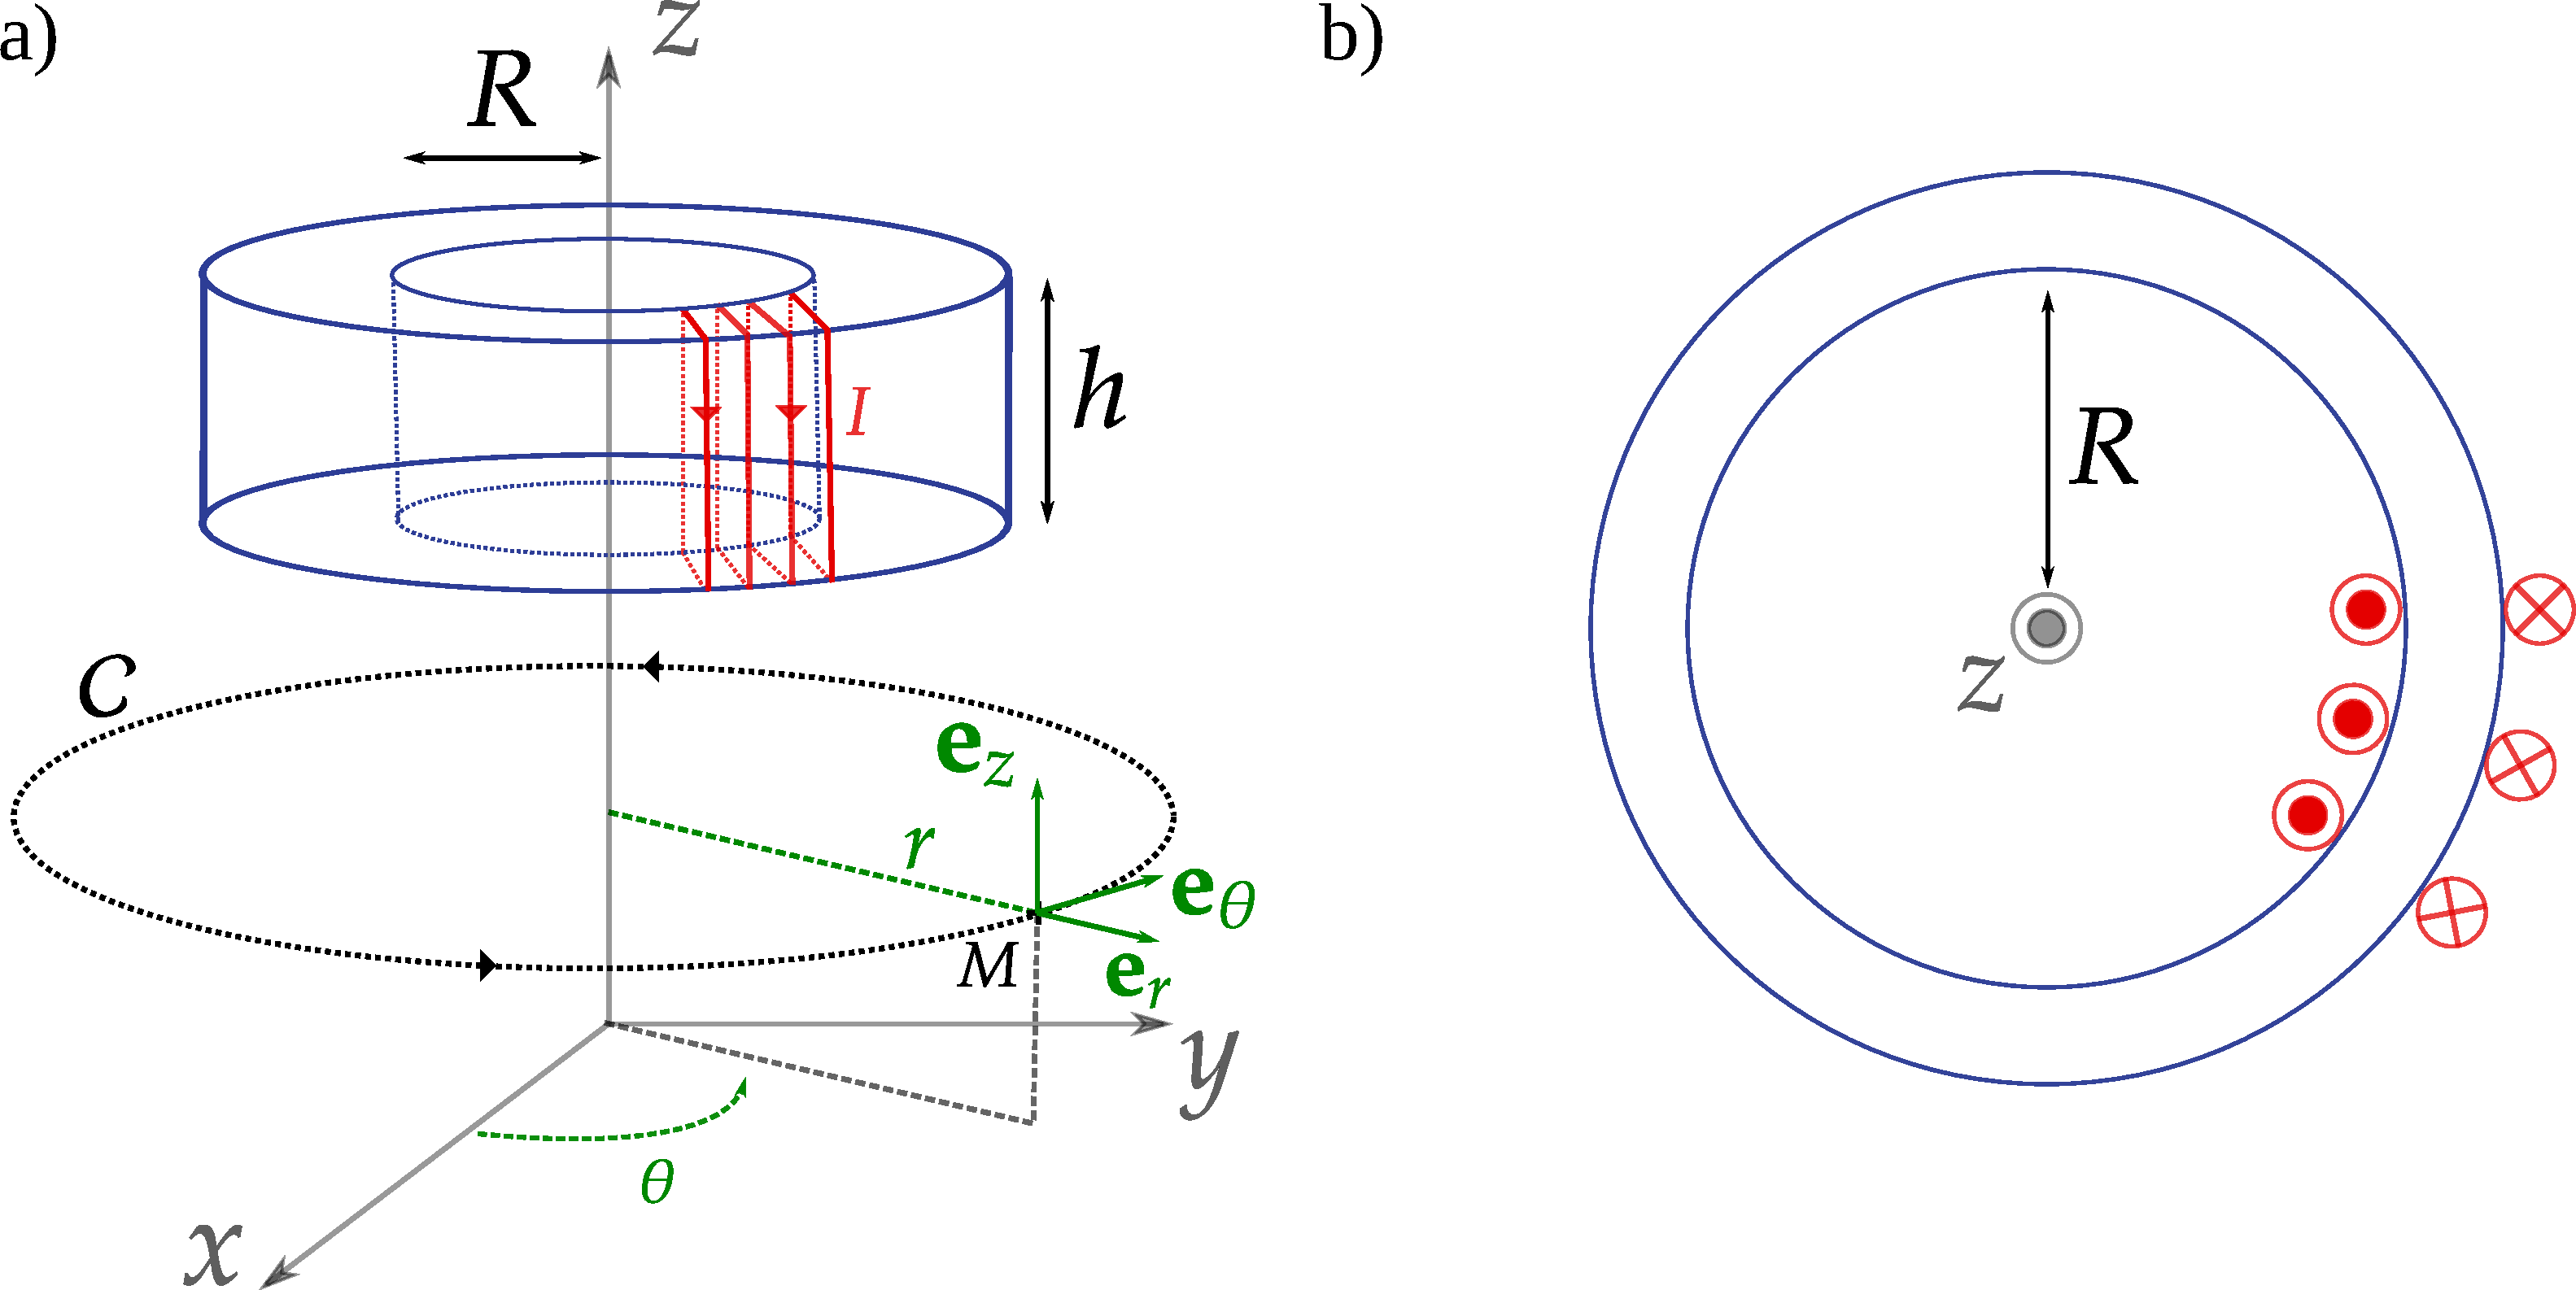
\includegraphics[scale=1]{tore}
	\caption{Bobine torique à gauche et coupe perpendiculaire à $(Oz)$
	de cette bobine à droite.}%
	\label{fig:magneto_tore}
\end{figure}

\subsection{Invariance de la distribution de courants}
On cherche ici à savoir si la distribution de courant est modifiée sous l'effet
d'une translation ou d'une rotation de l'espace. En d'autres termes, on regarde
de quelles variables elle dépend. Étant donné que les spires sont uniformément
répartie sur le tore, on observe que

\begin{itemize}
	\item  si je tourne le tore d'un angle $\Delta \theta$ dans la
	  direction $\etheta$, le problème
	  ne change pas. La distribution de courant est donc invariante 
	  par rotation selon l'angle $\theta$. $\vecb$ \textbf{ne dépend pas de
	  $\mitbf{\theta}$}.
\end{itemize}

Finalement, l'expression~\ref{eq:tore} du champ magnétique se simplifie donc en 

\begin{equation*}
	\boxed{\vecb(M) = B_r(r,z)\er + B_\theta(r,z)\etheta + B_z(r,z)\ez.}
\end{equation*}
\subsection{Symétries de la distribution de courants}

Si on applique ce principe au champ magnétique créé par une distribution 
de courants, cela revient à dire que les symétries de la distributions de 
courants doivent se retrouver dans les symétries du champ magnétique. On en 
déduit les règles suivantes

\begin{defn}[Symétries de $\vecb$ et de la distribution de courant]
\begin{itemize}
  \item si $(\Pi)$ est un plan d'antisymétrie de la distribution de courant et que 
    $M$ appartient à $(\Pi)$, alors obligatoirement $\vecb(M)$ doit 
    appartenir à $(\Pi)$,
  \item si $(\Pi)$ est un plan de symétrie de la distribution de courant 
    et que $M$ appartient à $(\Pi)$, alors obligatoirement $\vecb(M)$ doit 
    être orthogonal à $(\Pi)$.
\end{itemize}
\end{defn}

\begin{rem}
	Le champ magnétostatique $\vecb$ appartient aux plans d'\textbf{antisymétrie}
	de la distribution de courant et non aux plans de symétrie comme
	c'est le cas pour le champ électrostatique. Le vecteur $\vecb$ est 
	qualifié de vecteur axial.
\end{rem}

Pour appliquer ces règles à notre exemple, on détermine les plans de symétrie 
et d'antisymétrie de la distribution de courants auquels 
le point $M$ appartient

\begin{itemize}
	\item le plan $(M, \er, \ez)$ est un plan de symétrie de la distribution
	  de courant. $\vecb(M)$ \textbf{doit être orthogonal à ce plan}.
\end{itemize}

$\vecb(M)$ doit être orthogonal au plan $(M, \er, \ez)$, 
il doit donc être colinéaire à $\etheta$

\begin{framed}
\begin{equation*}
	\vecb(M) = B_\theta(r, z) \etheta.
\end{equation*}
\end{framed}

Nous n'avons imposé aucune condition sur la position de $M$, cette relation est
donc vraie pour tout point $M$ de l'espace. Maintenant que l'expression du 
champ magnétique a été simplifiée au maximum, on cherche à appliquer le théorème
d'Ampère.

\subsection{Application du théorème d'Ampère}
La distribution de courant présente une symétrie de révolution. On choisit comme contour 
d'Ampère un cercle $\mathcal{C}$ de rayon $r$, de centre $O$ et orienté
dans le sens de $\etheta$ qui passe par $M$ 
(voir Fig~\ref{fig:magneto_tore}) et on applique le théorème d'Ampère à ce dernier

\begin{equation*}
	\oint_\mathcal{S} \vecb(M) \cdot \dl = \mu_0 I_\mathrm{int},
	\label{eq:cavite_gauss}
\end{equation*}
où $I_\mathrm{int}$ est la courant enlacé par $\mathcal{C}$. On commence
par déterminer l'expression du membre de gauche. Dans un repère cylindrique,

\begin{equation*}
	\dl = r \dtheta \etheta.
\end{equation*}
On obtient alors
\begin{equation*}
	\oint_\mathcal{C} \vecb(M) \cdot \dl = 
	\oint_\mathcal{C} B(r,z) \etheta \cdot r \dtheta \etheta
	= B(r, z) r \int_0^{2 \pi} \dtheta
	= 2 \pi r B(r,z).
\end{equation*}
On s'intéresse maintenant au terme de droite de l'équation.
Deux cas de figure se présentent:
\begin{itemize}
	\item $M$ est situé dans le tore: le courant enlancé par $\mathcal{C}$ est alors
	  $I_\mathrm{int} = NI$.
       \item $M$ est situé à l'extérieur du tore: le courant enlacé par 
	       $\mathcal{C}$ est donc nul. Soit parce que le contour n'enlace 
	       aucun courant, soit parce qu'il enlace autant de courants positifs
	       que de courants négatifs.
\end{itemize}
Finalement,
\begin{framed}
\begin{itemize}
	\item si $M$ se trouve à l'intérieur du tore, 
	  $\vecb(M) = \dfrac{\mu_0 N I}{2 \pi r} \etheta$.
	\vspace{1em}
\item si $M$ est en dehors du tore, $\vecb(M) = \mitbf{0}$. 
\end{itemize}
\end{framed}
%\nocite{*}
%\putbib[magnetostatique]

%\newpage

%\chapter{Magnétostatique}
\label{chap:magnetostatique}
\section*{Objectifs}%
\label{sec:objectifs}
\begin{itemize}
	\item Connaître les équations qui contrôlent l'évolution spatiale 
	  du champ magnétostatique $\vecb$.
	\item Faire le lien entre ces équations et une carte de champ 
	  magnétique.
	\item Savoir calculer le champ magnétostatique résultant d'une 
	  distribution simple de courants.
\end{itemize}
\newpage
\section*{Introduction}
La magnétostatique étudie les champs magnétiques créés par des courants permanents.
Le plus souvent, on cherche alors à déterminer le champ magnétostatique $\vecb$
qui résulte d'une distribution de courant $\vecj$ connue. Nous nous intéressons
dans ce chapitre au champ magnétique créé par des courants circulants 
dans des conducteurs. Les milieux aimantés seront abordés plus loin dans le cours.

\section{La force de Lorentz}%
L'interaction entre deux particules immobiles a permis de définir la force de 
Coulomb dans le chapitre~\ref{chap:electrostatique}. Cette interaction 
électrostatique ne suffit plus lorsqu'il s'agit de décrire la dynamique de 
charges en mouvement. En 1895, le physicien néerlandais Hendrick Antoon Lorentz
propose alors l'ajout d'un second terme à la force coulombienne qui fait apparaître
la champ magnétostatique $\vecb$. 

\begin{defn}[Champ magnétostatique]
	Au même titre que le champ électrostatique, le champ magnétique $\vecb$
	est un champ vectoriel. Il est généré par une distribution de courant ou 
	par un aimant. Il s'exprime en tesla, noté $\tesla$ ($\kilogram \usk
	\rpsquare \second \reciprocal \ampere$ en SI). On rappelle quelques ordres de
	grandeur du champ magnétique
	
	\begin{center}
	\begin{tabular}{l|l}
		\textbf{Dispositif} 	& $\vecb (\tesla)$ \\ \hline
		Champ magnétique terrestre à la surface & $47 \times 10^{-6}$ \\
		Champ créé à $\unit{1}{\centi \meter}$ d'un fil parcouru par 
		un courant de $\unit{10}{\ampere}$
								 & $2 \times 10^{-5}$ \\
		Champ créé à $\unit{1}{\milli \meter}$ d'un aimant permanent& $0.1 - 1$ \\
		Électroaimant & $10 - 100$ \\
		Étoile à neutrons en surface & $10^{11}$\\
	\end{tabular}
	\end{center}
Le champ magnétique vérifie lui aussi le principe de superposition.
\end{defn}

\begin{defn}[Force de Lorentz]
Une particule de charge $q$ se déplaçant à la vitesse $\vecv$ dans un champ magnétique
$\vecb$, subit une force appelée force de Lorentz
\begin{equation}
	\vecf = q\vecv \wedge \vecb.
\end{equation}
Cette force est donc toujours orthogonale à la vitesse de la particule.
Contrairement à la force électrostatique, la force magnétique n'entraîne donc pas 
de variation de la vitesse de la particule, elle permet seulement de dévier sa 
trajectoire. En effet, la puissance magnétique $\mathcal{P}$ vaut
\begin{equation*}
	\mathcal{P} = \vecf \cdot \vecv = (q\vecv \wedge \vecb) \cdot \vecv = 0.
\end{equation*}
La force magnétique ne permet donc pas de mettre une particule chargée en mouvement.
\end{defn}

Comme pour la force électrostatique, le poids d'une particule chargée est bien souvent 
négligeable devant celui de la force de Lorentz. Pour illustrer cela, prenons le 
cas d'un électron de masse $m_e = \unit{9.1 \times 10^{-31}}{\kilogram}$ et de
charge $q = \unit{1.6 \times 10^{-19}}{\coulomb}$ se déplaçant à une vitesse
$v = \unit{10^5}{\meter \usk \reciprocal \second}$ dans un champ magnétique uniforme
$B = \unit{1}{\tesla}$. On trouve alors
\begin{equation*}
	\dfrac{mg}{qvB} \approx 10^{-15}.
\end{equation*}
On peut alors toujours négliger le poids d'une particule chargée
devant la force de Lorentz.

\begin{exemple}
	On s'intéresse ici au mouvement d'un électron de charge $-e$ et de 
	masse $m$ dans un 
	champ magnétique uniforme $\vecb$ (voir Fig.~\ref{fig:magneto_cyclotron}). 
	La vitesse initiale $\vecv_0$ de la particule est orthogonale au champ
	$\vecb$. La particule est donc soumise à la force de Lorentz et à son
	poids que nous négligeons ici. 
	
	Expérimentalement, on constate que la trajectoire 
	de la particule est circulaire. La force de Lorentz ne travaillant pas, 
	la norme de la vitesse reste en tout temps égale à $v_0$. Le mouvement de la 
	particule est donc uniforme et circulaire.
	
	On se place dans
	un référentiel polaire $(O, \er, \etheta)$. La position de la particule
	est donc repérée par ses coordonnées $(r, \theta)$. L'application du principe
	fondamental de la dynamique à la particule dans le référentiel du
	laboratoire supposé galiléen donne
	\begin{equation*}
		m \dot{\vecv} = q \vecv \wedge \vecb,
	\end{equation*}
	où la notation $\dot{v}$ est utilisée pour la dérivée temporelle.
	Dans un référentiel polaire et pour un mouvement circulaire uniforme, 
	$\vecv = r\dot{\theta} \etheta = v_0 \etheta$ 
	et $\dot{\vecv} = - v_0^2/r\er$. On obtient donc
	\begin{equation*}
		m \dfrac{v_0^2}{r}\er = -e v_0 \etheta \wedge \ez =e v_0 B \er \iff 
		\dot{\theta} = \dfrac{eB}{m}
	\end{equation*}
	L'électron suit donc un mouvement circulaire uniforme à la vitesse angulaire
	$eB/m$ appelée pulsation cyclotron. Dans le cyclotron de University of Michigan,
	le champ magnétique vaut $B = \unit{0.10}{\tesla}$, ce qui donne une pulsation de 
	$\unit{1.7 \times 10^{10}}{\rad \usk \reciprocal \second}$ pour un électron.

\end{exemple}
\begin{figure}[h!]
	\centering
	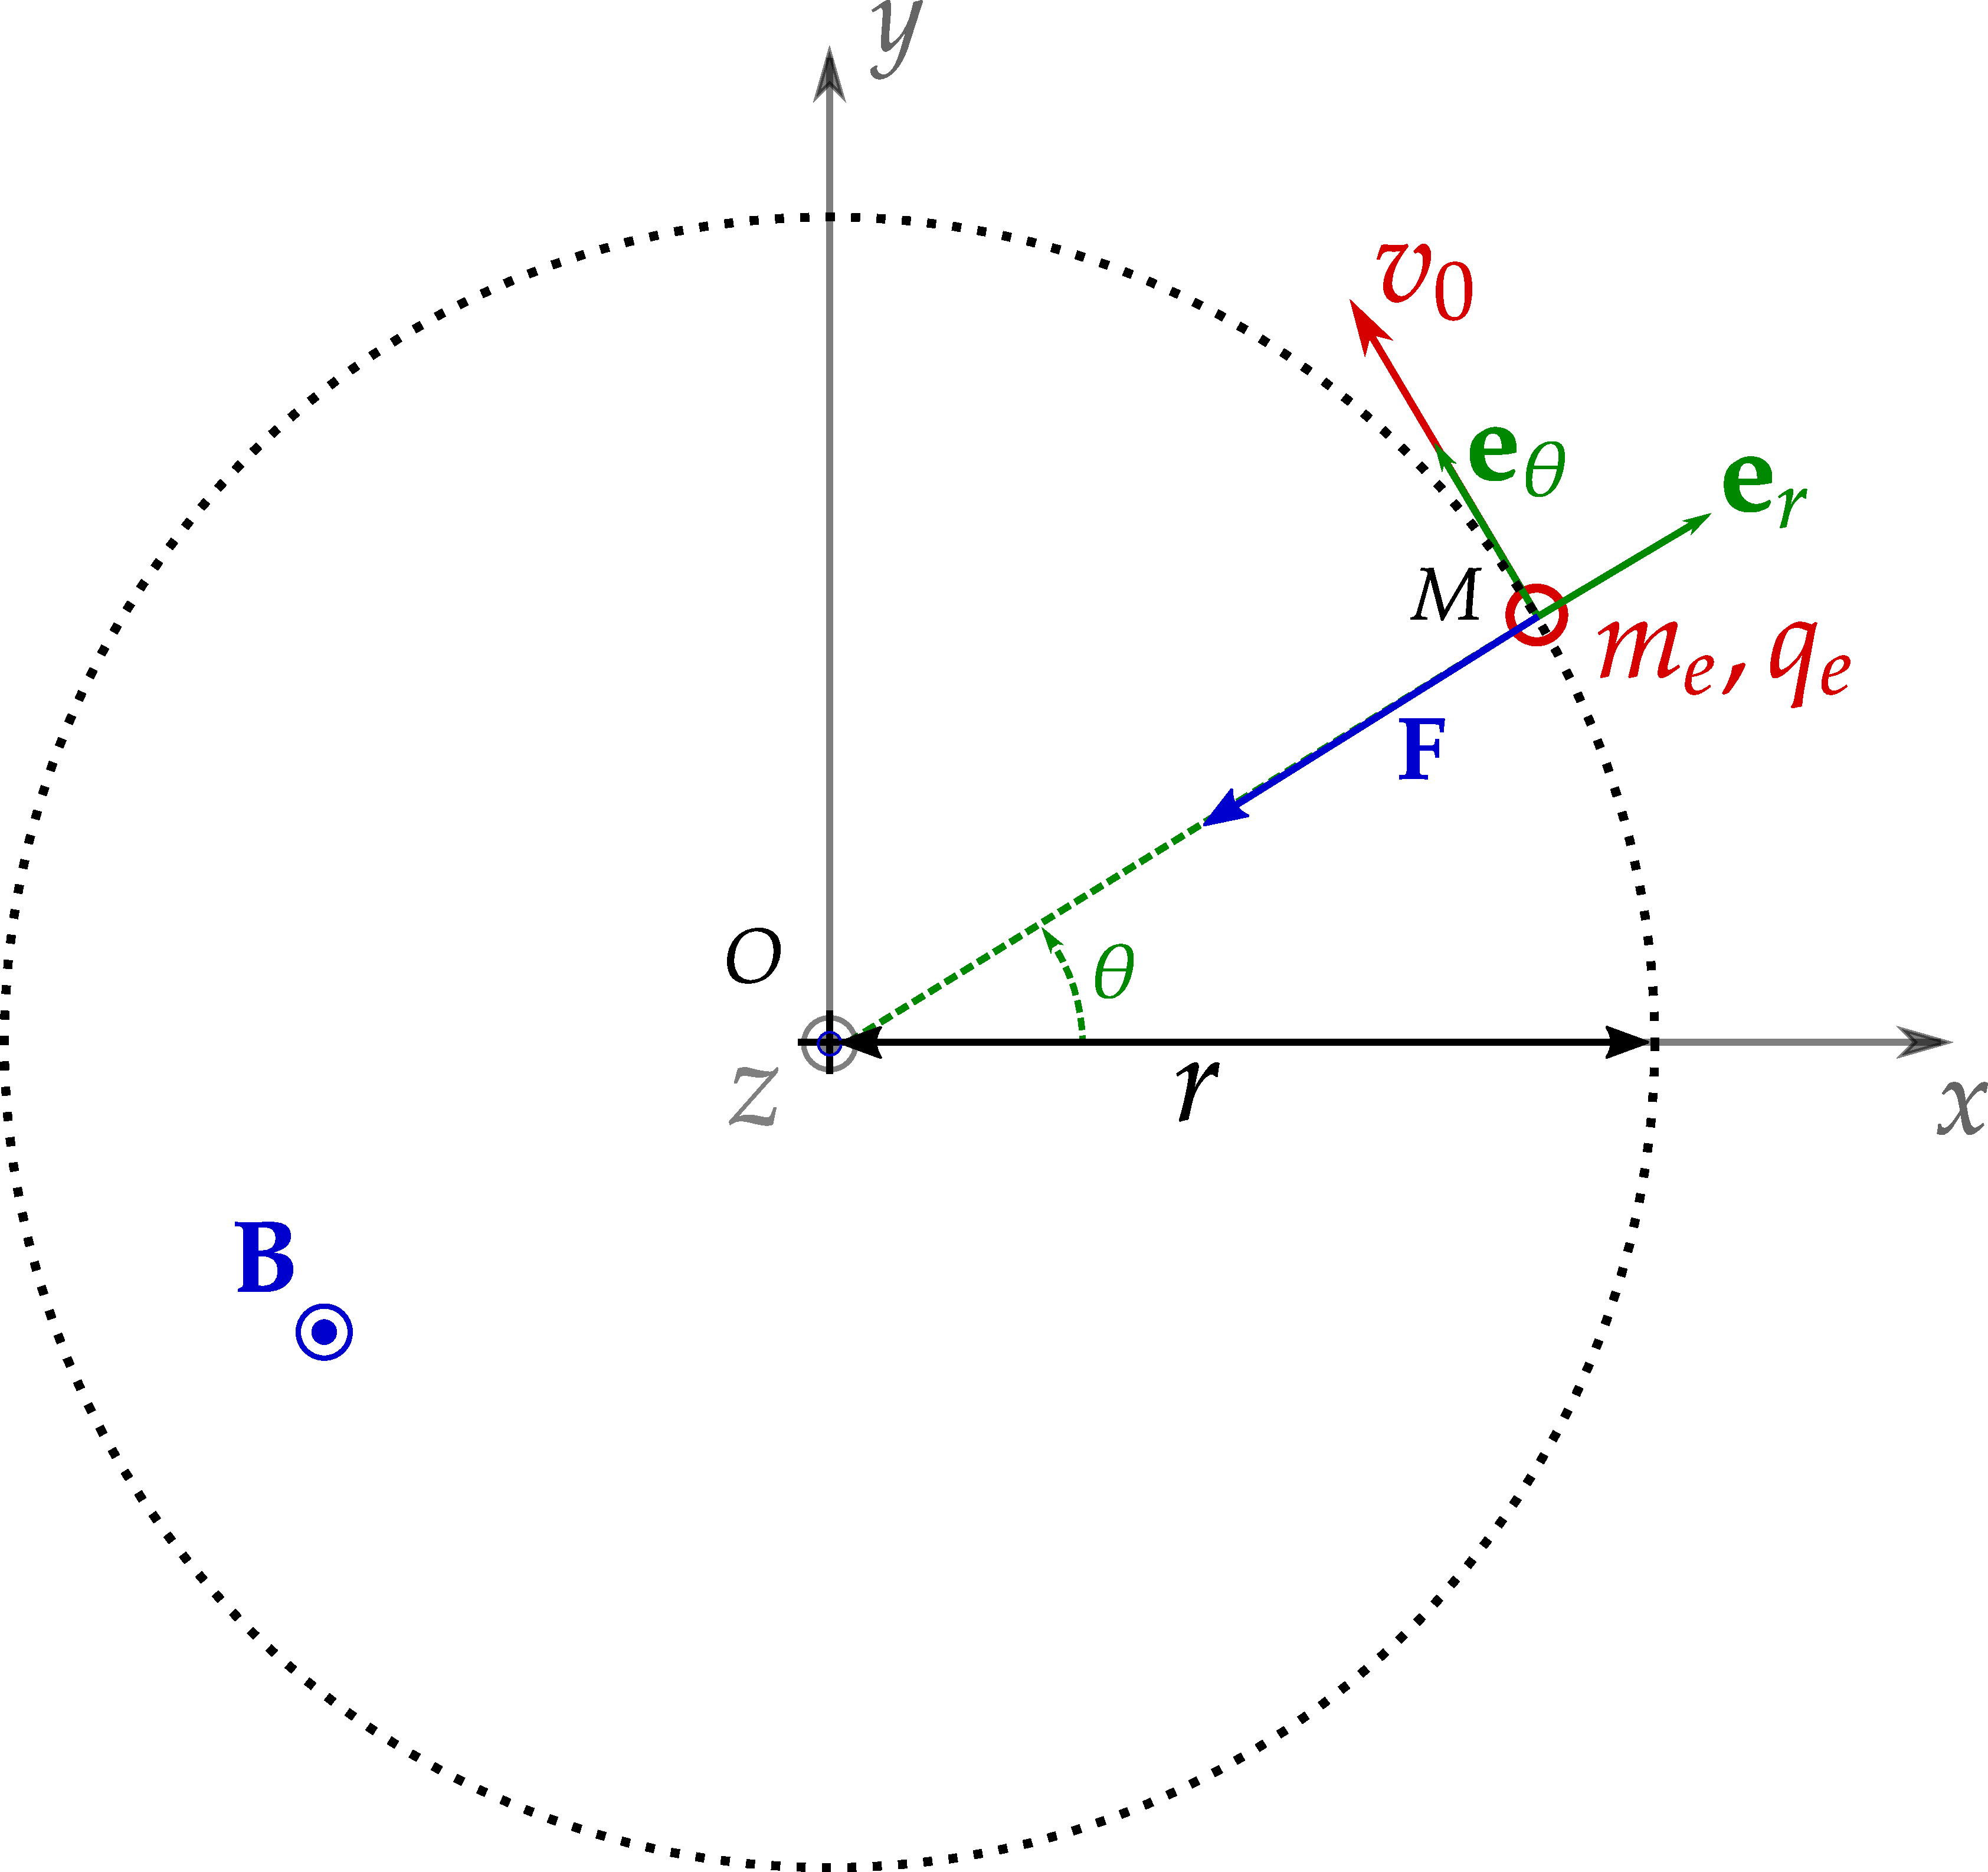
\includegraphics[scale=0.75]{cyclotron}
	\caption{Trajectoire d'un électron dans un champ magnétique uniforme.}%
	\label{fig:magneto_cyclotron}
\end{figure}

\section{La loi de Biot et Savart}
De la même manière que pour le champ électrostatique, nous
commençons par définir le champ magnétique généré par une charge ponctuelle. 
Soit une charge ponctuelle $q$ en un point $P$ de l'espace se déplaçant 
à la vitesse $\vecv$ dans le référentiel du laboratoire. Expérimentalement,
on observe que cette particule génère
en un point $M$ un champ magnétique $\vecb(M)$ tel que

\begin{equation*}
	\vecb(M) = \dfrac{\mu_0 q}{4 \pi} \vecv \wedge \dfrac{\mitbf{PM}}{||PM||^3},
\end{equation*}
où $\mu_0 = \unit{4 \pi \times 10^{-7}}{\tesla \usk \meter \usk \reciprocal 
\ampere}.$

\begin{figure}[h!]
	\centering
	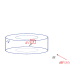
\includegraphics[]{biot_savart}
	\caption{Champ magnétique généré par un élément infinitésimal d'un conducteur
	de densité volumique de courant $\vecj$ en un point $M$ de l'espace.}%
	\label{fig:magneto_biot_savart}
\end{figure}

On considère un conducteur formant un volume $\mathcal{V}$ 
(voir Fig.~\ref{fig:magneto_biot_savart}) parcouru par des charges mobiles 
de densité volumique de charge $\rho$ se déplaçant à la vitesse $\vecv$. Un élément 
infinitésimal $\dV$ de ce circuit centré en $P$ génère en un point $M$ un champ magnétique

\begin{equation*}
	\mathrm{\textbf{d}}\mitbf{B}^P(M) = \dfrac{\mu_0 \rho(P) \dV}
	{4 \pi} \vecv(P) \wedge 
	          \dfrac{\mitbf{PM}}{||PM||^3},
\end{equation*}
où on reconnaît le vecteur densité de courant $\vecj(P) = \rho(P) \vecv(P)$. 
Le champ magnétique
$\vecb$ généré par l'ensemble du circuit en $M$ est alors obtenu en additionnant les 
contributions de chaque élément de ce dernier grâce au principe de superposition
\begin{equation*}
	\vecb(M) = \iiint_{P \in \mathcal{V}} \mathrm{\textbf{d}}\mitbf{B}^P(M)
		 = \iiint_{P \in \mathcal{V}} \dfrac{\mu_0}
		 {4 \pi} \vecj(P) \wedge 
	          \dfrac{\mitbf{PM}}{||PM||^3} \dV
\end{equation*}
On aboutit ainsi à la loi de Biot et Savart.

\begin{defn}[Loi de Biot et Savart]
	Le champ magnétostatique $\vecb(M)$ créé au point $M$ par une distribution
	volumique de courant $\vecj$ ($\ampere \usk \rpsquare \meter$) contenue
	dans un volume $\mathcal{V}$ est
	\begin{equation}
		\vecb(M) = \dfrac{\mu_0}{4 \pi} \iiint_{P \in \mathcal{V}} 
		\dfrac{\vecj(P) \wedge \mitbf{PM}}{||PM||^3} \dV,
	\end{equation}
	où $\mu_0 = \unit{4 \pi \times 10^{-7}}{\tesla \usk \meter \usk \reciprocal
	\ampere}$ est la perméabilité magnétique du vide.

\end{defn}

	Par un raisonnement similaire, on montre que pour une distribution 
	surfacique de courant $\vecj_s$ confinée sur une 
	surface $\mathcal{S}$, cette expression devient
	\begin{equation}
		\vecb(M) = \dfrac{\mu_0}{4 \pi} \iint_{P \in \mathcal{S}} 
		\dfrac{\vecj_s(P) \wedge \mitbf{PM}}{||PM||^3} \mathrm{d}S.
	\end{equation}

	Pour un circuit filiforme $\mathcal{C}$ parcouru par un courant $I$, 
	cette expression devient
	\begin{equation}
		\vecb(M) = \dfrac{\mu_0}{4 \pi} \int_{P \in \mathcal{C}} 
	\dfrac{I \dl \wedge \mitbf{PM}}{||PM||^3}.
	\end{equation}

\begin{exemple}
	On cherche à déterminer le champ magnétique généré par un fil infini $\mathcal{C}$
	parcouru
	par un courant d'intensité $I$ en un point $M$ 
	(voir Fig.~\ref{fig:magneto_spire}). On se place dans un repère cylindrique
	$(0, \er, \etheta, \ez)$. Les points $M$ et $P$ ont pour coordonnées 
	respectives $(r, \theta, 0)$ et $(0, 0, z_P)$.

	Le champ magnétique $\mathrm{\textbf{d}}\vecb^P(M)$ généré par un élément
	$\dl_P$ du fil centré en $P$ s'écrit
	\begin{equation*}
	\mathrm{\textbf{d}}\vecb^P(M) = \dfrac{\mu_0}{4 \pi} 
	              \dfrac{I \dl_P \wedge \mitbf{PM}}{||PM||^3},
	\end{equation*}
	où $\mitbf{PM} = \mitbf{PO} + \mitbf{OM} = - z_P\ez + r\er$. Dans un repère
	cylindrique, un élément infinitésimal $\dl_P$ du fil s'écrit
	$\dl_P = \dz_P \ez$. On a alors
	\begin{equation*}
		\dfrac{\dl_P \wedge \mitbf{PM}}{||PM||^3} = 
		\dfrac{r\dz_P}{||PM||^3}\etheta. 	
	\end{equation*}
	En remarquant que $||PM|| = r/\cos\alpha$, l'expression précédente devient alors
	\begin{equation*}
		\dfrac{r\dz_P}{||PM||^3}\etheta = \dfrac{\cos^3\alpha \dz_P}
		{r^2} \etheta
	\end{equation*}
	De même, on remarque que $z_p = r \tan\alpha$.
	Par différentiation, on obtient donc
	\begin{equation*}
		\dz_P = \mathrm{d}\left[r\tan\alpha\right] = 
		\dfrac{r \mathrm{d}\alpha}{\cos^2\alpha}.
	\end{equation*}
	Finalement,
	\begin{equation*}
		\mathrm{\textbf{d}}\vecb^P(M) = \dfrac{\mu_0 I \cos\alpha}
		{4 \pi r} \mathrm{d}\alpha \etheta.
	\end{equation*}
	Le champ $\vecb(M)$ généré au point $M$ par le fil s'obtient alors
	en utilisant le principe de superposition, ce qui revient à intégrer les champs 
	magnétiques infinitésimaux sur l'ensemble du fil. Pour parcourir l'ensemble du
	fil, $\alpha$ doit varier entre $-\pi/2$ et $\pi/2$. On a alors
	\begin{equation*}
		\boxed{\vecb(M) = \dfrac{\mu_0 I}{4\pi r}
			\times \displaystyle{\int_{-\pi/2}^{\pi/2} 
			\cos\alpha\mathrm{d}\alpha \etheta} =
	\dfrac{\mu_0 I}{2\pi r}\etheta.}
	\end{equation*}
	On obtient un champ magnétique porté par $\etheta$ et donc la norme ne dépend
	que de $r$. Les lignes de ce champ sont des cercles concentriques centrés
	sur le fil. $\vecb$ "tourne" autour du fil.
\end{exemple}
\begin{figure}[h!]
	\centering
	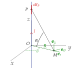
\includegraphics[scale=0.7]{fil}
	\caption{Champ magnétique créé en un point $M$ par un fil parcouru par
	un courant d'intensité $I$.}%
	\label{fig:magneto_spire}
\end{figure}

\begin{defn}[Calcul du champ magnétique par la loi de Biot et Savart]
	Comme nous l'avons vu dans l'exemple précédent, la loi de Biot et Savart
	peut s'avérer utile lorsqu'il s'agit de calculer le champ magnétique 
	$\vecb$ généré par une distribution de courant. Voici en résumé la démarche à suivre
	\begin{enumerate}
		\item Réaliser un schéma du système et choisir un repère adapaté.
		\item Exprimer le petit volume $\dV$, de surface $\mathrm{d}S$
		  ou de longueur $\dl$ dans ce système de coordonnées.
	  \item En multipliant cet élément par le courant ($\vecj$, $\vecj_s$ ou
	    $I$), on obtient le petit élément de courant associé.
	  \item Exprimer le vecteur $\mitbf{PM}$ dans le système de coordonnées
	    choisi.
    	\item En multipliant par $\dfrac{\mu_0}{4 \pi}$ et en faisant le produit 
	  vectoriel par $\dfrac{\mitbf{PM}}{||PM||^3}$, on fabrique le champ
	  élémentaire $\mathrm{\textbf{d}}\vecb^P(M)$ généré en $M$.
	\item Pour calculer $\vecb(M)$, il suffit alors d'intégrer sur la distribution
	  de courant.
	\end{enumerate}
\end{defn}
\section{Équation de la magnétostatique}
On considère un fil parcouru par un courant $I$ dans un
repère cylindrique $(O, \er, \etheta, \ez)$ (voir Fig.~\ref{fig:magneto_spire}). 
Comme vu ci-dessus, le champ
magnétique créé par ce fil en un point $M$ situé à une distance $r$ du fil
est donné par
\begin{equation*}
	\vecb(M) = \dfrac{\mu_0 I}{2 \pi r}\etheta.
\end{equation*}
Comme pour le champ électrostatique, nous allons nous servir de cet exemple simple 
pour retrouver certaines propriétés du champ magnétostatique.

\subsection{Le théorème d'Ampère}
Le théorème d'Ampère est l'équivalent pour le champ magnétostatique $\vecb$
du théorème de Gauss. Il va nous permettre de calculer facilement le champ
magnétostatique généré par une distribution de courants simple.

Les lignes du champ $\vecb$ créé par le fil sont des cercles dont l'axe est le
fil. Nous cherchons donc dans un premier temps à calculer la circulation de $\vecb$ 
sur la ligne de champ $\mathcal{C}$ de rayon $r$ passant par $M$. 
On a bien pris soin au préalable
d'orienter cette dernière. Dans un repère cylindrique, un petit élément $\dl$ de ce 
contour fermé s'écrit $\dl = r \dtheta \etheta$. La circulation de $\vecb$ sur
ce contour s'écrit donc
\begin{equation*}
	\boxed{\displaystyle{\oint_\mathcal{C} \vecb \cdot \dl = 
		\oint_0^{2 \pi} \dfrac{\mu_0 I}{2 \pi r} r\dtheta
	= \mu_0 I.}}
\end{equation*}
On constate que la circulation du champ $\vecb$ le long du circuit $\mathcal{C}$
ne dépend que du courant $I$ que ce dernier enlace. Cette propriété que nous venons
de montrer pour un fil est en fait une propriété générale du champ magnétostatique.

\begin{defn}[Théorème d'Ampère]
	La circulation du champ magnétostatique $\vecb$ le long d'un circuit fermé
	$\mathcal{C}$ est égale au courant \textbf{algébrique} $I_\mathrm{int}$ 
	enlacé par ce dernier multiplié
	par $\mu_0$
	\begin{equation}
		\oint_\mathcal{C} \vecb \cdot \dl = \mu_0 I_\mathrm{int}.
	\end{equation}
	Le contour sur lequel est réalisée l'intégrale est appelé contour d'Ampère.
	Le courant enlacé $I_\mathrm{int}$ est le courant qui traverse une surface 
	orientée
	qui s'appuie sur le contour d'Ampère. L'orientation de la surface 
	se déduit de celle du contour
	grâce à la règle de la main droite ou du tire-bouchon.
\end{defn}

\begin{exemple}
	\begin{minipage}{0.6\linewidth}
	Soit deux fils électriques parcourus par des courants $I_1$ et $I_2$.
	Avec les orientations choisies, le théorème d'Ampère appliqué au 
	contour $\mathcal{C}$ s'écrit
	\begin{equation*}
		\oint_\mathcal{C} \vecb \cdot \dl = \mu_0(I_1 - I_2).
	\end{equation*}
	\end{minipage}
	\hfill
	\begin{minipage}{0.35\linewidth}
		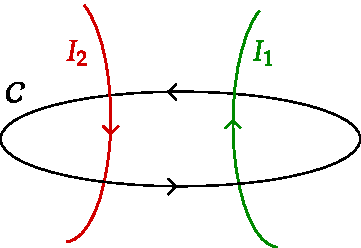
\includegraphics[width=0.8\linewidth]{ampere_ex}
	\end{minipage}

\end{exemple}

Le théorème d'Ampère peut-être traduit sous une forme locale:
appelée \textbf{équation de Maxwell-Ampère}, qui relie alors le champ magnétostatique
au vecteur densité de courant.

\begin{defn}[Équation de Maxwell-Ampère]
	L'équation de Maxwell-Ampère relie le champ magnétostatique $\vecb$
	au vecteur densité de courant $\vecj$
	\begin{equation}
		\rot \vecb = \mu_0 \vecj.
		\label{eq:magneto_ma}
	\end{equation}
	Cette équation est une relation $\textbf{locale}$, elle permet de relier 
	les dérivées spatiales du champ $\vecb$ en un point de l'espace au vecteur
	$\vecj$ en ce même point.
\end{defn}

\subsection{Flux du champ magnétostatique $\vecb$}
On cherche maintenant à calculer la divergence du champ $\vecb$. En coordonnées 
cylindriques, cela donne
\begin{equation*}
	\div \vecb = \dfrac{1}{r}\left(\dd{r B_r}{r} + \dd{B_\theta}{\theta} \right)
	+ \dd{B_z}{z},
\end{equation*}
où $B_r$, $B_\theta$ et $B_z$ sont les composantes de $\vecb$. 
Dans le cas du fil infini, $B_\theta$ est la seule composante non nulle de $\vecb$ 
et elle ne dépend pas
de $\theta$. On a donc
\begin{equation*}
	\div \vecb = 0.
\end{equation*}
Ce résultat se généralise à un champ magnétostatique $\vecb$ quelconque sous
la forme de l'équation de Maxwell-Thomson.

\begin{defn}[Équation de Maxwell-Thomson]
	Un champ magnétique $\vecb$ vérifie toujours
	\begin{equation*}
		\div \vecb = 0.
	\end{equation*}
	Cette relation locale est vérifiée en tout point de l'espace.
\end{defn}

\begin{rem}
La divergence de $\vecb$ étant nulle, l'analyse vectorielle affirme
qu'il est possible dans ce cas de définir un champ vectoriel $\veca$,
défini à un gradient près, tel que $\rot \veca = \vecb$,
appelé le potentiel vecteur.
\end{rem}

Comme l'équation de Maxwell-Ampère, cette équation peut se mettre sous une forme
intégrale, en exprimant le flux du champ magnétique à travers une surface fermée
$\mathcal{S}$.

\begin{defn}[Flux du champ magnétostatique]
	Le flux du champ magnétique $\vecb$ à travers une surface fermée 
	$\mathcal{S}$ est nul
	\begin{equation*}
		\oiint_\mathcal{S} \vecb \cdot \ds = 0.
	\end{equation*}
	On dit que le champ $\vecb$ est à flux conservatif.
\end{defn}

	\begin{minipage}{0.6\linewidth}
	On peut appliquer ce résultat à une surface $\mathcal{S}$ particulière
	constituée d'une portion de tube de champ de section d'entrée $\mathcal{S}_e$,
	de section de sortie $\mathcal{S}_s$ et de section latérale $
	\mathcal{S}_l$. 	
	\end{minipage}
	\hfill
	\begin{minipage}{0.3\linewidth}
	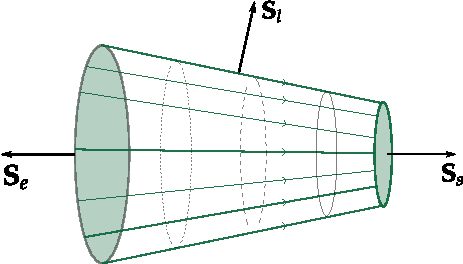
\includegraphics[scale=0.7]{tube}
	\end{minipage}
	\vspace{0.5cm}

\begin{defn}[Tube de champ]
	L'ensemble des lignes de champ s'appuyant sur un contour fermé forme un 
	tube de champ.
\end{defn}
	
	D'après le théorème d'Ampère la flux de $\vecb$ à
	travers cette surface est nul.
	Par définition du tube de champ, l'intégrale sur la surface 
	latérale est nulle. Il reste donc 
	\begin{equation*}
		\iint_\mathcal{S_e} \vecb \cdot \ds_e =
		- \iint_\mathcal{S_s} \vecb \cdot \ds_s 
		\iff
		\displaystyle{\left\lvert\iint_\mathcal{S_e} \vecb \cdot \ds_e\right\rvert =
		\left\lvert\iint_\mathcal{S_s} \vecb \cdot \ds_s\right\rvert}.
	\end{equation*}
	Le flux entrant dans la surface est égal au flux sortant de cette dernière.
	De plus, la surface de sortie étant de taille plus importante que 
	la surface d'entrée, on en conclut que le champ est plus intense
	à l'entrée du tube qu'à la sortie. Le champ $\vecb$ étant à flux
	conservatif, un resserrement des lignes de champs traduit une augmentation
	de l'intensité de ce dernier.

\begin{defn}[Flux conservatif et lignes de champ]
	Le champ magnétique étant à flux conservatif, ses lignes de champs
	se resserrent dans les zones de forte intensité. Inversement, ces dernières
	s'éloignent lorsqu'il devient plus faible
\end{defn}

\section{Étude des lignes de champ de \vecb}
Nous nous intéressons dans cette partie aux propriétés spatiales du champ $\vecb$.
Nous allons voir comment les \textbf{lignes de champ} nous renseignent sur sa répartition 
dans l'espace.

Nous nous intéressons au champ magnétique produit par un solénoïde 
(voir Fig.~\ref{fig:magneto_solenoide}).
Les lignes de champ nous permettent de retrouver quelques propriétés du champ 
magnétostatique énoncées précédemment.

\begin{figure}[htpb]
	\centering
	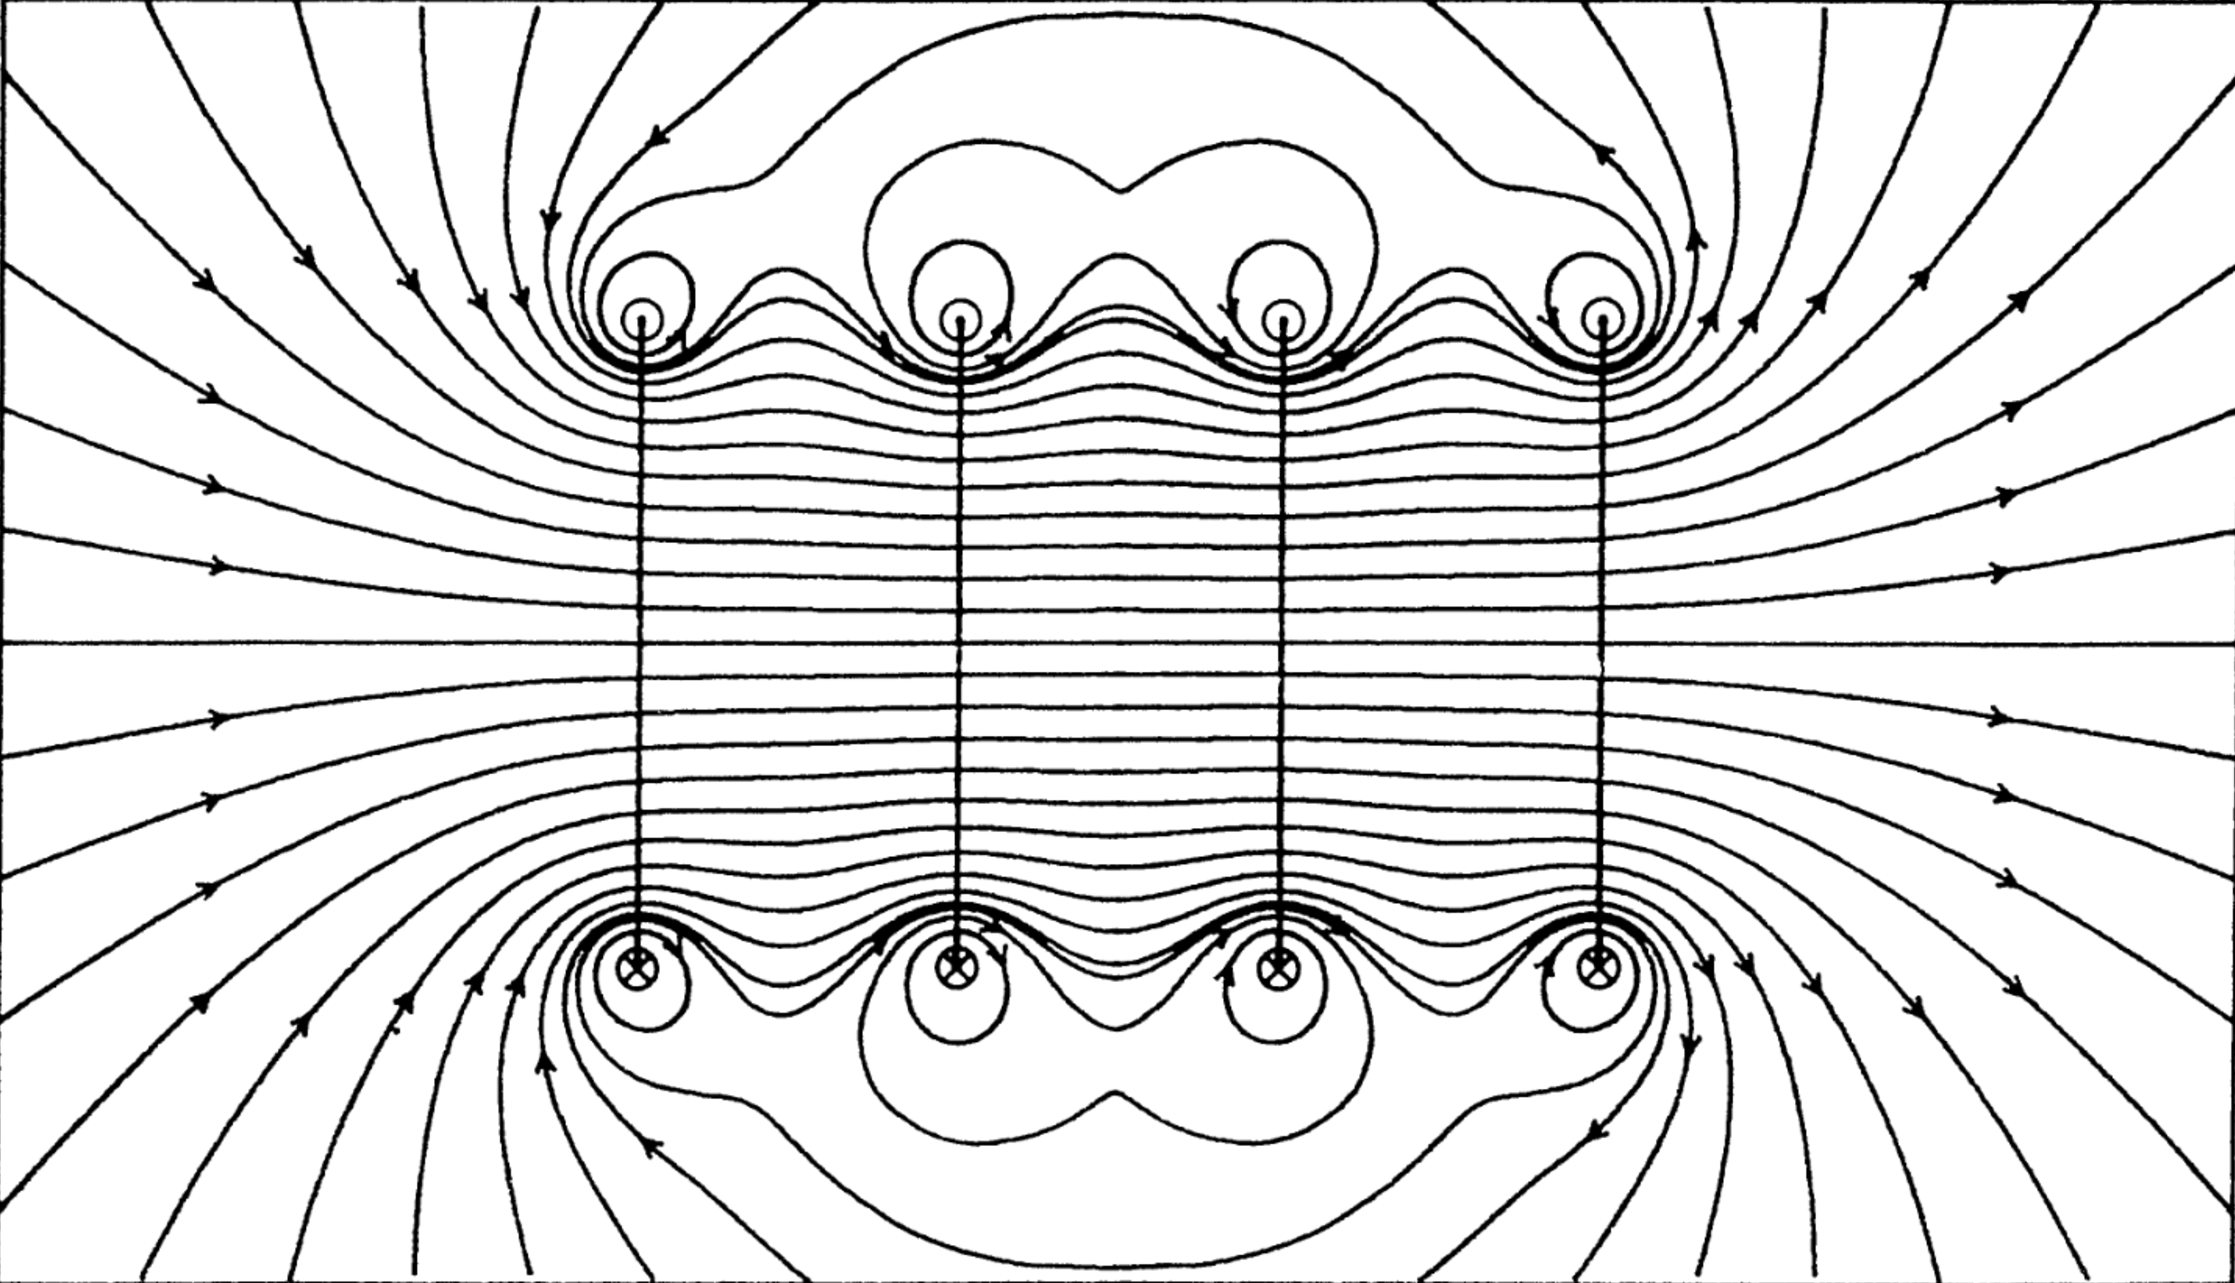
\includegraphics[width=0.7\linewidth]{solenoide}
	\caption{Lignes du champ magnétique généré par un solénoïde constitué de
		4 bobines parcourues dans le même sens par la même intensité.
		Cette figure est extraite de \cite{Gie1985}}%
	\label{fig:magneto_solenoide}
\end{figure}

\begin{enumerate}
	\item On remarque tout d'abord que les lignes de champ 
	  sont des contours fermés qui entourent les fils parcourus par un courant.
	  Cette première observation est une conséquence directe de l'équation
	  de Maxwell-Ampère. L'orientation de ces lignes de champ s'obtient
	  d'ailleurs en considérant le sens du courant dans les fils et en utilisant
	  la règle de la main droite.
      \item La divergence nulle de $\vecb$ est aussi visible sur cette carte de 
	champ. En effet, on constate que les lignes de champ ne convergent/divergent
	pas en un point de l'espace, contrairement au champ électrostatique.
      \item Dans le cas du champ magnétique, le resserrement des lignes de champ
	traduit une augmentation de la norme de ce dernier. On conclut que le champ
	est plus intense à l'intérieur du solénoïde qu'à l'extérieur. De plus, les
	lignes de champ étant parallèles à l'intérieur du solénoïde, on conclut que
	le champ est uniforme.
      \item Grâce aux lignes de champ, on retrouve rapidement les plans de 
	  symétrie et d'antisymétrie du champ magnétique. Le plan médiateur 
	  du solénoïde est par exemple un plan de symétrie du champ magnétique. 
          L'analyse de ces symétries sera utile pour calculer le champ
          magnétique résultant d'une distribution de courant.
\end{enumerate}

\section{Calcul du champ magnétostatique}
\label{sec:calcul_e}
Nous allons voir dans cette partie comment nous pouvons utiliser le théorème d'Ampère
pour calculer le champ magnétostatique $\vecb$ créé 
par une distribution de courants simple. Nous nous intéressons ici à une bobine
torique constituée d'un fil régulièrement bobiné autour d'un tore de section
carré (voir Fig.~\ref{fig:magneto_tore}). Cette bobine est caractérisée par le nombre $N$
total de spires bobinés, son rayon intérieur $R$ 
et sa hauteur $h$. La bobine est parcourue par un courant $I$.

On cherche à déterminer 
l'expression du champ électrique $\vecb$ en un point $M$ de l'espace. Pour ce faire, 
il suffit de suivre le mode d'emploi suivant
\begin{enumerate}
	\item Faire un schéma du système ! C'est absolument indispensable
	  (voir Fig.~\ref{fig:magneto_tore})
	\item Choisir un repère adapté au problème
	\item Étudier les invariances de cette distribution
	\item Étudier les symétries de la distribution de courants à l'origine 
	  du champ magnétostatique
	\item Choisir un contour d'Ampère et appliquer le théorème d'Ampère.
\end{enumerate}

Au vu de la géométrie du système, nous choisissons ici d'utiliser 
un repère cylindrique $(O, \er, \etheta, \ez)$.
Le point $M$ est donc repéré par ses coordonnées $(r, \theta, z)$. Le champ
magnétostatique en $M$ s'écrit de manière générale

\begin{equation}
	\vecb(M) = B_r(M)\er + B_\theta(M)\etheta + B_\varphi(M)\ephi.
	\label{eq:tore}
\end{equation}
Le champ magnétostatique est un vecteur à trois composantes et chaque composante
dépend des coordonnées de $M$. Pour simplifier cette expression, il est intéressant
de considérer les invariances et symétries de la distribution de courant qui génère
le champ $\vecb$.

\begin{figure}
	\centering
	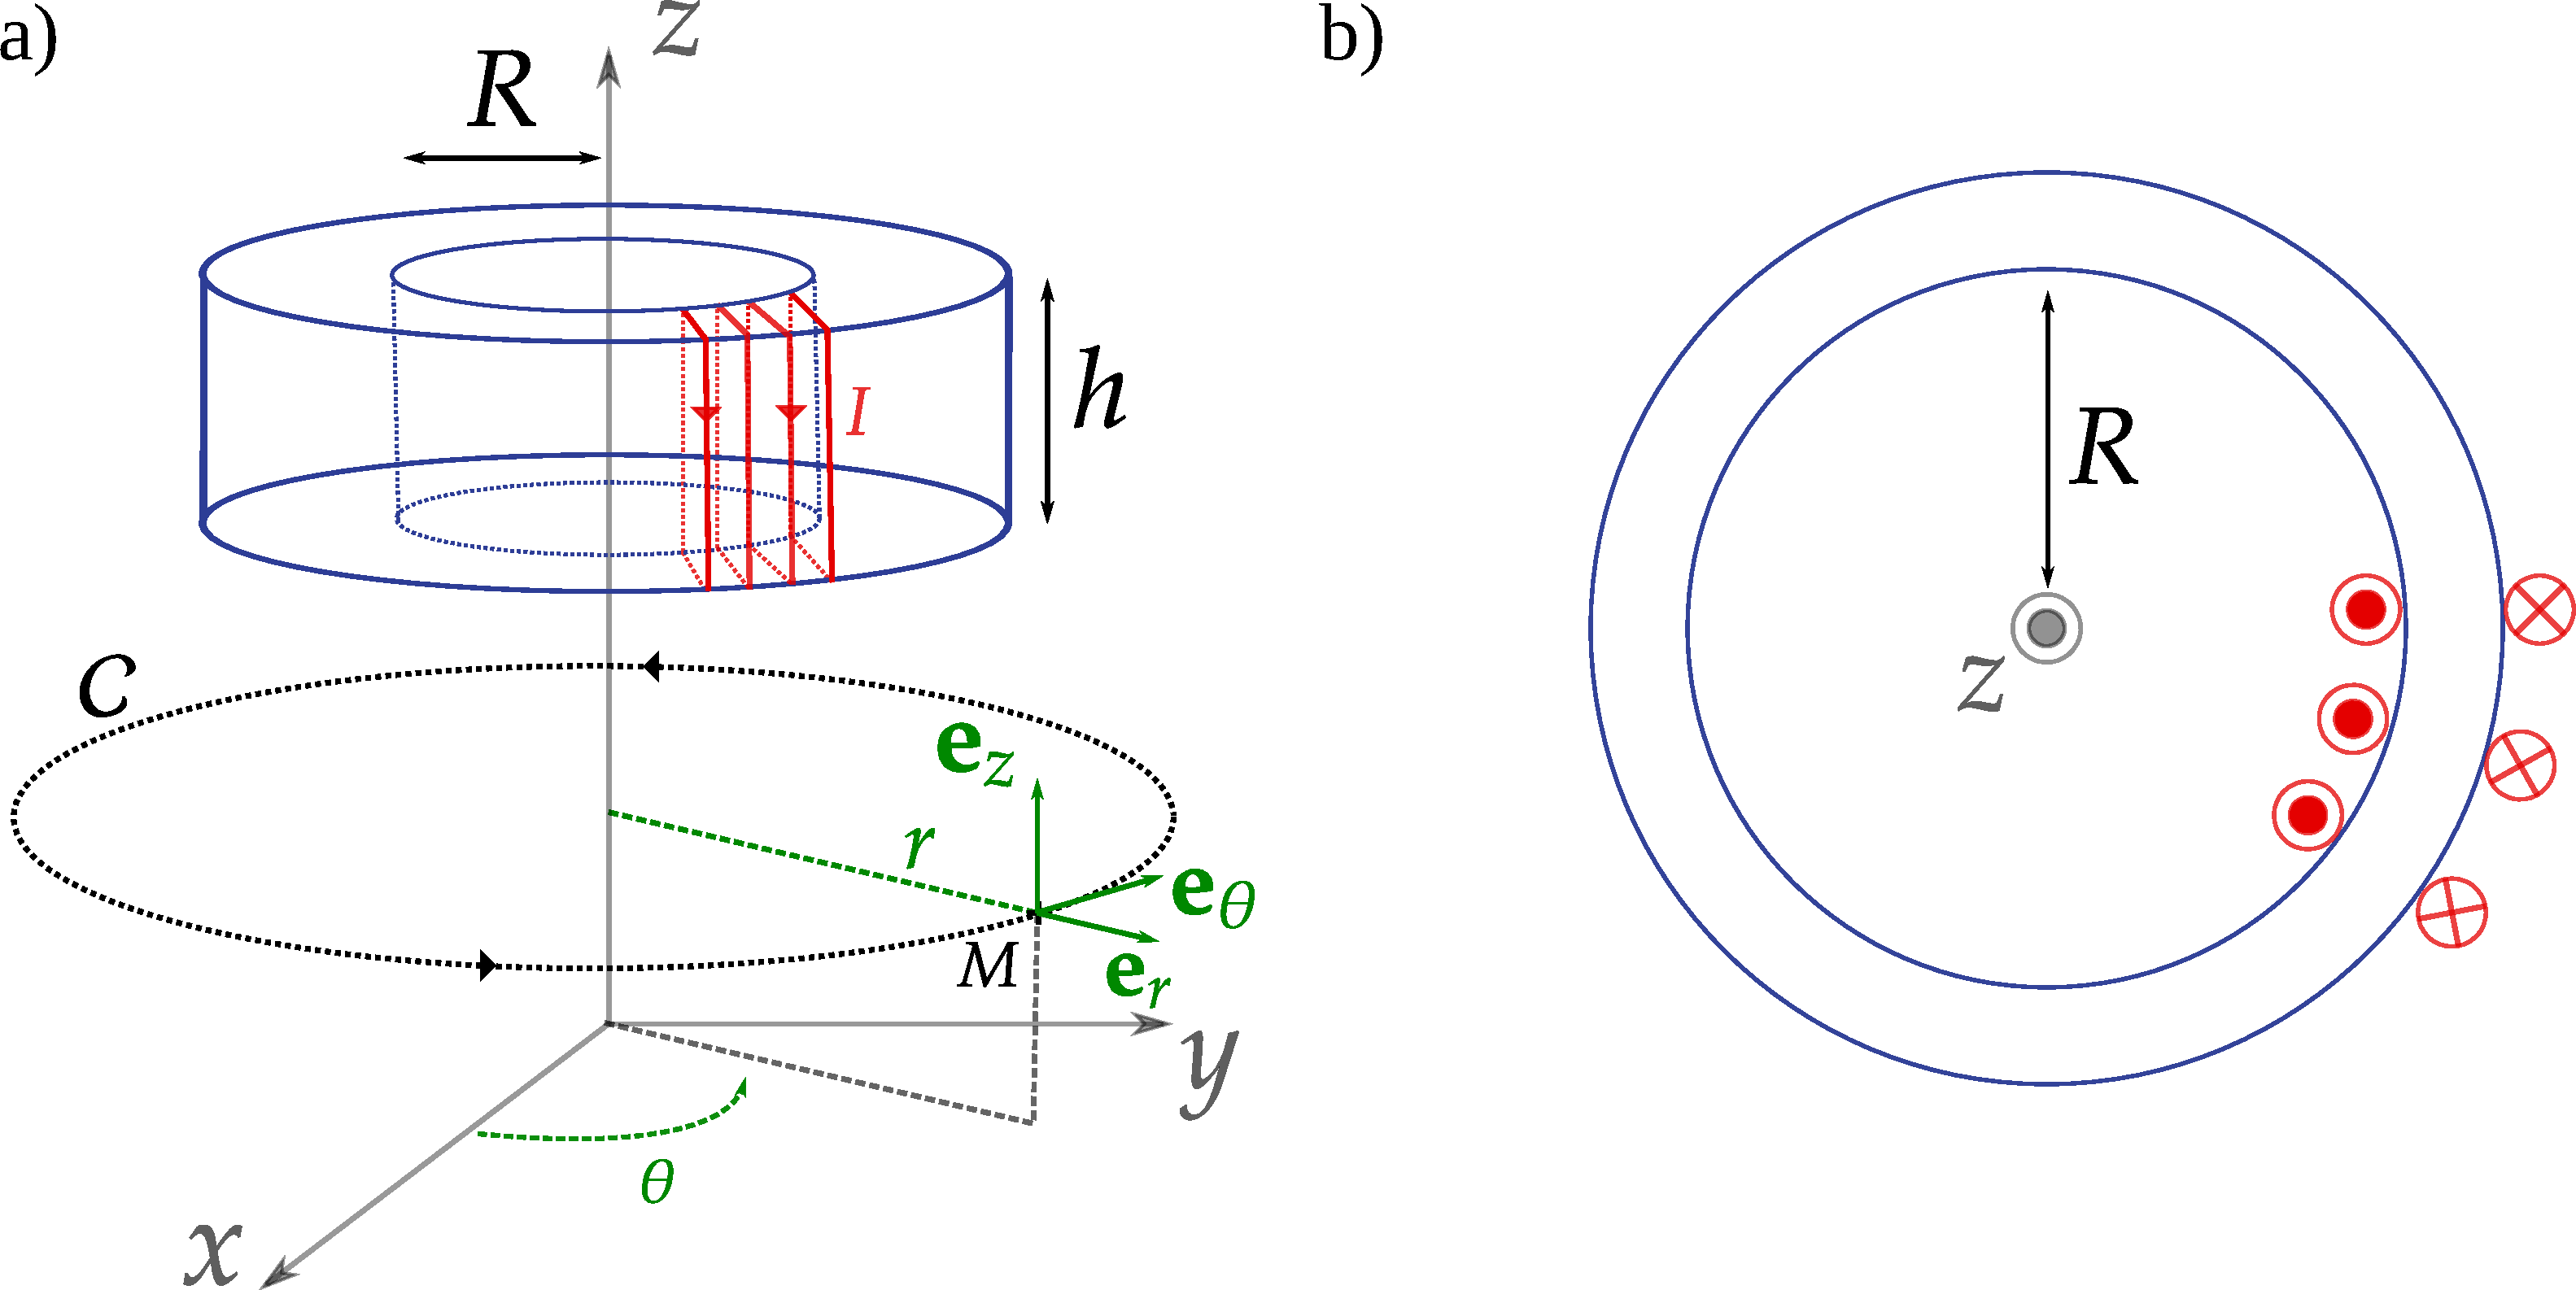
\includegraphics[scale=1]{tore}
	\caption{Bobine torique à gauche et coupe perpendiculaire à $(Oz)$
	de cette bobine à droite.}%
	\label{fig:magneto_tore}
\end{figure}

\subsection{Invariance de la distribution de courants}
On cherche ici à savoir si la distribution de courant est modifiée sous l'effet
d'une translation ou d'une rotation de l'espace. En d'autres termes, on regarde
de quelles variables elle dépend. Étant donné que les spires sont uniformément
répartie sur le tore, on observe que

\begin{itemize}
	\item  si je tourne le tore d'un angle $\Delta \theta$ dans la
	  direction $\etheta$, le problème
	  ne change pas. La distribution de courant est donc invariante 
	  par rotation selon l'angle $\theta$. $\vecb$ \textbf{ne dépend pas de
	  $\mitbf{\theta}$}.
\end{itemize}

Finalement, l'expression~\ref{eq:tore} du champ magnétique se simplifie donc en 

\begin{equation*}
	\boxed{\vecb(M) = B_r(r,z)\er + B_\theta(r,z)\etheta + B_z(r,z)\ez.}
\end{equation*}
\subsection{Symétries de la distribution de courants}

Si on applique ce principe au champ magnétique créé par une distribution 
de courants, cela revient à dire que les symétries de la distributions de 
courants doivent se retrouver dans les symétries du champ magnétique. On en 
déduit les règles suivantes

\begin{defn}[Symétries de $\vecb$ et de la distribution de courant]
\begin{itemize}
  \item si $(\Pi)$ est un plan d'antisymétrie de la distribution de courant et que 
    $M$ appartient à $(\Pi)$, alors obligatoirement $\vecb(M)$ doit 
    appartenir à $(\Pi)$,
  \item si $(\Pi)$ est un plan de symétrie de la distribution de courant 
    et que $M$ appartient à $(\Pi)$, alors obligatoirement $\vecb(M)$ doit 
    être orthogonal à $(\Pi)$.
\end{itemize}
\end{defn}

\begin{rem}
	Le champ magnétostatique $\vecb$ appartient aux plans d'\textbf{antisymétrie}
	de la distribution de courant et non aux plans de symétrie comme
	c'est le cas pour le champ électrostatique. Le vecteur $\vecb$ est 
	qualifié de vecteur axial.
\end{rem}

Pour appliquer ces règles à notre exemple, on détermine les plans de symétrie 
et d'antisymétrie de la distribution de courants auquels 
le point $M$ appartient

\begin{itemize}
	\item le plan $(M, \er, \ez)$ est un plan de symétrie de la distribution
	  de courant. $\vecb(M)$ \textbf{doit être orthogonal à ce plan}.
\end{itemize}

$\vecb(M)$ doit être orthogonal au plan $(M, \er, \ez)$, 
il doit donc être colinéaire à $\etheta$

\begin{framed}
\begin{equation*}
	\vecb(M) = B_\theta(r, z) \etheta.
\end{equation*}
\end{framed}

Nous n'avons imposé aucune condition sur la position de $M$, cette relation est
donc vraie pour tout point $M$ de l'espace. Maintenant que l'expression du 
champ magnétique a été simplifiée au maximum, on cherche à appliquer le théorème
d'Ampère.

\subsection{Application du théorème d'Ampère}
La distribution de courant présente une symétrie de révolution. On choisit comme contour 
d'Ampère un cercle $\mathcal{C}$ de rayon $r$, de centre $O$ et orienté
dans le sens de $\etheta$ qui passe par $M$ 
(voir Fig~\ref{fig:magneto_tore}) et on applique le théorème d'Ampère à ce dernier

\begin{equation*}
	\oint_\mathcal{S} \vecb(M) \cdot \dl = \mu_0 I_\mathrm{int},
	\label{eq:cavite_gauss}
\end{equation*}
où $I_\mathrm{int}$ est la courant enlacé par $\mathcal{C}$. On commence
par déterminer l'expression du membre de gauche. Dans un repère cylindrique,

\begin{equation*}
	\dl = r \dtheta \etheta.
\end{equation*}
On obtient alors
\begin{equation*}
	\oint_\mathcal{C} \vecb(M) \cdot \dl = 
	\oint_\mathcal{C} B(r,z) \etheta \cdot r \dtheta \etheta
	= B(r, z) r \int_0^{2 \pi} \dtheta
	= 2 \pi r B(r,z).
\end{equation*}
On s'intéresse maintenant au terme de droite de l'équation.
Deux cas de figure se présentent:
\begin{itemize}
	\item $M$ est situé dans le tore: le courant enlancé par $\mathcal{C}$ est alors
	  $I_\mathrm{int} = NI$.
       \item $M$ est situé à l'extérieur du tore: le courant enlacé par 
	       $\mathcal{C}$ est donc nul. Soit parce que le contour n'enlace 
	       aucun courant, soit parce qu'il enlace autant de courants positifs
	       que de courants négatifs.
\end{itemize}
Finalement,
\begin{framed}
\begin{itemize}
	\item si $M$ se trouve à l'intérieur du tore, 
	  $\vecb(M) = \dfrac{\mu_0 N I}{2 \pi r} \etheta$.
	\vspace{1em}
\item si $M$ est en dehors du tore, $\vecb(M) = \mitbf{0}$. 
\end{itemize}
\end{framed}
%\nocite{*}
%\putbib[magnetostatique]

%\newpage

%\chapter{Magnétostatique}
\label{chap:magnetostatique}
\section*{Objectifs}%
\label{sec:objectifs}
\begin{itemize}
	\item Connaître les équations qui contrôlent l'évolution spatiale 
	  du champ magnétostatique $\vecb$.
	\item Faire le lien entre ces équations et une carte de champ 
	  magnétique.
	\item Savoir calculer le champ magnétostatique résultant d'une 
	  distribution simple de courants.
\end{itemize}
\newpage
\section*{Introduction}
La magnétostatique étudie les champs magnétiques créés par des courants permanents.
Le plus souvent, on cherche alors à déterminer le champ magnétostatique $\vecb$
qui résulte d'une distribution de courant $\vecj$ connue. Nous nous intéressons
dans ce chapitre au champ magnétique créé par des courants circulants 
dans des conducteurs. Les milieux aimantés seront abordés plus loin dans le cours.

\section{La force de Lorentz}%
L'interaction entre deux particules immobiles a permis de définir la force de 
Coulomb dans le chapitre~\ref{chap:electrostatique}. Cette interaction 
électrostatique ne suffit plus lorsqu'il s'agit de décrire la dynamique de 
charges en mouvement. En 1895, le physicien néerlandais Hendrick Antoon Lorentz
propose alors l'ajout d'un second terme à la force coulombienne qui fait apparaître
la champ magnétostatique $\vecb$. 

\begin{defn}[Champ magnétostatique]
	Au même titre que le champ électrostatique, le champ magnétique $\vecb$
	est un champ vectoriel. Il est généré par une distribution de courant ou 
	par un aimant. Il s'exprime en tesla, noté $\tesla$ ($\kilogram \usk
	\rpsquare \second \reciprocal \ampere$ en SI). On rappelle quelques ordres de
	grandeur du champ magnétique
	
	\begin{center}
	\begin{tabular}{l|l}
		\textbf{Dispositif} 	& $\vecb (\tesla)$ \\ \hline
		Champ magnétique terrestre à la surface & $47 \times 10^{-6}$ \\
		Champ créé à $\unit{1}{\centi \meter}$ d'un fil parcouru par 
		un courant de $\unit{10}{\ampere}$
								 & $2 \times 10^{-5}$ \\
		Champ créé à $\unit{1}{\milli \meter}$ d'un aimant permanent& $0.1 - 1$ \\
		Électroaimant & $10 - 100$ \\
		Étoile à neutrons en surface & $10^{11}$\\
	\end{tabular}
	\end{center}
Le champ magnétique vérifie lui aussi le principe de superposition.
\end{defn}

\begin{defn}[Force de Lorentz]
Une particule de charge $q$ se déplaçant à la vitesse $\vecv$ dans un champ magnétique
$\vecb$, subit une force appelée force de Lorentz
\begin{equation}
	\vecf = q\vecv \wedge \vecb.
\end{equation}
Cette force est donc toujours orthogonale à la vitesse de la particule.
Contrairement à la force électrostatique, la force magnétique n'entraîne donc pas 
de variation de la vitesse de la particule, elle permet seulement de dévier sa 
trajectoire. En effet, la puissance magnétique $\mathcal{P}$ vaut
\begin{equation*}
	\mathcal{P} = \vecf \cdot \vecv = (q\vecv \wedge \vecb) \cdot \vecv = 0.
\end{equation*}
La force magnétique ne permet donc pas de mettre une particule chargée en mouvement.
\end{defn}

Comme pour la force électrostatique, le poids d'une particule chargée est bien souvent 
négligeable devant celui de la force de Lorentz. Pour illustrer cela, prenons le 
cas d'un électron de masse $m_e = \unit{9.1 \times 10^{-31}}{\kilogram}$ et de
charge $q = \unit{1.6 \times 10^{-19}}{\coulomb}$ se déplaçant à une vitesse
$v = \unit{10^5}{\meter \usk \reciprocal \second}$ dans un champ magnétique uniforme
$B = \unit{1}{\tesla}$. On trouve alors
\begin{equation*}
	\dfrac{mg}{qvB} \approx 10^{-15}.
\end{equation*}
On peut alors toujours négliger le poids d'une particule chargée
devant la force de Lorentz.

\begin{exemple}
	On s'intéresse ici au mouvement d'un électron de charge $-e$ et de 
	masse $m$ dans un 
	champ magnétique uniforme $\vecb$ (voir Fig.~\ref{fig:magneto_cyclotron}). 
	La vitesse initiale $\vecv_0$ de la particule est orthogonale au champ
	$\vecb$. La particule est donc soumise à la force de Lorentz et à son
	poids que nous négligeons ici. 
	
	Expérimentalement, on constate que la trajectoire 
	de la particule est circulaire. La force de Lorentz ne travaillant pas, 
	la norme de la vitesse reste en tout temps égale à $v_0$. Le mouvement de la 
	particule est donc uniforme et circulaire.
	
	On se place dans
	un référentiel polaire $(O, \er, \etheta)$. La position de la particule
	est donc repérée par ses coordonnées $(r, \theta)$. L'application du principe
	fondamental de la dynamique à la particule dans le référentiel du
	laboratoire supposé galiléen donne
	\begin{equation*}
		m \dot{\vecv} = q \vecv \wedge \vecb,
	\end{equation*}
	où la notation $\dot{v}$ est utilisée pour la dérivée temporelle.
	Dans un référentiel polaire et pour un mouvement circulaire uniforme, 
	$\vecv = r\dot{\theta} \etheta = v_0 \etheta$ 
	et $\dot{\vecv} = - v_0^2/r\er$. On obtient donc
	\begin{equation*}
		m \dfrac{v_0^2}{r}\er = -e v_0 \etheta \wedge \ez =e v_0 B \er \iff 
		\dot{\theta} = \dfrac{eB}{m}
	\end{equation*}
	L'électron suit donc un mouvement circulaire uniforme à la vitesse angulaire
	$eB/m$ appelée pulsation cyclotron. Dans le cyclotron de University of Michigan,
	le champ magnétique vaut $B = \unit{0.10}{\tesla}$, ce qui donne une pulsation de 
	$\unit{1.7 \times 10^{10}}{\rad \usk \reciprocal \second}$ pour un électron.

\end{exemple}
\begin{figure}[h!]
	\centering
	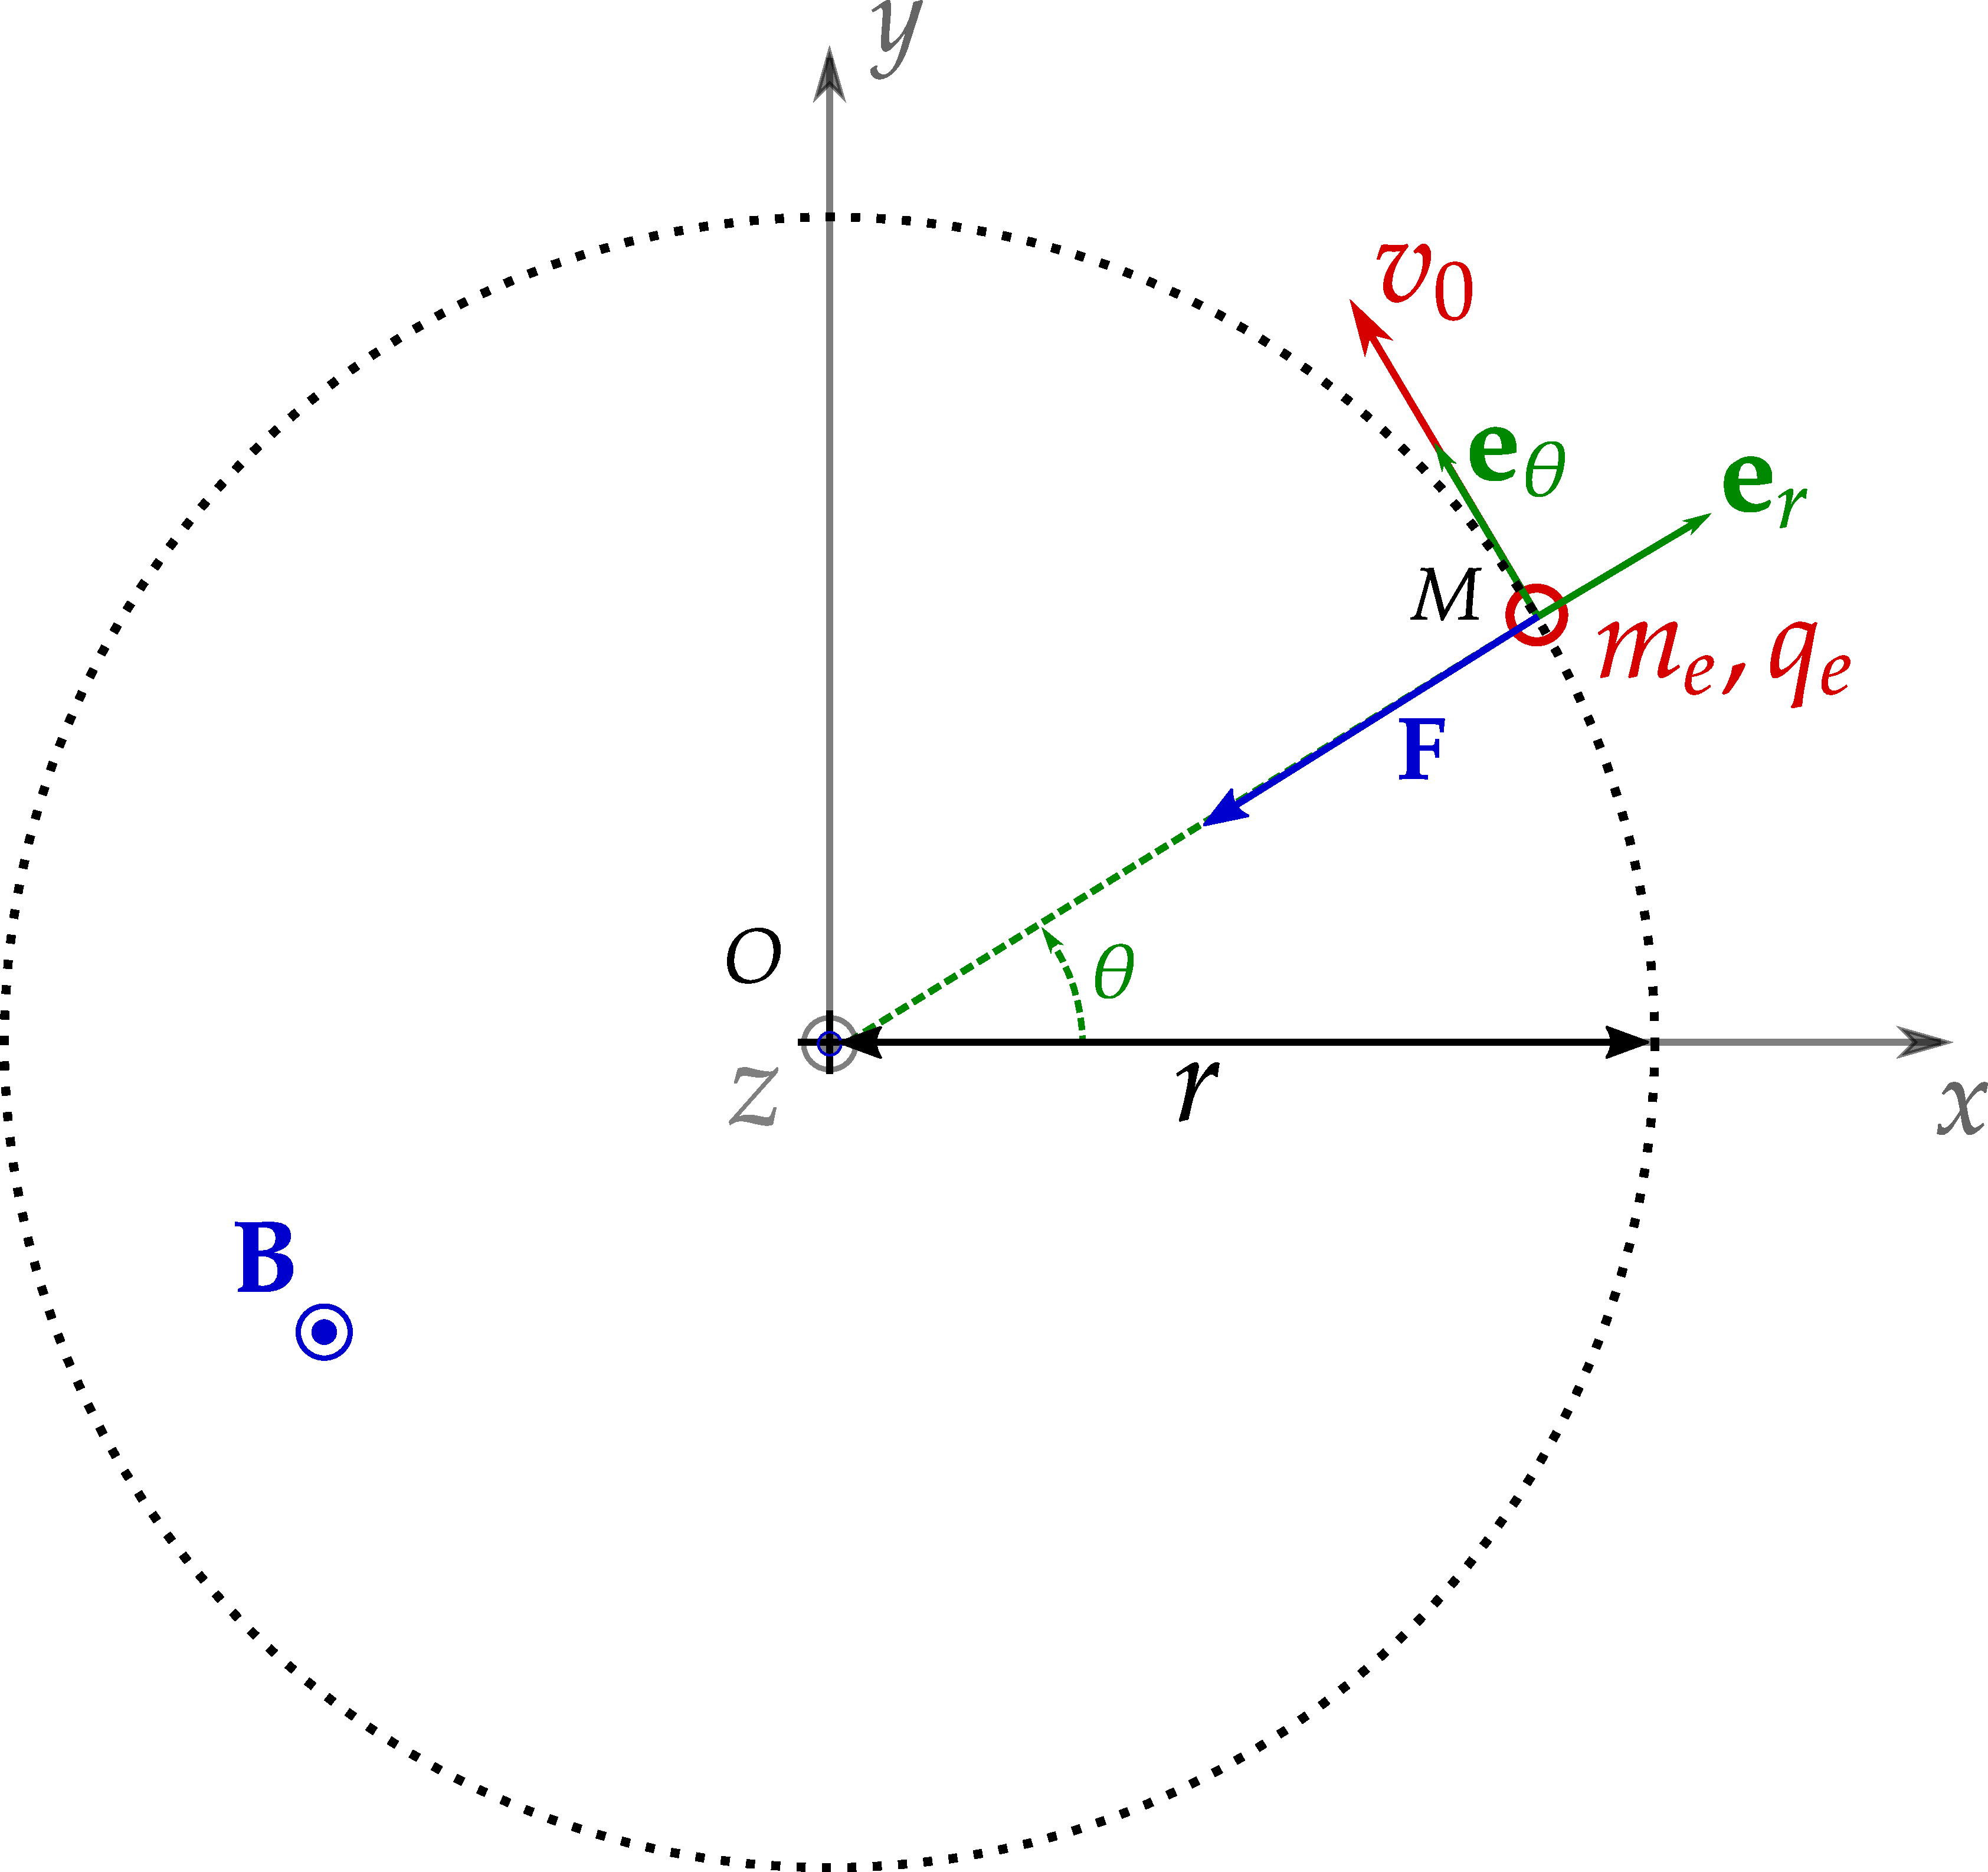
\includegraphics[scale=0.75]{cyclotron}
	\caption{Trajectoire d'un électron dans un champ magnétique uniforme.}%
	\label{fig:magneto_cyclotron}
\end{figure}

\section{La loi de Biot et Savart}
De la même manière que pour le champ électrostatique, nous
commençons par définir le champ magnétique généré par une charge ponctuelle. 
Soit une charge ponctuelle $q$ en un point $P$ de l'espace se déplaçant 
à la vitesse $\vecv$ dans le référentiel du laboratoire. Expérimentalement,
on observe que cette particule génère
en un point $M$ un champ magnétique $\vecb(M)$ tel que

\begin{equation*}
	\vecb(M) = \dfrac{\mu_0 q}{4 \pi} \vecv \wedge \dfrac{\mitbf{PM}}{||PM||^3},
\end{equation*}
où $\mu_0 = \unit{4 \pi \times 10^{-7}}{\tesla \usk \meter \usk \reciprocal 
\ampere}.$

\begin{figure}[h!]
	\centering
	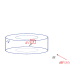
\includegraphics[]{biot_savart}
	\caption{Champ magnétique généré par un élément infinitésimal d'un conducteur
	de densité volumique de courant $\vecj$ en un point $M$ de l'espace.}%
	\label{fig:magneto_biot_savart}
\end{figure}

On considère un conducteur formant un volume $\mathcal{V}$ 
(voir Fig.~\ref{fig:magneto_biot_savart}) parcouru par des charges mobiles 
de densité volumique de charge $\rho$ se déplaçant à la vitesse $\vecv$. Un élément 
infinitésimal $\dV$ de ce circuit centré en $P$ génère en un point $M$ un champ magnétique

\begin{equation*}
	\mathrm{\textbf{d}}\mitbf{B}^P(M) = \dfrac{\mu_0 \rho(P) \dV}
	{4 \pi} \vecv(P) \wedge 
	          \dfrac{\mitbf{PM}}{||PM||^3},
\end{equation*}
où on reconnaît le vecteur densité de courant $\vecj(P) = \rho(P) \vecv(P)$. 
Le champ magnétique
$\vecb$ généré par l'ensemble du circuit en $M$ est alors obtenu en additionnant les 
contributions de chaque élément de ce dernier grâce au principe de superposition
\begin{equation*}
	\vecb(M) = \iiint_{P \in \mathcal{V}} \mathrm{\textbf{d}}\mitbf{B}^P(M)
		 = \iiint_{P \in \mathcal{V}} \dfrac{\mu_0}
		 {4 \pi} \vecj(P) \wedge 
	          \dfrac{\mitbf{PM}}{||PM||^3} \dV
\end{equation*}
On aboutit ainsi à la loi de Biot et Savart.

\begin{defn}[Loi de Biot et Savart]
	Le champ magnétostatique $\vecb(M)$ créé au point $M$ par une distribution
	volumique de courant $\vecj$ ($\ampere \usk \rpsquare \meter$) contenue
	dans un volume $\mathcal{V}$ est
	\begin{equation}
		\vecb(M) = \dfrac{\mu_0}{4 \pi} \iiint_{P \in \mathcal{V}} 
		\dfrac{\vecj(P) \wedge \mitbf{PM}}{||PM||^3} \dV,
	\end{equation}
	où $\mu_0 = \unit{4 \pi \times 10^{-7}}{\tesla \usk \meter \usk \reciprocal
	\ampere}$ est la perméabilité magnétique du vide.

\end{defn}

	Par un raisonnement similaire, on montre que pour une distribution 
	surfacique de courant $\vecj_s$ confinée sur une 
	surface $\mathcal{S}$, cette expression devient
	\begin{equation}
		\vecb(M) = \dfrac{\mu_0}{4 \pi} \iint_{P \in \mathcal{S}} 
		\dfrac{\vecj_s(P) \wedge \mitbf{PM}}{||PM||^3} \mathrm{d}S.
	\end{equation}

	Pour un circuit filiforme $\mathcal{C}$ parcouru par un courant $I$, 
	cette expression devient
	\begin{equation}
		\vecb(M) = \dfrac{\mu_0}{4 \pi} \int_{P \in \mathcal{C}} 
	\dfrac{I \dl \wedge \mitbf{PM}}{||PM||^3}.
	\end{equation}

\begin{exemple}
	On cherche à déterminer le champ magnétique généré par un fil infini $\mathcal{C}$
	parcouru
	par un courant d'intensité $I$ en un point $M$ 
	(voir Fig.~\ref{fig:magneto_spire}). On se place dans un repère cylindrique
	$(0, \er, \etheta, \ez)$. Les points $M$ et $P$ ont pour coordonnées 
	respectives $(r, \theta, 0)$ et $(0, 0, z_P)$.

	Le champ magnétique $\mathrm{\textbf{d}}\vecb^P(M)$ généré par un élément
	$\dl_P$ du fil centré en $P$ s'écrit
	\begin{equation*}
	\mathrm{\textbf{d}}\vecb^P(M) = \dfrac{\mu_0}{4 \pi} 
	              \dfrac{I \dl_P \wedge \mitbf{PM}}{||PM||^3},
	\end{equation*}
	où $\mitbf{PM} = \mitbf{PO} + \mitbf{OM} = - z_P\ez + r\er$. Dans un repère
	cylindrique, un élément infinitésimal $\dl_P$ du fil s'écrit
	$\dl_P = \dz_P \ez$. On a alors
	\begin{equation*}
		\dfrac{\dl_P \wedge \mitbf{PM}}{||PM||^3} = 
		\dfrac{r\dz_P}{||PM||^3}\etheta. 	
	\end{equation*}
	En remarquant que $||PM|| = r/\cos\alpha$, l'expression précédente devient alors
	\begin{equation*}
		\dfrac{r\dz_P}{||PM||^3}\etheta = \dfrac{\cos^3\alpha \dz_P}
		{r^2} \etheta
	\end{equation*}
	De même, on remarque que $z_p = r \tan\alpha$.
	Par différentiation, on obtient donc
	\begin{equation*}
		\dz_P = \mathrm{d}\left[r\tan\alpha\right] = 
		\dfrac{r \mathrm{d}\alpha}{\cos^2\alpha}.
	\end{equation*}
	Finalement,
	\begin{equation*}
		\mathrm{\textbf{d}}\vecb^P(M) = \dfrac{\mu_0 I \cos\alpha}
		{4 \pi r} \mathrm{d}\alpha \etheta.
	\end{equation*}
	Le champ $\vecb(M)$ généré au point $M$ par le fil s'obtient alors
	en utilisant le principe de superposition, ce qui revient à intégrer les champs 
	magnétiques infinitésimaux sur l'ensemble du fil. Pour parcourir l'ensemble du
	fil, $\alpha$ doit varier entre $-\pi/2$ et $\pi/2$. On a alors
	\begin{equation*}
		\boxed{\vecb(M) = \dfrac{\mu_0 I}{4\pi r}
			\times \displaystyle{\int_{-\pi/2}^{\pi/2} 
			\cos\alpha\mathrm{d}\alpha \etheta} =
	\dfrac{\mu_0 I}{2\pi r}\etheta.}
	\end{equation*}
	On obtient un champ magnétique porté par $\etheta$ et donc la norme ne dépend
	que de $r$. Les lignes de ce champ sont des cercles concentriques centrés
	sur le fil. $\vecb$ "tourne" autour du fil.
\end{exemple}
\begin{figure}[h!]
	\centering
	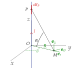
\includegraphics[scale=0.7]{fil}
	\caption{Champ magnétique créé en un point $M$ par un fil parcouru par
	un courant d'intensité $I$.}%
	\label{fig:magneto_spire}
\end{figure}

\begin{defn}[Calcul du champ magnétique par la loi de Biot et Savart]
	Comme nous l'avons vu dans l'exemple précédent, la loi de Biot et Savart
	peut s'avérer utile lorsqu'il s'agit de calculer le champ magnétique 
	$\vecb$ généré par une distribution de courant. Voici en résumé la démarche à suivre
	\begin{enumerate}
		\item Réaliser un schéma du système et choisir un repère adapaté.
		\item Exprimer le petit volume $\dV$, de surface $\mathrm{d}S$
		  ou de longueur $\dl$ dans ce système de coordonnées.
	  \item En multipliant cet élément par le courant ($\vecj$, $\vecj_s$ ou
	    $I$), on obtient le petit élément de courant associé.
	  \item Exprimer le vecteur $\mitbf{PM}$ dans le système de coordonnées
	    choisi.
    	\item En multipliant par $\dfrac{\mu_0}{4 \pi}$ et en faisant le produit 
	  vectoriel par $\dfrac{\mitbf{PM}}{||PM||^3}$, on fabrique le champ
	  élémentaire $\mathrm{\textbf{d}}\vecb^P(M)$ généré en $M$.
	\item Pour calculer $\vecb(M)$, il suffit alors d'intégrer sur la distribution
	  de courant.
	\end{enumerate}
\end{defn}
\section{Équation de la magnétostatique}
On considère un fil parcouru par un courant $I$ dans un
repère cylindrique $(O, \er, \etheta, \ez)$ (voir Fig.~\ref{fig:magneto_spire}). 
Comme vu ci-dessus, le champ
magnétique créé par ce fil en un point $M$ situé à une distance $r$ du fil
est donné par
\begin{equation*}
	\vecb(M) = \dfrac{\mu_0 I}{2 \pi r}\etheta.
\end{equation*}
Comme pour le champ électrostatique, nous allons nous servir de cet exemple simple 
pour retrouver certaines propriétés du champ magnétostatique.

\subsection{Le théorème d'Ampère}
Le théorème d'Ampère est l'équivalent pour le champ magnétostatique $\vecb$
du théorème de Gauss. Il va nous permettre de calculer facilement le champ
magnétostatique généré par une distribution de courants simple.

Les lignes du champ $\vecb$ créé par le fil sont des cercles dont l'axe est le
fil. Nous cherchons donc dans un premier temps à calculer la circulation de $\vecb$ 
sur la ligne de champ $\mathcal{C}$ de rayon $r$ passant par $M$. 
On a bien pris soin au préalable
d'orienter cette dernière. Dans un repère cylindrique, un petit élément $\dl$ de ce 
contour fermé s'écrit $\dl = r \dtheta \etheta$. La circulation de $\vecb$ sur
ce contour s'écrit donc
\begin{equation*}
	\boxed{\displaystyle{\oint_\mathcal{C} \vecb \cdot \dl = 
		\oint_0^{2 \pi} \dfrac{\mu_0 I}{2 \pi r} r\dtheta
	= \mu_0 I.}}
\end{equation*}
On constate que la circulation du champ $\vecb$ le long du circuit $\mathcal{C}$
ne dépend que du courant $I$ que ce dernier enlace. Cette propriété que nous venons
de montrer pour un fil est en fait une propriété générale du champ magnétostatique.

\begin{defn}[Théorème d'Ampère]
	La circulation du champ magnétostatique $\vecb$ le long d'un circuit fermé
	$\mathcal{C}$ est égale au courant \textbf{algébrique} $I_\mathrm{int}$ 
	enlacé par ce dernier multiplié
	par $\mu_0$
	\begin{equation}
		\oint_\mathcal{C} \vecb \cdot \dl = \mu_0 I_\mathrm{int}.
	\end{equation}
	Le contour sur lequel est réalisée l'intégrale est appelé contour d'Ampère.
	Le courant enlacé $I_\mathrm{int}$ est le courant qui traverse une surface 
	orientée
	qui s'appuie sur le contour d'Ampère. L'orientation de la surface 
	se déduit de celle du contour
	grâce à la règle de la main droite ou du tire-bouchon.
\end{defn}

\begin{exemple}
	\begin{minipage}{0.6\linewidth}
	Soit deux fils électriques parcourus par des courants $I_1$ et $I_2$.
	Avec les orientations choisies, le théorème d'Ampère appliqué au 
	contour $\mathcal{C}$ s'écrit
	\begin{equation*}
		\oint_\mathcal{C} \vecb \cdot \dl = \mu_0(I_1 - I_2).
	\end{equation*}
	\end{minipage}
	\hfill
	\begin{minipage}{0.35\linewidth}
		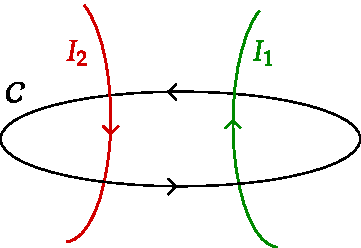
\includegraphics[width=0.8\linewidth]{ampere_ex}
	\end{minipage}

\end{exemple}

Le théorème d'Ampère peut-être traduit sous une forme locale:
appelée \textbf{équation de Maxwell-Ampère}, qui relie alors le champ magnétostatique
au vecteur densité de courant.

\begin{defn}[Équation de Maxwell-Ampère]
	L'équation de Maxwell-Ampère relie le champ magnétostatique $\vecb$
	au vecteur densité de courant $\vecj$
	\begin{equation}
		\rot \vecb = \mu_0 \vecj.
		\label{eq:magneto_ma}
	\end{equation}
	Cette équation est une relation $\textbf{locale}$, elle permet de relier 
	les dérivées spatiales du champ $\vecb$ en un point de l'espace au vecteur
	$\vecj$ en ce même point.
\end{defn}

\subsection{Flux du champ magnétostatique $\vecb$}
On cherche maintenant à calculer la divergence du champ $\vecb$. En coordonnées 
cylindriques, cela donne
\begin{equation*}
	\div \vecb = \dfrac{1}{r}\left(\dd{r B_r}{r} + \dd{B_\theta}{\theta} \right)
	+ \dd{B_z}{z},
\end{equation*}
où $B_r$, $B_\theta$ et $B_z$ sont les composantes de $\vecb$. 
Dans le cas du fil infini, $B_\theta$ est la seule composante non nulle de $\vecb$ 
et elle ne dépend pas
de $\theta$. On a donc
\begin{equation*}
	\div \vecb = 0.
\end{equation*}
Ce résultat se généralise à un champ magnétostatique $\vecb$ quelconque sous
la forme de l'équation de Maxwell-Thomson.

\begin{defn}[Équation de Maxwell-Thomson]
	Un champ magnétique $\vecb$ vérifie toujours
	\begin{equation*}
		\div \vecb = 0.
	\end{equation*}
	Cette relation locale est vérifiée en tout point de l'espace.
\end{defn}

\begin{rem}
La divergence de $\vecb$ étant nulle, l'analyse vectorielle affirme
qu'il est possible dans ce cas de définir un champ vectoriel $\veca$,
défini à un gradient près, tel que $\rot \veca = \vecb$,
appelé le potentiel vecteur.
\end{rem}

Comme l'équation de Maxwell-Ampère, cette équation peut se mettre sous une forme
intégrale, en exprimant le flux du champ magnétique à travers une surface fermée
$\mathcal{S}$.

\begin{defn}[Flux du champ magnétostatique]
	Le flux du champ magnétique $\vecb$ à travers une surface fermée 
	$\mathcal{S}$ est nul
	\begin{equation*}
		\oiint_\mathcal{S} \vecb \cdot \ds = 0.
	\end{equation*}
	On dit que le champ $\vecb$ est à flux conservatif.
\end{defn}

	\begin{minipage}{0.6\linewidth}
	On peut appliquer ce résultat à une surface $\mathcal{S}$ particulière
	constituée d'une portion de tube de champ de section d'entrée $\mathcal{S}_e$,
	de section de sortie $\mathcal{S}_s$ et de section latérale $
	\mathcal{S}_l$. 	
	\end{minipage}
	\hfill
	\begin{minipage}{0.3\linewidth}
	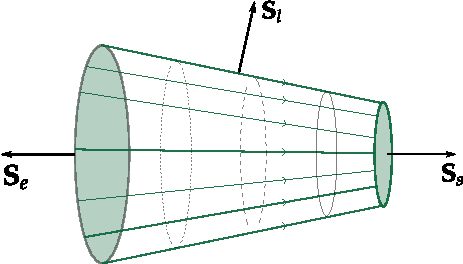
\includegraphics[scale=0.7]{tube}
	\end{minipage}
	\vspace{0.5cm}

\begin{defn}[Tube de champ]
	L'ensemble des lignes de champ s'appuyant sur un contour fermé forme un 
	tube de champ.
\end{defn}
	
	D'après le théorème d'Ampère la flux de $\vecb$ à
	travers cette surface est nul.
	Par définition du tube de champ, l'intégrale sur la surface 
	latérale est nulle. Il reste donc 
	\begin{equation*}
		\iint_\mathcal{S_e} \vecb \cdot \ds_e =
		- \iint_\mathcal{S_s} \vecb \cdot \ds_s 
		\iff
		\displaystyle{\left\lvert\iint_\mathcal{S_e} \vecb \cdot \ds_e\right\rvert =
		\left\lvert\iint_\mathcal{S_s} \vecb \cdot \ds_s\right\rvert}.
	\end{equation*}
	Le flux entrant dans la surface est égal au flux sortant de cette dernière.
	De plus, la surface de sortie étant de taille plus importante que 
	la surface d'entrée, on en conclut que le champ est plus intense
	à l'entrée du tube qu'à la sortie. Le champ $\vecb$ étant à flux
	conservatif, un resserrement des lignes de champs traduit une augmentation
	de l'intensité de ce dernier.

\begin{defn}[Flux conservatif et lignes de champ]
	Le champ magnétique étant à flux conservatif, ses lignes de champs
	se resserrent dans les zones de forte intensité. Inversement, ces dernières
	s'éloignent lorsqu'il devient plus faible
\end{defn}

\section{Étude des lignes de champ de \vecb}
Nous nous intéressons dans cette partie aux propriétés spatiales du champ $\vecb$.
Nous allons voir comment les \textbf{lignes de champ} nous renseignent sur sa répartition 
dans l'espace.

Nous nous intéressons au champ magnétique produit par un solénoïde 
(voir Fig.~\ref{fig:magneto_solenoide}).
Les lignes de champ nous permettent de retrouver quelques propriétés du champ 
magnétostatique énoncées précédemment.

\begin{figure}[htpb]
	\centering
	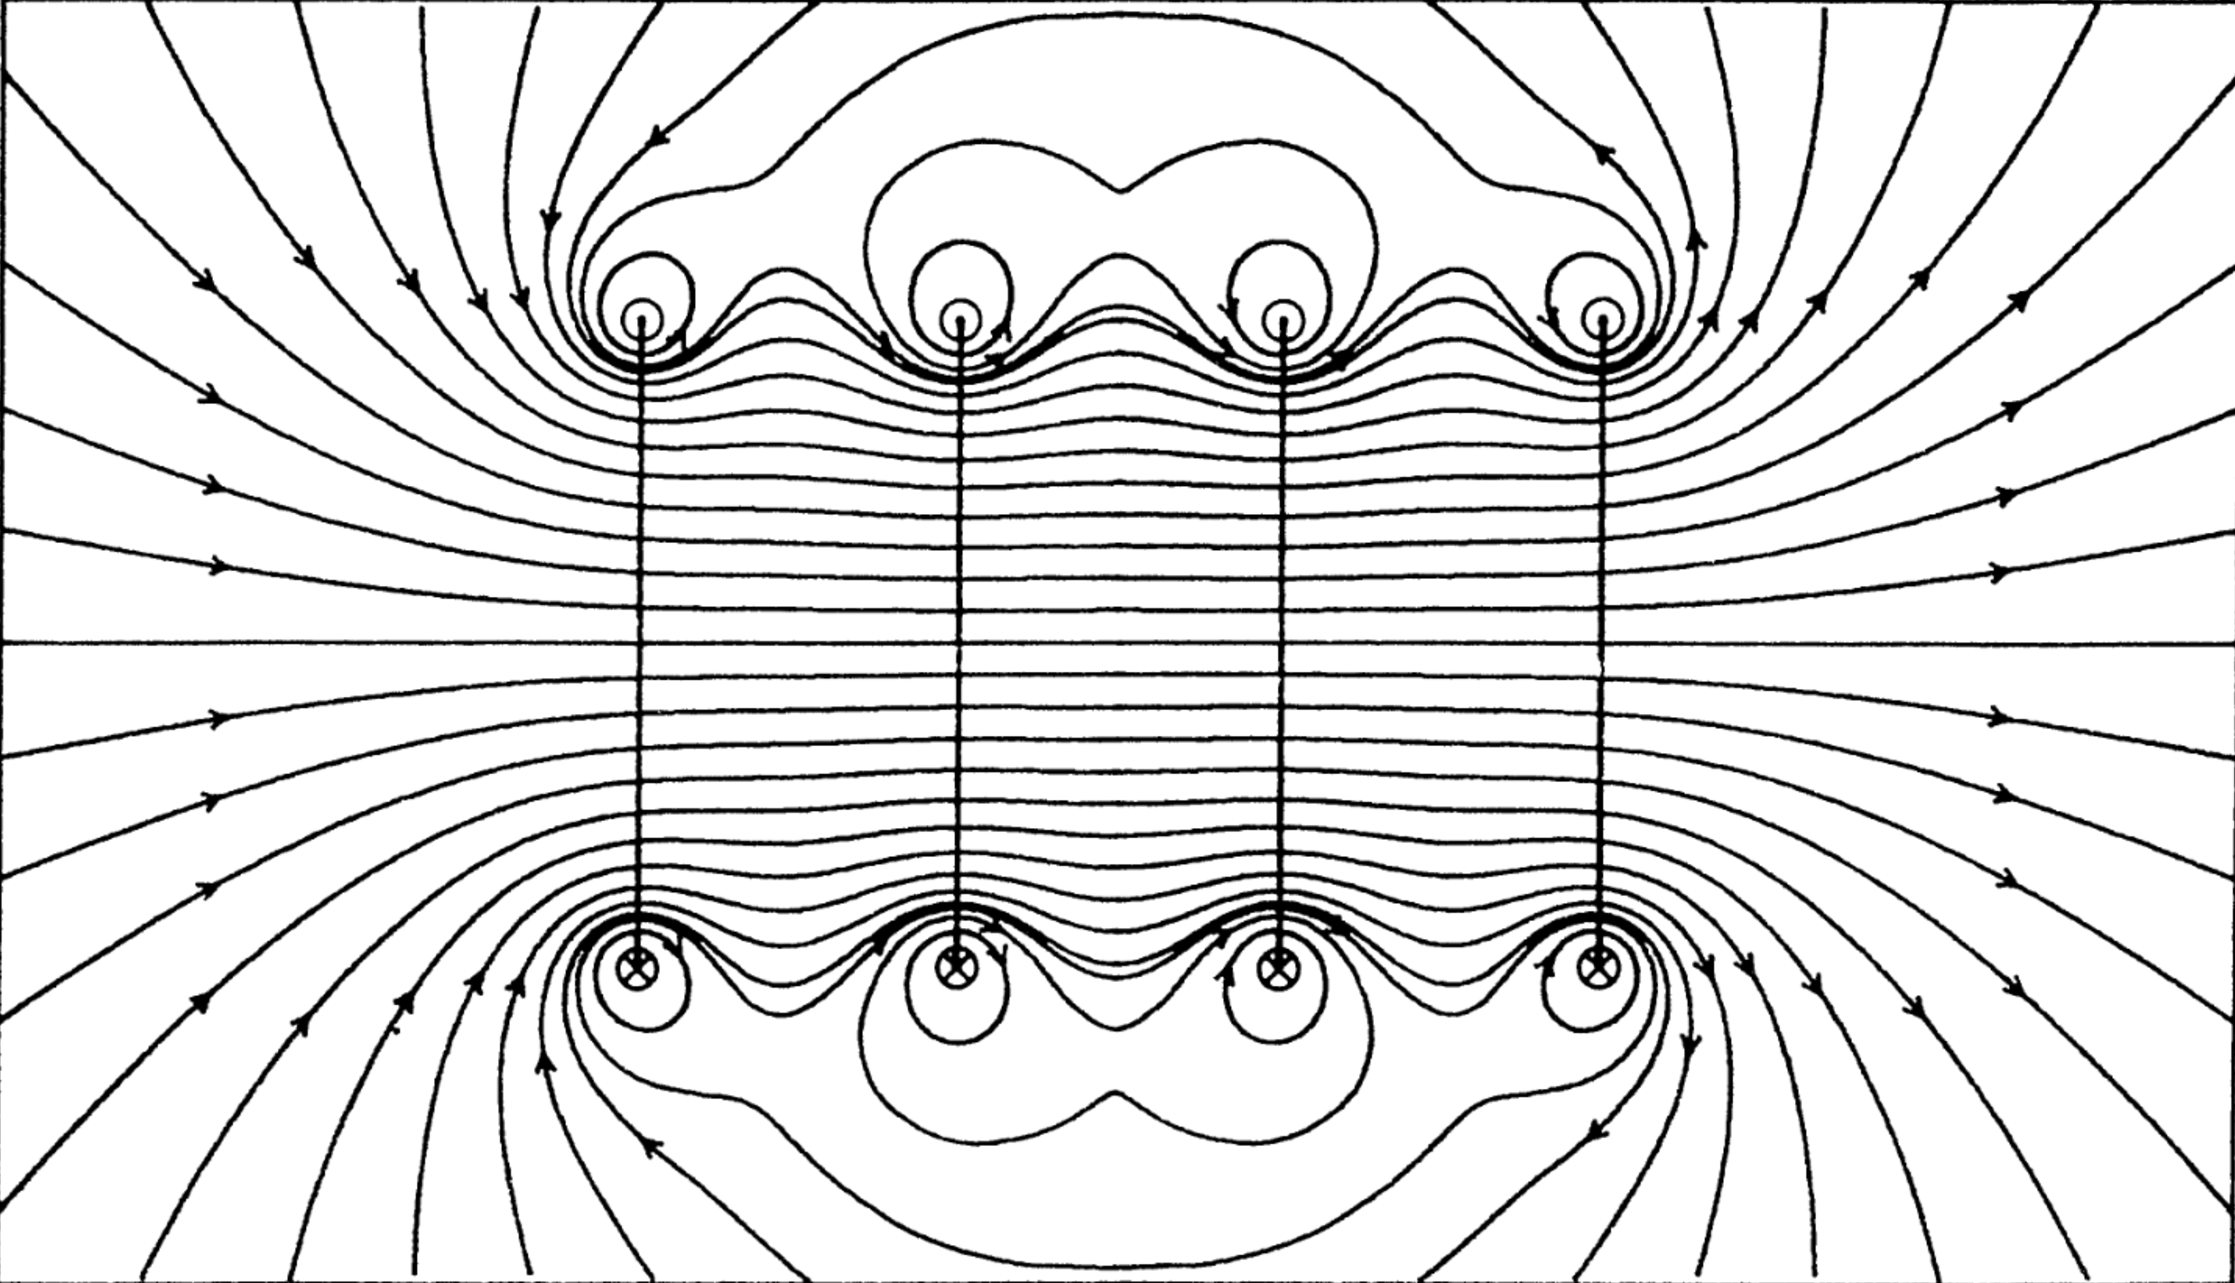
\includegraphics[width=0.7\linewidth]{solenoide}
	\caption{Lignes du champ magnétique généré par un solénoïde constitué de
		4 bobines parcourues dans le même sens par la même intensité.
		Cette figure est extraite de \cite{Gie1985}}%
	\label{fig:magneto_solenoide}
\end{figure}

\begin{enumerate}
	\item On remarque tout d'abord que les lignes de champ 
	  sont des contours fermés qui entourent les fils parcourus par un courant.
	  Cette première observation est une conséquence directe de l'équation
	  de Maxwell-Ampère. L'orientation de ces lignes de champ s'obtient
	  d'ailleurs en considérant le sens du courant dans les fils et en utilisant
	  la règle de la main droite.
      \item La divergence nulle de $\vecb$ est aussi visible sur cette carte de 
	champ. En effet, on constate que les lignes de champ ne convergent/divergent
	pas en un point de l'espace, contrairement au champ électrostatique.
      \item Dans le cas du champ magnétique, le resserrement des lignes de champ
	traduit une augmentation de la norme de ce dernier. On conclut que le champ
	est plus intense à l'intérieur du solénoïde qu'à l'extérieur. De plus, les
	lignes de champ étant parallèles à l'intérieur du solénoïde, on conclut que
	le champ est uniforme.
      \item Grâce aux lignes de champ, on retrouve rapidement les plans de 
	  symétrie et d'antisymétrie du champ magnétique. Le plan médiateur 
	  du solénoïde est par exemple un plan de symétrie du champ magnétique. 
          L'analyse de ces symétries sera utile pour calculer le champ
          magnétique résultant d'une distribution de courant.
\end{enumerate}

\section{Calcul du champ magnétostatique}
\label{sec:calcul_e}
Nous allons voir dans cette partie comment nous pouvons utiliser le théorème d'Ampère
pour calculer le champ magnétostatique $\vecb$ créé 
par une distribution de courants simple. Nous nous intéressons ici à une bobine
torique constituée d'un fil régulièrement bobiné autour d'un tore de section
carré (voir Fig.~\ref{fig:magneto_tore}). Cette bobine est caractérisée par le nombre $N$
total de spires bobinés, son rayon intérieur $R$ 
et sa hauteur $h$. La bobine est parcourue par un courant $I$.

On cherche à déterminer 
l'expression du champ électrique $\vecb$ en un point $M$ de l'espace. Pour ce faire, 
il suffit de suivre le mode d'emploi suivant
\begin{enumerate}
	\item Faire un schéma du système ! C'est absolument indispensable
	  (voir Fig.~\ref{fig:magneto_tore})
	\item Choisir un repère adapté au problème
	\item Étudier les invariances de cette distribution
	\item Étudier les symétries de la distribution de courants à l'origine 
	  du champ magnétostatique
	\item Choisir un contour d'Ampère et appliquer le théorème d'Ampère.
\end{enumerate}

Au vu de la géométrie du système, nous choisissons ici d'utiliser 
un repère cylindrique $(O, \er, \etheta, \ez)$.
Le point $M$ est donc repéré par ses coordonnées $(r, \theta, z)$. Le champ
magnétostatique en $M$ s'écrit de manière générale

\begin{equation}
	\vecb(M) = B_r(M)\er + B_\theta(M)\etheta + B_\varphi(M)\ephi.
	\label{eq:tore}
\end{equation}
Le champ magnétostatique est un vecteur à trois composantes et chaque composante
dépend des coordonnées de $M$. Pour simplifier cette expression, il est intéressant
de considérer les invariances et symétries de la distribution de courant qui génère
le champ $\vecb$.

\begin{figure}
	\centering
	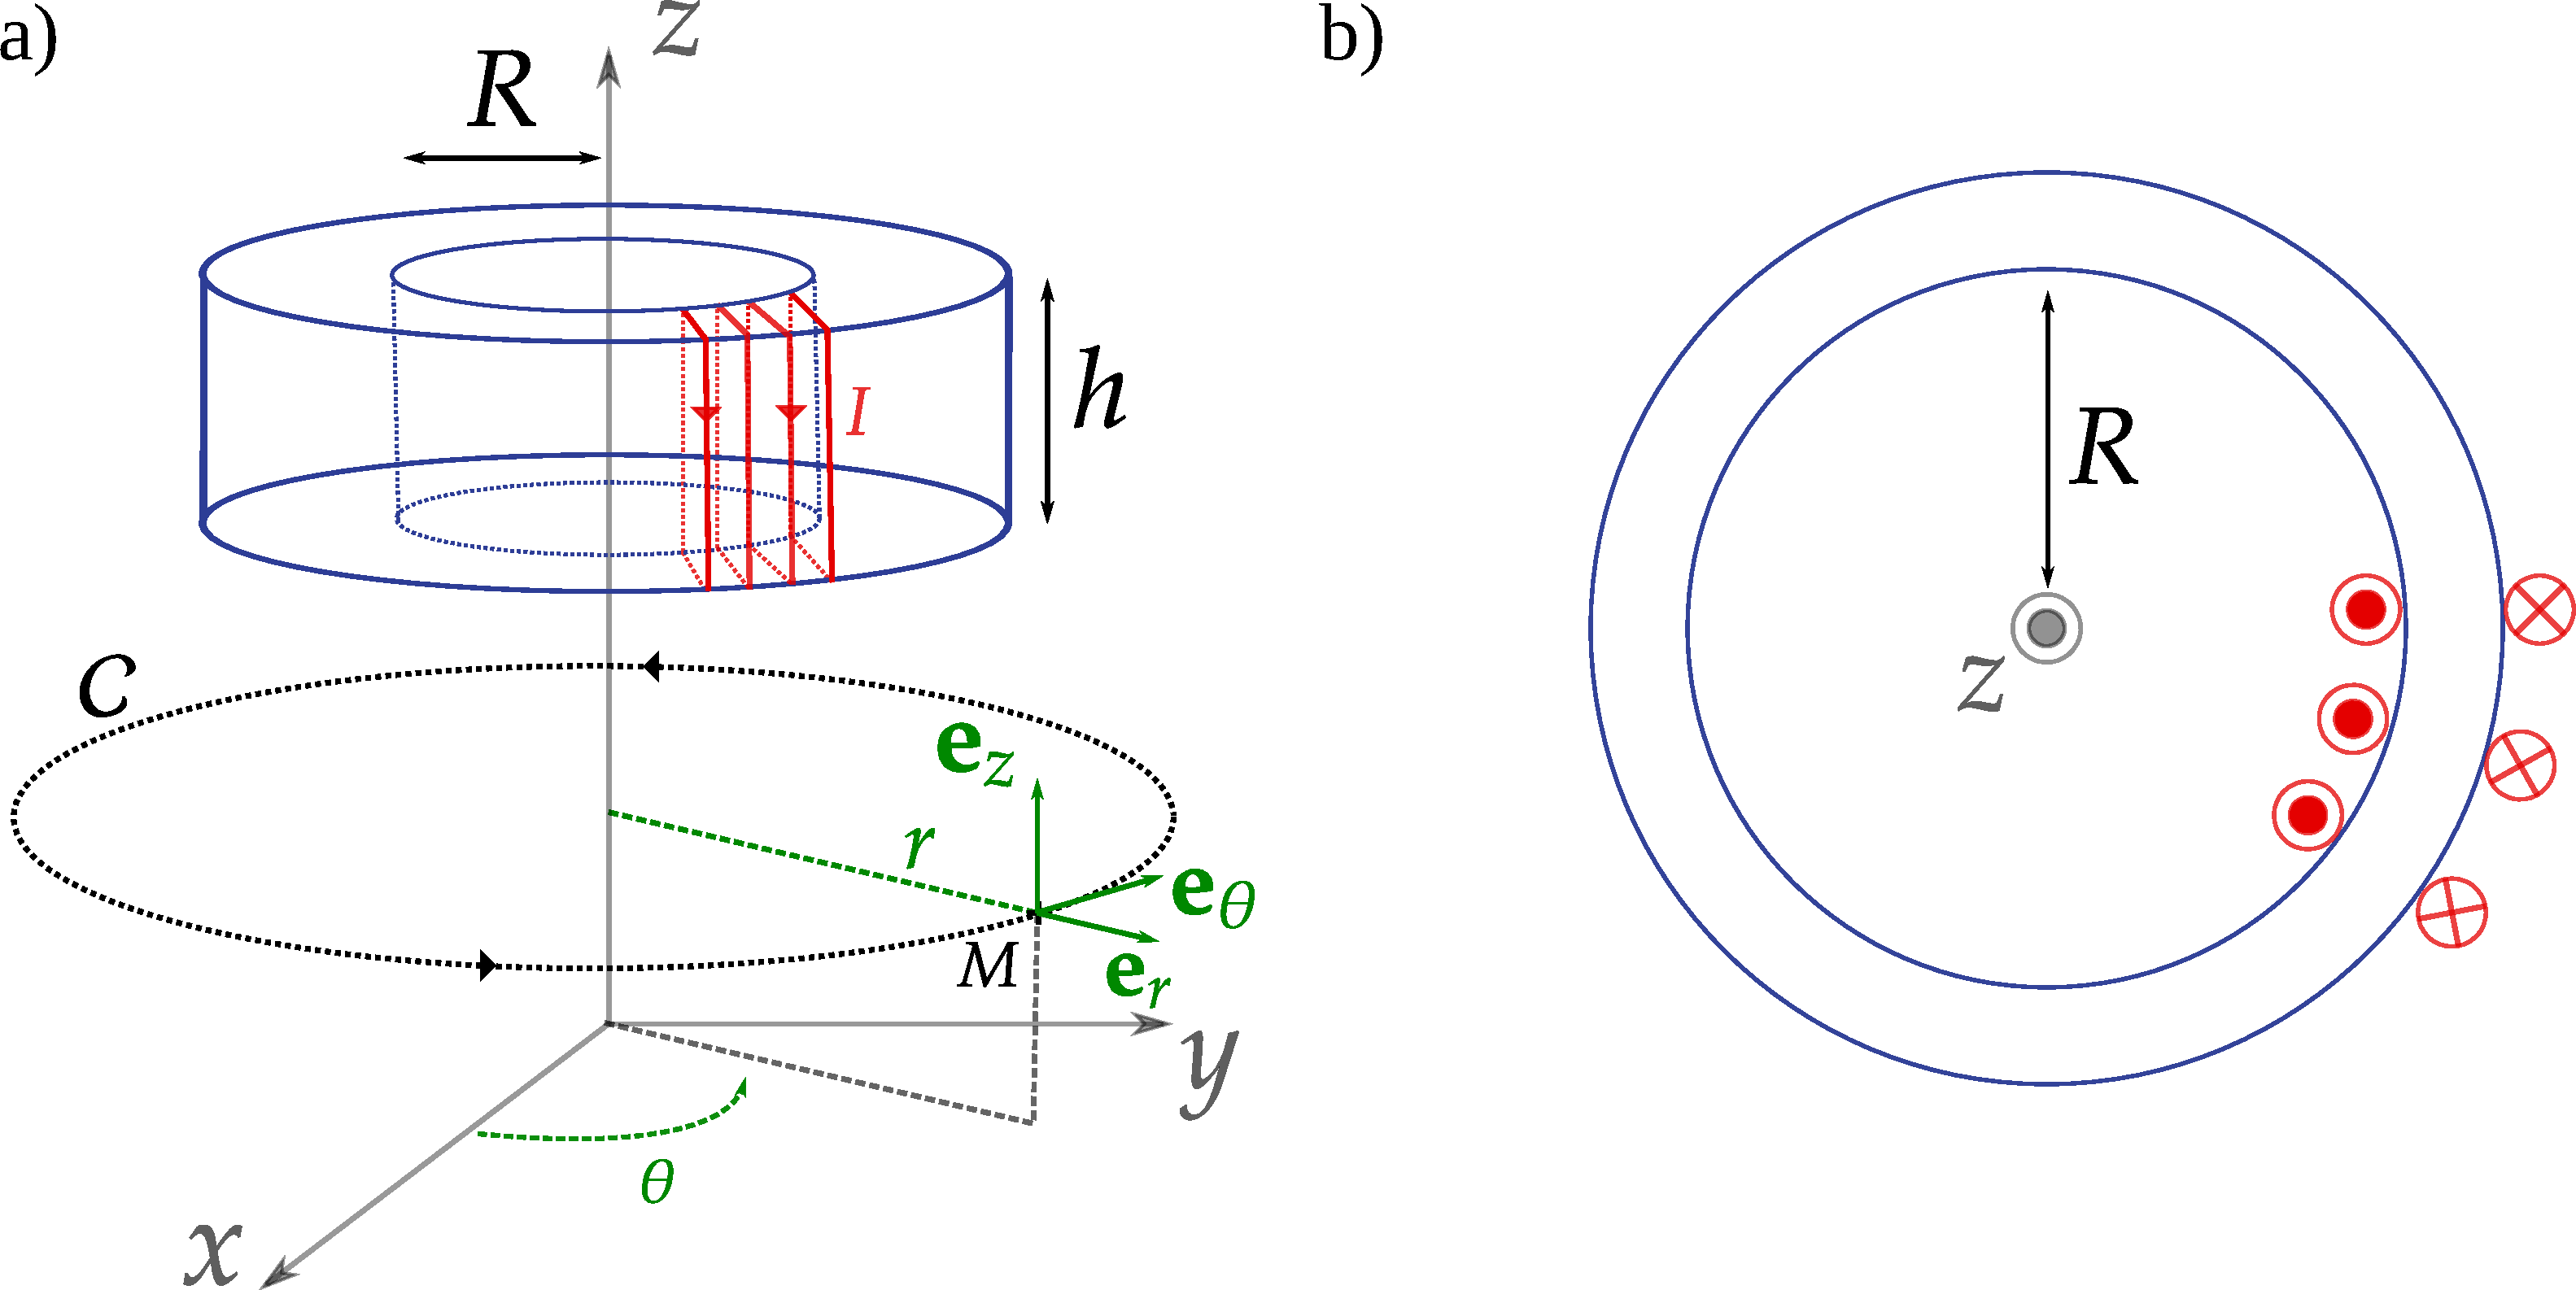
\includegraphics[scale=1]{tore}
	\caption{Bobine torique à gauche et coupe perpendiculaire à $(Oz)$
	de cette bobine à droite.}%
	\label{fig:magneto_tore}
\end{figure}

\subsection{Invariance de la distribution de courants}
On cherche ici à savoir si la distribution de courant est modifiée sous l'effet
d'une translation ou d'une rotation de l'espace. En d'autres termes, on regarde
de quelles variables elle dépend. Étant donné que les spires sont uniformément
répartie sur le tore, on observe que

\begin{itemize}
	\item  si je tourne le tore d'un angle $\Delta \theta$ dans la
	  direction $\etheta$, le problème
	  ne change pas. La distribution de courant est donc invariante 
	  par rotation selon l'angle $\theta$. $\vecb$ \textbf{ne dépend pas de
	  $\mitbf{\theta}$}.
\end{itemize}

Finalement, l'expression~\ref{eq:tore} du champ magnétique se simplifie donc en 

\begin{equation*}
	\boxed{\vecb(M) = B_r(r,z)\er + B_\theta(r,z)\etheta + B_z(r,z)\ez.}
\end{equation*}
\subsection{Symétries de la distribution de courants}

Si on applique ce principe au champ magnétique créé par une distribution 
de courants, cela revient à dire que les symétries de la distributions de 
courants doivent se retrouver dans les symétries du champ magnétique. On en 
déduit les règles suivantes

\begin{defn}[Symétries de $\vecb$ et de la distribution de courant]
\begin{itemize}
  \item si $(\Pi)$ est un plan d'antisymétrie de la distribution de courant et que 
    $M$ appartient à $(\Pi)$, alors obligatoirement $\vecb(M)$ doit 
    appartenir à $(\Pi)$,
  \item si $(\Pi)$ est un plan de symétrie de la distribution de courant 
    et que $M$ appartient à $(\Pi)$, alors obligatoirement $\vecb(M)$ doit 
    être orthogonal à $(\Pi)$.
\end{itemize}
\end{defn}

\begin{rem}
	Le champ magnétostatique $\vecb$ appartient aux plans d'\textbf{antisymétrie}
	de la distribution de courant et non aux plans de symétrie comme
	c'est le cas pour le champ électrostatique. Le vecteur $\vecb$ est 
	qualifié de vecteur axial.
\end{rem}

Pour appliquer ces règles à notre exemple, on détermine les plans de symétrie 
et d'antisymétrie de la distribution de courants auquels 
le point $M$ appartient

\begin{itemize}
	\item le plan $(M, \er, \ez)$ est un plan de symétrie de la distribution
	  de courant. $\vecb(M)$ \textbf{doit être orthogonal à ce plan}.
\end{itemize}

$\vecb(M)$ doit être orthogonal au plan $(M, \er, \ez)$, 
il doit donc être colinéaire à $\etheta$

\begin{framed}
\begin{equation*}
	\vecb(M) = B_\theta(r, z) \etheta.
\end{equation*}
\end{framed}

Nous n'avons imposé aucune condition sur la position de $M$, cette relation est
donc vraie pour tout point $M$ de l'espace. Maintenant que l'expression du 
champ magnétique a été simplifiée au maximum, on cherche à appliquer le théorème
d'Ampère.

\subsection{Application du théorème d'Ampère}
La distribution de courant présente une symétrie de révolution. On choisit comme contour 
d'Ampère un cercle $\mathcal{C}$ de rayon $r$, de centre $O$ et orienté
dans le sens de $\etheta$ qui passe par $M$ 
(voir Fig~\ref{fig:magneto_tore}) et on applique le théorème d'Ampère à ce dernier

\begin{equation*}
	\oint_\mathcal{S} \vecb(M) \cdot \dl = \mu_0 I_\mathrm{int},
	\label{eq:cavite_gauss}
\end{equation*}
où $I_\mathrm{int}$ est la courant enlacé par $\mathcal{C}$. On commence
par déterminer l'expression du membre de gauche. Dans un repère cylindrique,

\begin{equation*}
	\dl = r \dtheta \etheta.
\end{equation*}
On obtient alors
\begin{equation*}
	\oint_\mathcal{C} \vecb(M) \cdot \dl = 
	\oint_\mathcal{C} B(r,z) \etheta \cdot r \dtheta \etheta
	= B(r, z) r \int_0^{2 \pi} \dtheta
	= 2 \pi r B(r,z).
\end{equation*}
On s'intéresse maintenant au terme de droite de l'équation.
Deux cas de figure se présentent:
\begin{itemize}
	\item $M$ est situé dans le tore: le courant enlancé par $\mathcal{C}$ est alors
	  $I_\mathrm{int} = NI$.
       \item $M$ est situé à l'extérieur du tore: le courant enlacé par 
	       $\mathcal{C}$ est donc nul. Soit parce que le contour n'enlace 
	       aucun courant, soit parce qu'il enlace autant de courants positifs
	       que de courants négatifs.
\end{itemize}
Finalement,
\begin{framed}
\begin{itemize}
	\item si $M$ se trouve à l'intérieur du tore, 
	  $\vecb(M) = \dfrac{\mu_0 N I}{2 \pi r} \etheta$.
	\vspace{1em}
\item si $M$ est en dehors du tore, $\vecb(M) = \mitbf{0}$. 
\end{itemize}
\end{framed}
%\nocite{*}
%\putbib[magnetostatique]

%\newpage

%\chapter{Magnétostatique}
\label{chap:magnetostatique}
\section*{Objectifs}%
\label{sec:objectifs}
\begin{itemize}
	\item Connaître les équations qui contrôlent l'évolution spatiale 
	  du champ magnétostatique $\vecb$.
	\item Faire le lien entre ces équations et une carte de champ 
	  magnétique.
	\item Savoir calculer le champ magnétostatique résultant d'une 
	  distribution simple de courants.
\end{itemize}
\newpage
\section*{Introduction}
La magnétostatique étudie les champs magnétiques créés par des courants permanents.
Le plus souvent, on cherche alors à déterminer le champ magnétostatique $\vecb$
qui résulte d'une distribution de courant $\vecj$ connue. Nous nous intéressons
dans ce chapitre au champ magnétique créé par des courants circulants 
dans des conducteurs. Les milieux aimantés seront abordés plus loin dans le cours.

\section{La force de Lorentz}%
L'interaction entre deux particules immobiles a permis de définir la force de 
Coulomb dans le chapitre~\ref{chap:electrostatique}. Cette interaction 
électrostatique ne suffit plus lorsqu'il s'agit de décrire la dynamique de 
charges en mouvement. En 1895, le physicien néerlandais Hendrick Antoon Lorentz
propose alors l'ajout d'un second terme à la force coulombienne qui fait apparaître
la champ magnétostatique $\vecb$. 

\begin{defn}[Champ magnétostatique]
	Au même titre que le champ électrostatique, le champ magnétique $\vecb$
	est un champ vectoriel. Il est généré par une distribution de courant ou 
	par un aimant. Il s'exprime en tesla, noté $\tesla$ ($\kilogram \usk
	\rpsquare \second \reciprocal \ampere$ en SI). On rappelle quelques ordres de
	grandeur du champ magnétique
	
	\begin{center}
	\begin{tabular}{l|l}
		\textbf{Dispositif} 	& $\vecb (\tesla)$ \\ \hline
		Champ magnétique terrestre à la surface & $47 \times 10^{-6}$ \\
		Champ créé à $\unit{1}{\centi \meter}$ d'un fil parcouru par 
		un courant de $\unit{10}{\ampere}$
								 & $2 \times 10^{-5}$ \\
		Champ créé à $\unit{1}{\milli \meter}$ d'un aimant permanent& $0.1 - 1$ \\
		Électroaimant & $10 - 100$ \\
		Étoile à neutrons en surface & $10^{11}$\\
	\end{tabular}
	\end{center}
Le champ magnétique vérifie lui aussi le principe de superposition.
\end{defn}

\begin{defn}[Force de Lorentz]
Une particule de charge $q$ se déplaçant à la vitesse $\vecv$ dans un champ magnétique
$\vecb$, subit une force appelée force de Lorentz
\begin{equation}
	\vecf = q\vecv \wedge \vecb.
\end{equation}
Cette force est donc toujours orthogonale à la vitesse de la particule.
Contrairement à la force électrostatique, la force magnétique n'entraîne donc pas 
de variation de la vitesse de la particule, elle permet seulement de dévier sa 
trajectoire. En effet, la puissance magnétique $\mathcal{P}$ vaut
\begin{equation*}
	\mathcal{P} = \vecf \cdot \vecv = (q\vecv \wedge \vecb) \cdot \vecv = 0.
\end{equation*}
La force magnétique ne permet donc pas de mettre une particule chargée en mouvement.
\end{defn}

Comme pour la force électrostatique, le poids d'une particule chargée est bien souvent 
négligeable devant celui de la force de Lorentz. Pour illustrer cela, prenons le 
cas d'un électron de masse $m_e = \unit{9.1 \times 10^{-31}}{\kilogram}$ et de
charge $q = \unit{1.6 \times 10^{-19}}{\coulomb}$ se déplaçant à une vitesse
$v = \unit{10^5}{\meter \usk \reciprocal \second}$ dans un champ magnétique uniforme
$B = \unit{1}{\tesla}$. On trouve alors
\begin{equation*}
	\dfrac{mg}{qvB} \approx 10^{-15}.
\end{equation*}
On peut alors toujours négliger le poids d'une particule chargée
devant la force de Lorentz.

\begin{exemple}
	On s'intéresse ici au mouvement d'un électron de charge $-e$ et de 
	masse $m$ dans un 
	champ magnétique uniforme $\vecb$ (voir Fig.~\ref{fig:magneto_cyclotron}). 
	La vitesse initiale $\vecv_0$ de la particule est orthogonale au champ
	$\vecb$. La particule est donc soumise à la force de Lorentz et à son
	poids que nous négligeons ici. 
	
	Expérimentalement, on constate que la trajectoire 
	de la particule est circulaire. La force de Lorentz ne travaillant pas, 
	la norme de la vitesse reste en tout temps égale à $v_0$. Le mouvement de la 
	particule est donc uniforme et circulaire.
	
	On se place dans
	un référentiel polaire $(O, \er, \etheta)$. La position de la particule
	est donc repérée par ses coordonnées $(r, \theta)$. L'application du principe
	fondamental de la dynamique à la particule dans le référentiel du
	laboratoire supposé galiléen donne
	\begin{equation*}
		m \dot{\vecv} = q \vecv \wedge \vecb,
	\end{equation*}
	où la notation $\dot{v}$ est utilisée pour la dérivée temporelle.
	Dans un référentiel polaire et pour un mouvement circulaire uniforme, 
	$\vecv = r\dot{\theta} \etheta = v_0 \etheta$ 
	et $\dot{\vecv} = - v_0^2/r\er$. On obtient donc
	\begin{equation*}
		m \dfrac{v_0^2}{r}\er = -e v_0 \etheta \wedge \ez =e v_0 B \er \iff 
		\dot{\theta} = \dfrac{eB}{m}
	\end{equation*}
	L'électron suit donc un mouvement circulaire uniforme à la vitesse angulaire
	$eB/m$ appelée pulsation cyclotron. Dans le cyclotron de University of Michigan,
	le champ magnétique vaut $B = \unit{0.10}{\tesla}$, ce qui donne une pulsation de 
	$\unit{1.7 \times 10^{10}}{\rad \usk \reciprocal \second}$ pour un électron.

\end{exemple}
\begin{figure}[h!]
	\centering
	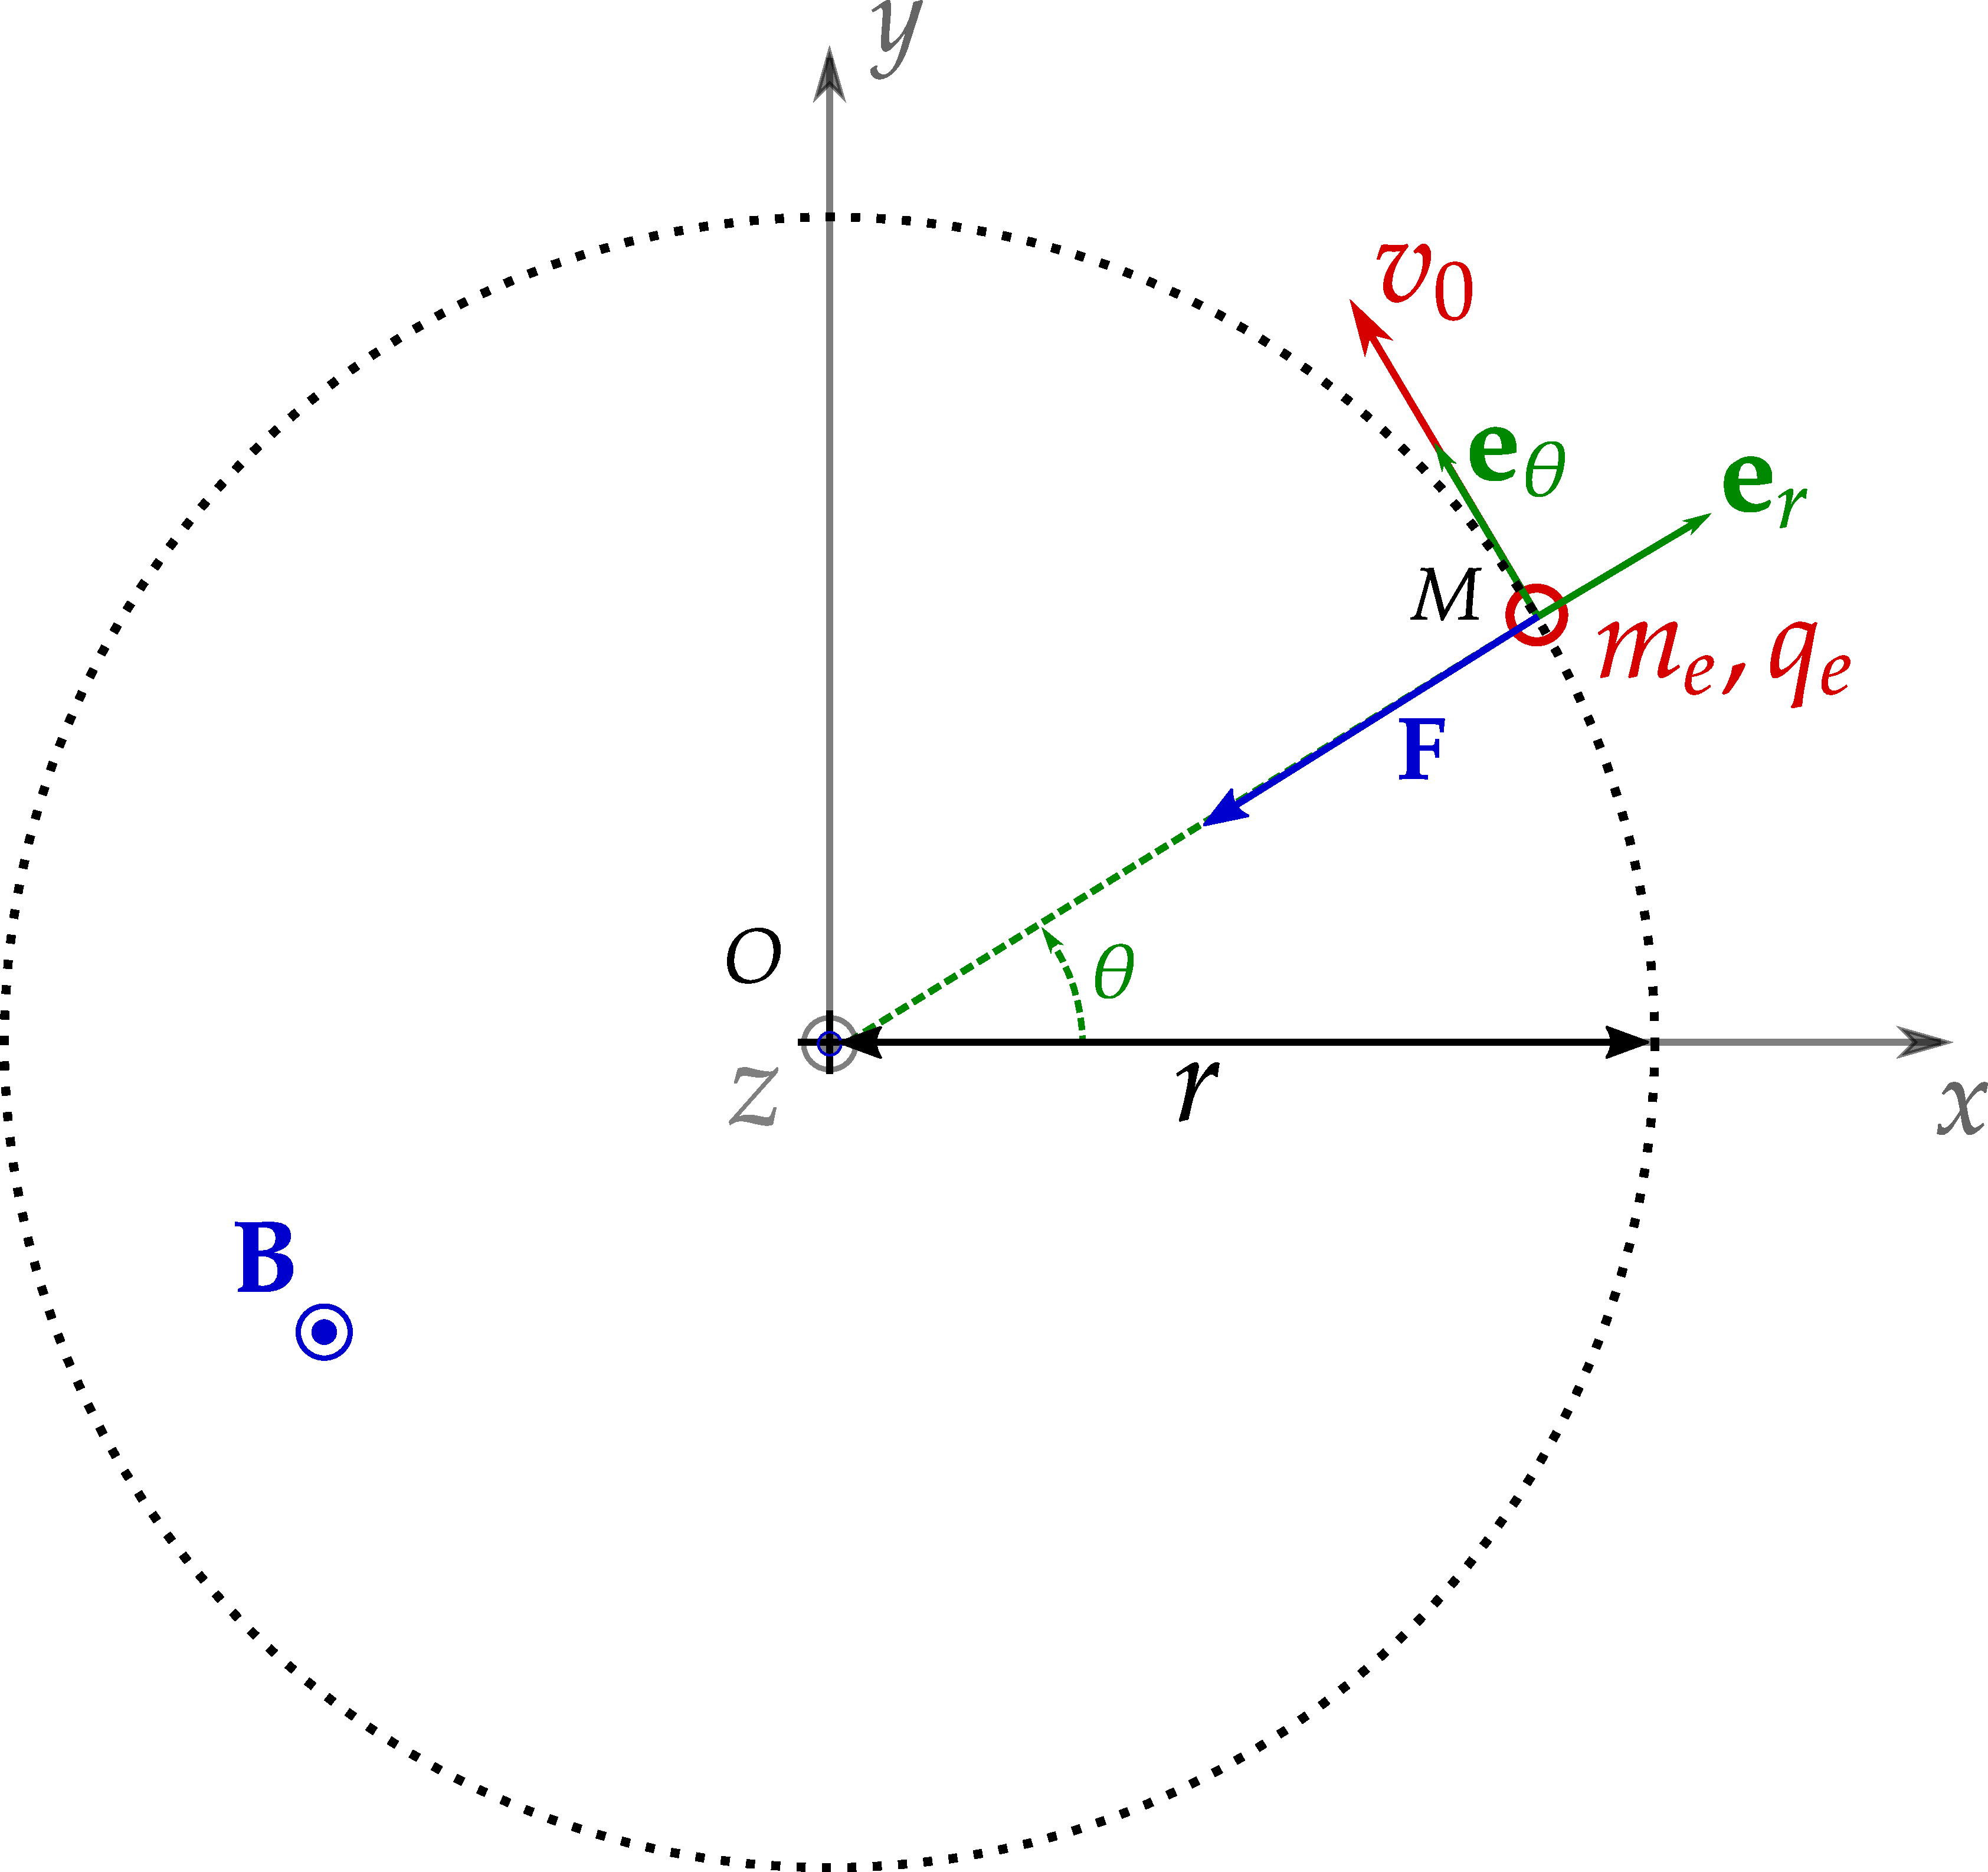
\includegraphics[scale=0.75]{cyclotron}
	\caption{Trajectoire d'un électron dans un champ magnétique uniforme.}%
	\label{fig:magneto_cyclotron}
\end{figure}

\section{La loi de Biot et Savart}
De la même manière que pour le champ électrostatique, nous
commençons par définir le champ magnétique généré par une charge ponctuelle. 
Soit une charge ponctuelle $q$ en un point $P$ de l'espace se déplaçant 
à la vitesse $\vecv$ dans le référentiel du laboratoire. Expérimentalement,
on observe que cette particule génère
en un point $M$ un champ magnétique $\vecb(M)$ tel que

\begin{equation*}
	\vecb(M) = \dfrac{\mu_0 q}{4 \pi} \vecv \wedge \dfrac{\mitbf{PM}}{||PM||^3},
\end{equation*}
où $\mu_0 = \unit{4 \pi \times 10^{-7}}{\tesla \usk \meter \usk \reciprocal 
\ampere}.$

\begin{figure}[h!]
	\centering
	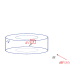
\includegraphics[]{biot_savart}
	\caption{Champ magnétique généré par un élément infinitésimal d'un conducteur
	de densité volumique de courant $\vecj$ en un point $M$ de l'espace.}%
	\label{fig:magneto_biot_savart}
\end{figure}

On considère un conducteur formant un volume $\mathcal{V}$ 
(voir Fig.~\ref{fig:magneto_biot_savart}) parcouru par des charges mobiles 
de densité volumique de charge $\rho$ se déplaçant à la vitesse $\vecv$. Un élément 
infinitésimal $\dV$ de ce circuit centré en $P$ génère en un point $M$ un champ magnétique

\begin{equation*}
	\mathrm{\textbf{d}}\mitbf{B}^P(M) = \dfrac{\mu_0 \rho(P) \dV}
	{4 \pi} \vecv(P) \wedge 
	          \dfrac{\mitbf{PM}}{||PM||^3},
\end{equation*}
où on reconnaît le vecteur densité de courant $\vecj(P) = \rho(P) \vecv(P)$. 
Le champ magnétique
$\vecb$ généré par l'ensemble du circuit en $M$ est alors obtenu en additionnant les 
contributions de chaque élément de ce dernier grâce au principe de superposition
\begin{equation*}
	\vecb(M) = \iiint_{P \in \mathcal{V}} \mathrm{\textbf{d}}\mitbf{B}^P(M)
		 = \iiint_{P \in \mathcal{V}} \dfrac{\mu_0}
		 {4 \pi} \vecj(P) \wedge 
	          \dfrac{\mitbf{PM}}{||PM||^3} \dV
\end{equation*}
On aboutit ainsi à la loi de Biot et Savart.

\begin{defn}[Loi de Biot et Savart]
	Le champ magnétostatique $\vecb(M)$ créé au point $M$ par une distribution
	volumique de courant $\vecj$ ($\ampere \usk \rpsquare \meter$) contenue
	dans un volume $\mathcal{V}$ est
	\begin{equation}
		\vecb(M) = \dfrac{\mu_0}{4 \pi} \iiint_{P \in \mathcal{V}} 
		\dfrac{\vecj(P) \wedge \mitbf{PM}}{||PM||^3} \dV,
	\end{equation}
	où $\mu_0 = \unit{4 \pi \times 10^{-7}}{\tesla \usk \meter \usk \reciprocal
	\ampere}$ est la perméabilité magnétique du vide.

\end{defn}

	Par un raisonnement similaire, on montre que pour une distribution 
	surfacique de courant $\vecj_s$ confinée sur une 
	surface $\mathcal{S}$, cette expression devient
	\begin{equation}
		\vecb(M) = \dfrac{\mu_0}{4 \pi} \iint_{P \in \mathcal{S}} 
		\dfrac{\vecj_s(P) \wedge \mitbf{PM}}{||PM||^3} \mathrm{d}S.
	\end{equation}

	Pour un circuit filiforme $\mathcal{C}$ parcouru par un courant $I$, 
	cette expression devient
	\begin{equation}
		\vecb(M) = \dfrac{\mu_0}{4 \pi} \int_{P \in \mathcal{C}} 
	\dfrac{I \dl \wedge \mitbf{PM}}{||PM||^3}.
	\end{equation}

\begin{exemple}
	On cherche à déterminer le champ magnétique généré par un fil infini $\mathcal{C}$
	parcouru
	par un courant d'intensité $I$ en un point $M$ 
	(voir Fig.~\ref{fig:magneto_spire}). On se place dans un repère cylindrique
	$(0, \er, \etheta, \ez)$. Les points $M$ et $P$ ont pour coordonnées 
	respectives $(r, \theta, 0)$ et $(0, 0, z_P)$.

	Le champ magnétique $\mathrm{\textbf{d}}\vecb^P(M)$ généré par un élément
	$\dl_P$ du fil centré en $P$ s'écrit
	\begin{equation*}
	\mathrm{\textbf{d}}\vecb^P(M) = \dfrac{\mu_0}{4 \pi} 
	              \dfrac{I \dl_P \wedge \mitbf{PM}}{||PM||^3},
	\end{equation*}
	où $\mitbf{PM} = \mitbf{PO} + \mitbf{OM} = - z_P\ez + r\er$. Dans un repère
	cylindrique, un élément infinitésimal $\dl_P$ du fil s'écrit
	$\dl_P = \dz_P \ez$. On a alors
	\begin{equation*}
		\dfrac{\dl_P \wedge \mitbf{PM}}{||PM||^3} = 
		\dfrac{r\dz_P}{||PM||^3}\etheta. 	
	\end{equation*}
	En remarquant que $||PM|| = r/\cos\alpha$, l'expression précédente devient alors
	\begin{equation*}
		\dfrac{r\dz_P}{||PM||^3}\etheta = \dfrac{\cos^3\alpha \dz_P}
		{r^2} \etheta
	\end{equation*}
	De même, on remarque que $z_p = r \tan\alpha$.
	Par différentiation, on obtient donc
	\begin{equation*}
		\dz_P = \mathrm{d}\left[r\tan\alpha\right] = 
		\dfrac{r \mathrm{d}\alpha}{\cos^2\alpha}.
	\end{equation*}
	Finalement,
	\begin{equation*}
		\mathrm{\textbf{d}}\vecb^P(M) = \dfrac{\mu_0 I \cos\alpha}
		{4 \pi r} \mathrm{d}\alpha \etheta.
	\end{equation*}
	Le champ $\vecb(M)$ généré au point $M$ par le fil s'obtient alors
	en utilisant le principe de superposition, ce qui revient à intégrer les champs 
	magnétiques infinitésimaux sur l'ensemble du fil. Pour parcourir l'ensemble du
	fil, $\alpha$ doit varier entre $-\pi/2$ et $\pi/2$. On a alors
	\begin{equation*}
		\boxed{\vecb(M) = \dfrac{\mu_0 I}{4\pi r}
			\times \displaystyle{\int_{-\pi/2}^{\pi/2} 
			\cos\alpha\mathrm{d}\alpha \etheta} =
	\dfrac{\mu_0 I}{2\pi r}\etheta.}
	\end{equation*}
	On obtient un champ magnétique porté par $\etheta$ et donc la norme ne dépend
	que de $r$. Les lignes de ce champ sont des cercles concentriques centrés
	sur le fil. $\vecb$ "tourne" autour du fil.
\end{exemple}
\begin{figure}[h!]
	\centering
	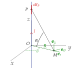
\includegraphics[scale=0.7]{fil}
	\caption{Champ magnétique créé en un point $M$ par un fil parcouru par
	un courant d'intensité $I$.}%
	\label{fig:magneto_spire}
\end{figure}

\begin{defn}[Calcul du champ magnétique par la loi de Biot et Savart]
	Comme nous l'avons vu dans l'exemple précédent, la loi de Biot et Savart
	peut s'avérer utile lorsqu'il s'agit de calculer le champ magnétique 
	$\vecb$ généré par une distribution de courant. Voici en résumé la démarche à suivre
	\begin{enumerate}
		\item Réaliser un schéma du système et choisir un repère adapaté.
		\item Exprimer le petit volume $\dV$, de surface $\mathrm{d}S$
		  ou de longueur $\dl$ dans ce système de coordonnées.
	  \item En multipliant cet élément par le courant ($\vecj$, $\vecj_s$ ou
	    $I$), on obtient le petit élément de courant associé.
	  \item Exprimer le vecteur $\mitbf{PM}$ dans le système de coordonnées
	    choisi.
    	\item En multipliant par $\dfrac{\mu_0}{4 \pi}$ et en faisant le produit 
	  vectoriel par $\dfrac{\mitbf{PM}}{||PM||^3}$, on fabrique le champ
	  élémentaire $\mathrm{\textbf{d}}\vecb^P(M)$ généré en $M$.
	\item Pour calculer $\vecb(M)$, il suffit alors d'intégrer sur la distribution
	  de courant.
	\end{enumerate}
\end{defn}
\section{Équation de la magnétostatique}
On considère un fil parcouru par un courant $I$ dans un
repère cylindrique $(O, \er, \etheta, \ez)$ (voir Fig.~\ref{fig:magneto_spire}). 
Comme vu ci-dessus, le champ
magnétique créé par ce fil en un point $M$ situé à une distance $r$ du fil
est donné par
\begin{equation*}
	\vecb(M) = \dfrac{\mu_0 I}{2 \pi r}\etheta.
\end{equation*}
Comme pour le champ électrostatique, nous allons nous servir de cet exemple simple 
pour retrouver certaines propriétés du champ magnétostatique.

\subsection{Le théorème d'Ampère}
Le théorème d'Ampère est l'équivalent pour le champ magnétostatique $\vecb$
du théorème de Gauss. Il va nous permettre de calculer facilement le champ
magnétostatique généré par une distribution de courants simple.

Les lignes du champ $\vecb$ créé par le fil sont des cercles dont l'axe est le
fil. Nous cherchons donc dans un premier temps à calculer la circulation de $\vecb$ 
sur la ligne de champ $\mathcal{C}$ de rayon $r$ passant par $M$. 
On a bien pris soin au préalable
d'orienter cette dernière. Dans un repère cylindrique, un petit élément $\dl$ de ce 
contour fermé s'écrit $\dl = r \dtheta \etheta$. La circulation de $\vecb$ sur
ce contour s'écrit donc
\begin{equation*}
	\boxed{\displaystyle{\oint_\mathcal{C} \vecb \cdot \dl = 
		\oint_0^{2 \pi} \dfrac{\mu_0 I}{2 \pi r} r\dtheta
	= \mu_0 I.}}
\end{equation*}
On constate que la circulation du champ $\vecb$ le long du circuit $\mathcal{C}$
ne dépend que du courant $I$ que ce dernier enlace. Cette propriété que nous venons
de montrer pour un fil est en fait une propriété générale du champ magnétostatique.

\begin{defn}[Théorème d'Ampère]
	La circulation du champ magnétostatique $\vecb$ le long d'un circuit fermé
	$\mathcal{C}$ est égale au courant \textbf{algébrique} $I_\mathrm{int}$ 
	enlacé par ce dernier multiplié
	par $\mu_0$
	\begin{equation}
		\oint_\mathcal{C} \vecb \cdot \dl = \mu_0 I_\mathrm{int}.
	\end{equation}
	Le contour sur lequel est réalisée l'intégrale est appelé contour d'Ampère.
	Le courant enlacé $I_\mathrm{int}$ est le courant qui traverse une surface 
	orientée
	qui s'appuie sur le contour d'Ampère. L'orientation de la surface 
	se déduit de celle du contour
	grâce à la règle de la main droite ou du tire-bouchon.
\end{defn}

\begin{exemple}
	\begin{minipage}{0.6\linewidth}
	Soit deux fils électriques parcourus par des courants $I_1$ et $I_2$.
	Avec les orientations choisies, le théorème d'Ampère appliqué au 
	contour $\mathcal{C}$ s'écrit
	\begin{equation*}
		\oint_\mathcal{C} \vecb \cdot \dl = \mu_0(I_1 - I_2).
	\end{equation*}
	\end{minipage}
	\hfill
	\begin{minipage}{0.35\linewidth}
		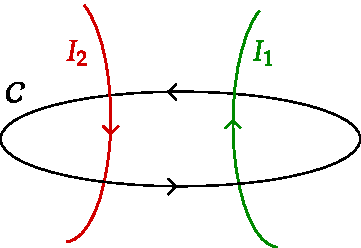
\includegraphics[width=0.8\linewidth]{ampere_ex}
	\end{minipage}

\end{exemple}

Le théorème d'Ampère peut-être traduit sous une forme locale:
appelée \textbf{équation de Maxwell-Ampère}, qui relie alors le champ magnétostatique
au vecteur densité de courant.

\begin{defn}[Équation de Maxwell-Ampère]
	L'équation de Maxwell-Ampère relie le champ magnétostatique $\vecb$
	au vecteur densité de courant $\vecj$
	\begin{equation}
		\rot \vecb = \mu_0 \vecj.
		\label{eq:magneto_ma}
	\end{equation}
	Cette équation est une relation $\textbf{locale}$, elle permet de relier 
	les dérivées spatiales du champ $\vecb$ en un point de l'espace au vecteur
	$\vecj$ en ce même point.
\end{defn}

\subsection{Flux du champ magnétostatique $\vecb$}
On cherche maintenant à calculer la divergence du champ $\vecb$. En coordonnées 
cylindriques, cela donne
\begin{equation*}
	\div \vecb = \dfrac{1}{r}\left(\dd{r B_r}{r} + \dd{B_\theta}{\theta} \right)
	+ \dd{B_z}{z},
\end{equation*}
où $B_r$, $B_\theta$ et $B_z$ sont les composantes de $\vecb$. 
Dans le cas du fil infini, $B_\theta$ est la seule composante non nulle de $\vecb$ 
et elle ne dépend pas
de $\theta$. On a donc
\begin{equation*}
	\div \vecb = 0.
\end{equation*}
Ce résultat se généralise à un champ magnétostatique $\vecb$ quelconque sous
la forme de l'équation de Maxwell-Thomson.

\begin{defn}[Équation de Maxwell-Thomson]
	Un champ magnétique $\vecb$ vérifie toujours
	\begin{equation*}
		\div \vecb = 0.
	\end{equation*}
	Cette relation locale est vérifiée en tout point de l'espace.
\end{defn}

\begin{rem}
La divergence de $\vecb$ étant nulle, l'analyse vectorielle affirme
qu'il est possible dans ce cas de définir un champ vectoriel $\veca$,
défini à un gradient près, tel que $\rot \veca = \vecb$,
appelé le potentiel vecteur.
\end{rem}

Comme l'équation de Maxwell-Ampère, cette équation peut se mettre sous une forme
intégrale, en exprimant le flux du champ magnétique à travers une surface fermée
$\mathcal{S}$.

\begin{defn}[Flux du champ magnétostatique]
	Le flux du champ magnétique $\vecb$ à travers une surface fermée 
	$\mathcal{S}$ est nul
	\begin{equation*}
		\oiint_\mathcal{S} \vecb \cdot \ds = 0.
	\end{equation*}
	On dit que le champ $\vecb$ est à flux conservatif.
\end{defn}

	\begin{minipage}{0.6\linewidth}
	On peut appliquer ce résultat à une surface $\mathcal{S}$ particulière
	constituée d'une portion de tube de champ de section d'entrée $\mathcal{S}_e$,
	de section de sortie $\mathcal{S}_s$ et de section latérale $
	\mathcal{S}_l$. 	
	\end{minipage}
	\hfill
	\begin{minipage}{0.3\linewidth}
	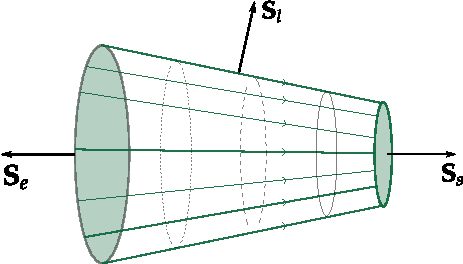
\includegraphics[scale=0.7]{tube}
	\end{minipage}
	\vspace{0.5cm}

\begin{defn}[Tube de champ]
	L'ensemble des lignes de champ s'appuyant sur un contour fermé forme un 
	tube de champ.
\end{defn}
	
	D'après le théorème d'Ampère la flux de $\vecb$ à
	travers cette surface est nul.
	Par définition du tube de champ, l'intégrale sur la surface 
	latérale est nulle. Il reste donc 
	\begin{equation*}
		\iint_\mathcal{S_e} \vecb \cdot \ds_e =
		- \iint_\mathcal{S_s} \vecb \cdot \ds_s 
		\iff
		\displaystyle{\left\lvert\iint_\mathcal{S_e} \vecb \cdot \ds_e\right\rvert =
		\left\lvert\iint_\mathcal{S_s} \vecb \cdot \ds_s\right\rvert}.
	\end{equation*}
	Le flux entrant dans la surface est égal au flux sortant de cette dernière.
	De plus, la surface de sortie étant de taille plus importante que 
	la surface d'entrée, on en conclut que le champ est plus intense
	à l'entrée du tube qu'à la sortie. Le champ $\vecb$ étant à flux
	conservatif, un resserrement des lignes de champs traduit une augmentation
	de l'intensité de ce dernier.

\begin{defn}[Flux conservatif et lignes de champ]
	Le champ magnétique étant à flux conservatif, ses lignes de champs
	se resserrent dans les zones de forte intensité. Inversement, ces dernières
	s'éloignent lorsqu'il devient plus faible
\end{defn}

\section{Étude des lignes de champ de \vecb}
Nous nous intéressons dans cette partie aux propriétés spatiales du champ $\vecb$.
Nous allons voir comment les \textbf{lignes de champ} nous renseignent sur sa répartition 
dans l'espace.

Nous nous intéressons au champ magnétique produit par un solénoïde 
(voir Fig.~\ref{fig:magneto_solenoide}).
Les lignes de champ nous permettent de retrouver quelques propriétés du champ 
magnétostatique énoncées précédemment.

\begin{figure}[htpb]
	\centering
	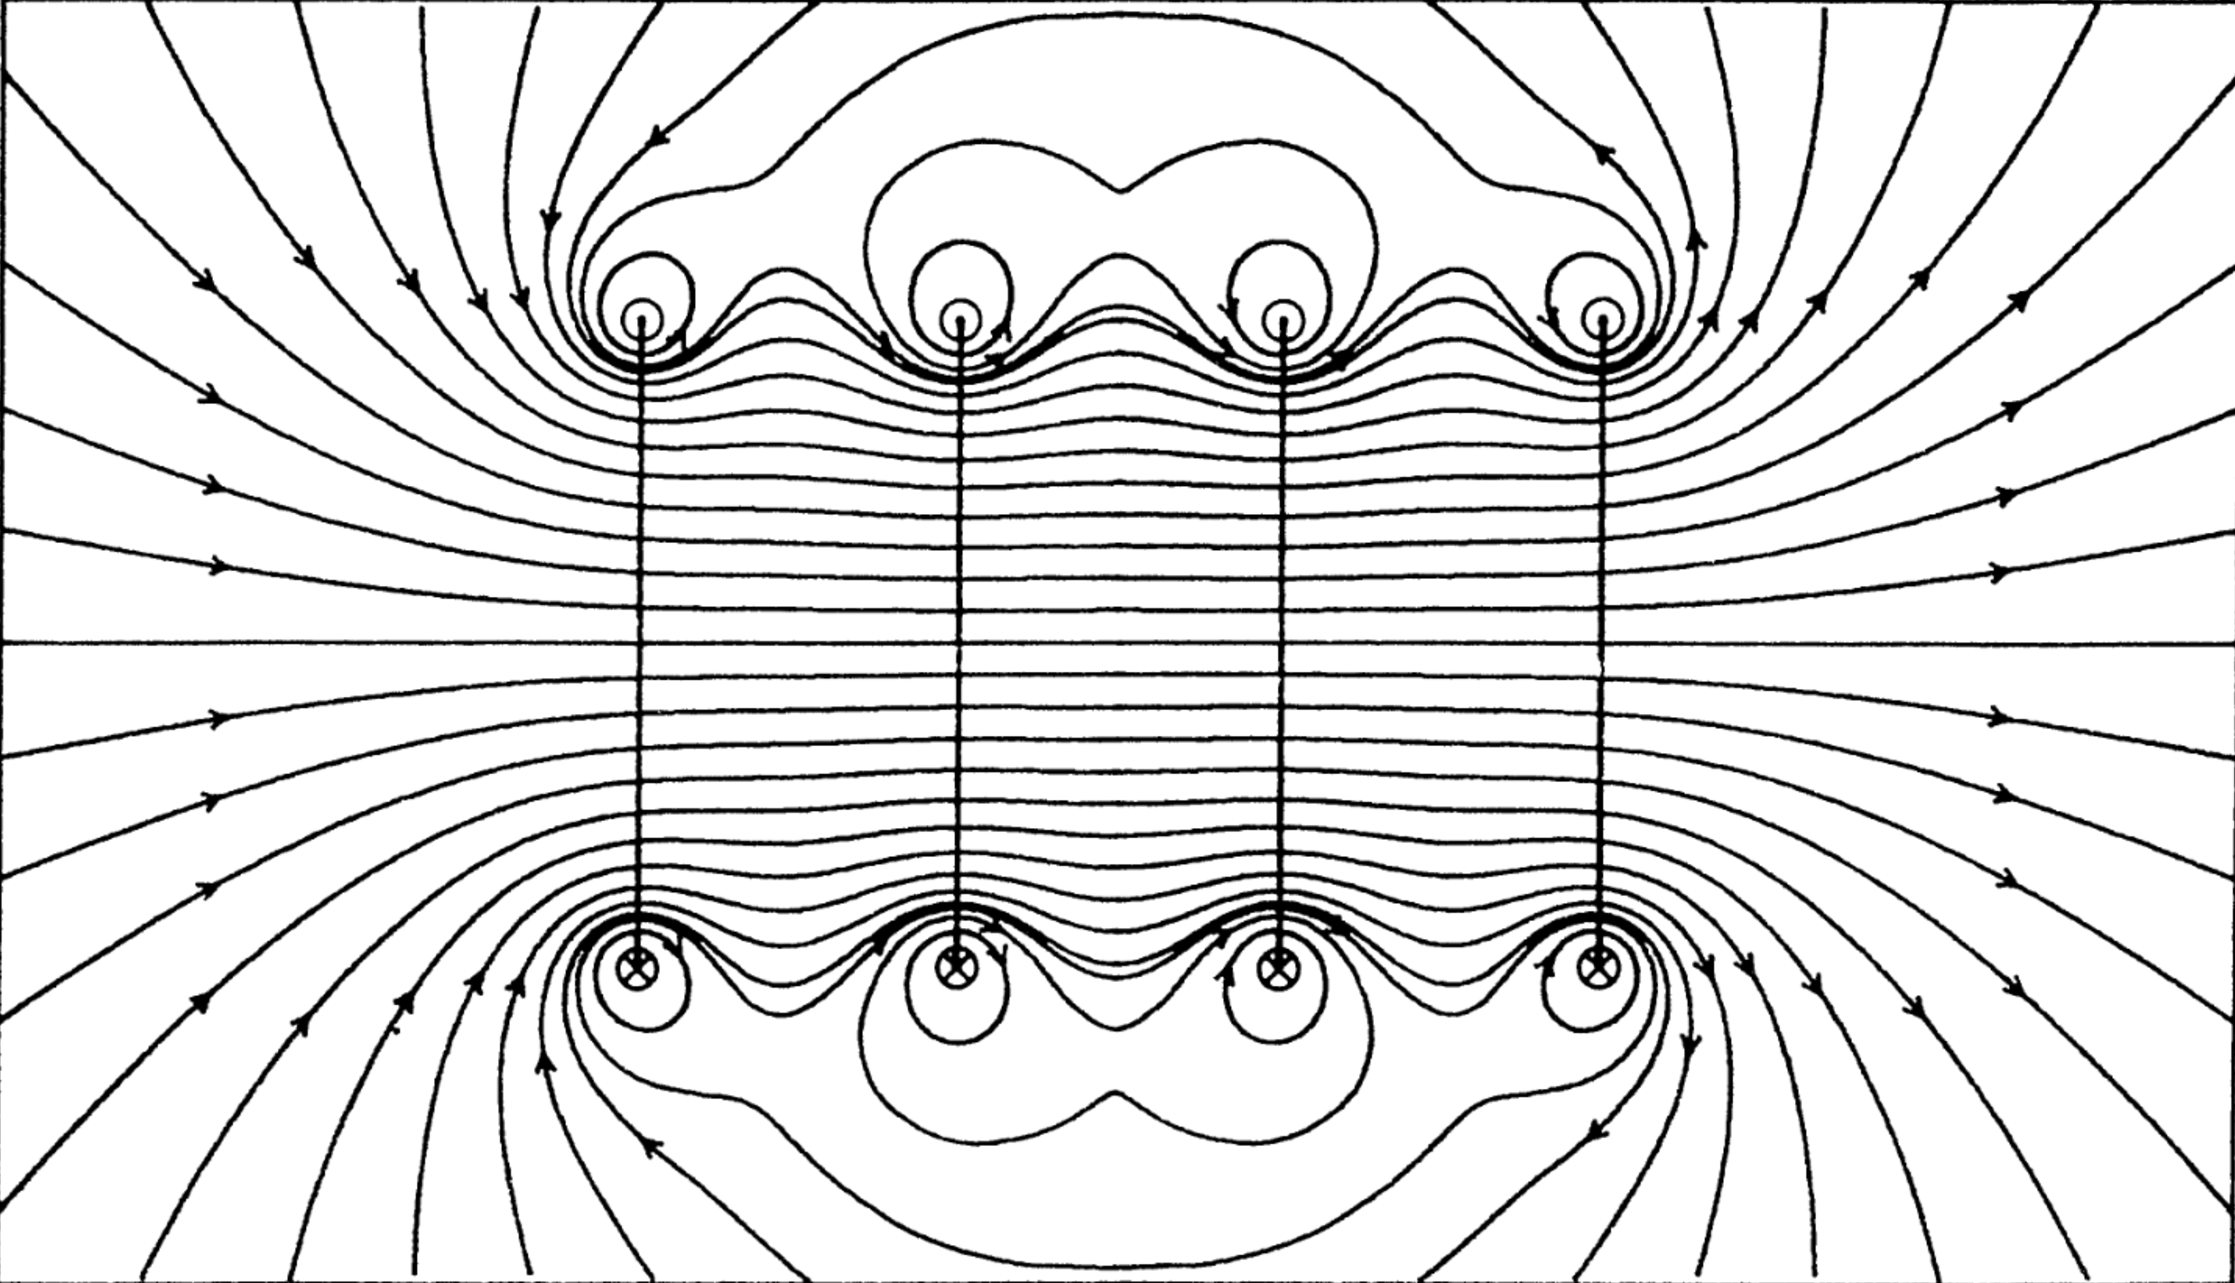
\includegraphics[width=0.7\linewidth]{solenoide}
	\caption{Lignes du champ magnétique généré par un solénoïde constitué de
		4 bobines parcourues dans le même sens par la même intensité.
		Cette figure est extraite de \cite{Gie1985}}%
	\label{fig:magneto_solenoide}
\end{figure}

\begin{enumerate}
	\item On remarque tout d'abord que les lignes de champ 
	  sont des contours fermés qui entourent les fils parcourus par un courant.
	  Cette première observation est une conséquence directe de l'équation
	  de Maxwell-Ampère. L'orientation de ces lignes de champ s'obtient
	  d'ailleurs en considérant le sens du courant dans les fils et en utilisant
	  la règle de la main droite.
      \item La divergence nulle de $\vecb$ est aussi visible sur cette carte de 
	champ. En effet, on constate que les lignes de champ ne convergent/divergent
	pas en un point de l'espace, contrairement au champ électrostatique.
      \item Dans le cas du champ magnétique, le resserrement des lignes de champ
	traduit une augmentation de la norme de ce dernier. On conclut que le champ
	est plus intense à l'intérieur du solénoïde qu'à l'extérieur. De plus, les
	lignes de champ étant parallèles à l'intérieur du solénoïde, on conclut que
	le champ est uniforme.
      \item Grâce aux lignes de champ, on retrouve rapidement les plans de 
	  symétrie et d'antisymétrie du champ magnétique. Le plan médiateur 
	  du solénoïde est par exemple un plan de symétrie du champ magnétique. 
          L'analyse de ces symétries sera utile pour calculer le champ
          magnétique résultant d'une distribution de courant.
\end{enumerate}

\section{Calcul du champ magnétostatique}
\label{sec:calcul_e}
Nous allons voir dans cette partie comment nous pouvons utiliser le théorème d'Ampère
pour calculer le champ magnétostatique $\vecb$ créé 
par une distribution de courants simple. Nous nous intéressons ici à une bobine
torique constituée d'un fil régulièrement bobiné autour d'un tore de section
carré (voir Fig.~\ref{fig:magneto_tore}). Cette bobine est caractérisée par le nombre $N$
total de spires bobinés, son rayon intérieur $R$ 
et sa hauteur $h$. La bobine est parcourue par un courant $I$.

On cherche à déterminer 
l'expression du champ électrique $\vecb$ en un point $M$ de l'espace. Pour ce faire, 
il suffit de suivre le mode d'emploi suivant
\begin{enumerate}
	\item Faire un schéma du système ! C'est absolument indispensable
	  (voir Fig.~\ref{fig:magneto_tore})
	\item Choisir un repère adapté au problème
	\item Étudier les invariances de cette distribution
	\item Étudier les symétries de la distribution de courants à l'origine 
	  du champ magnétostatique
	\item Choisir un contour d'Ampère et appliquer le théorème d'Ampère.
\end{enumerate}

Au vu de la géométrie du système, nous choisissons ici d'utiliser 
un repère cylindrique $(O, \er, \etheta, \ez)$.
Le point $M$ est donc repéré par ses coordonnées $(r, \theta, z)$. Le champ
magnétostatique en $M$ s'écrit de manière générale

\begin{equation}
	\vecb(M) = B_r(M)\er + B_\theta(M)\etheta + B_\varphi(M)\ephi.
	\label{eq:tore}
\end{equation}
Le champ magnétostatique est un vecteur à trois composantes et chaque composante
dépend des coordonnées de $M$. Pour simplifier cette expression, il est intéressant
de considérer les invariances et symétries de la distribution de courant qui génère
le champ $\vecb$.

\begin{figure}
	\centering
	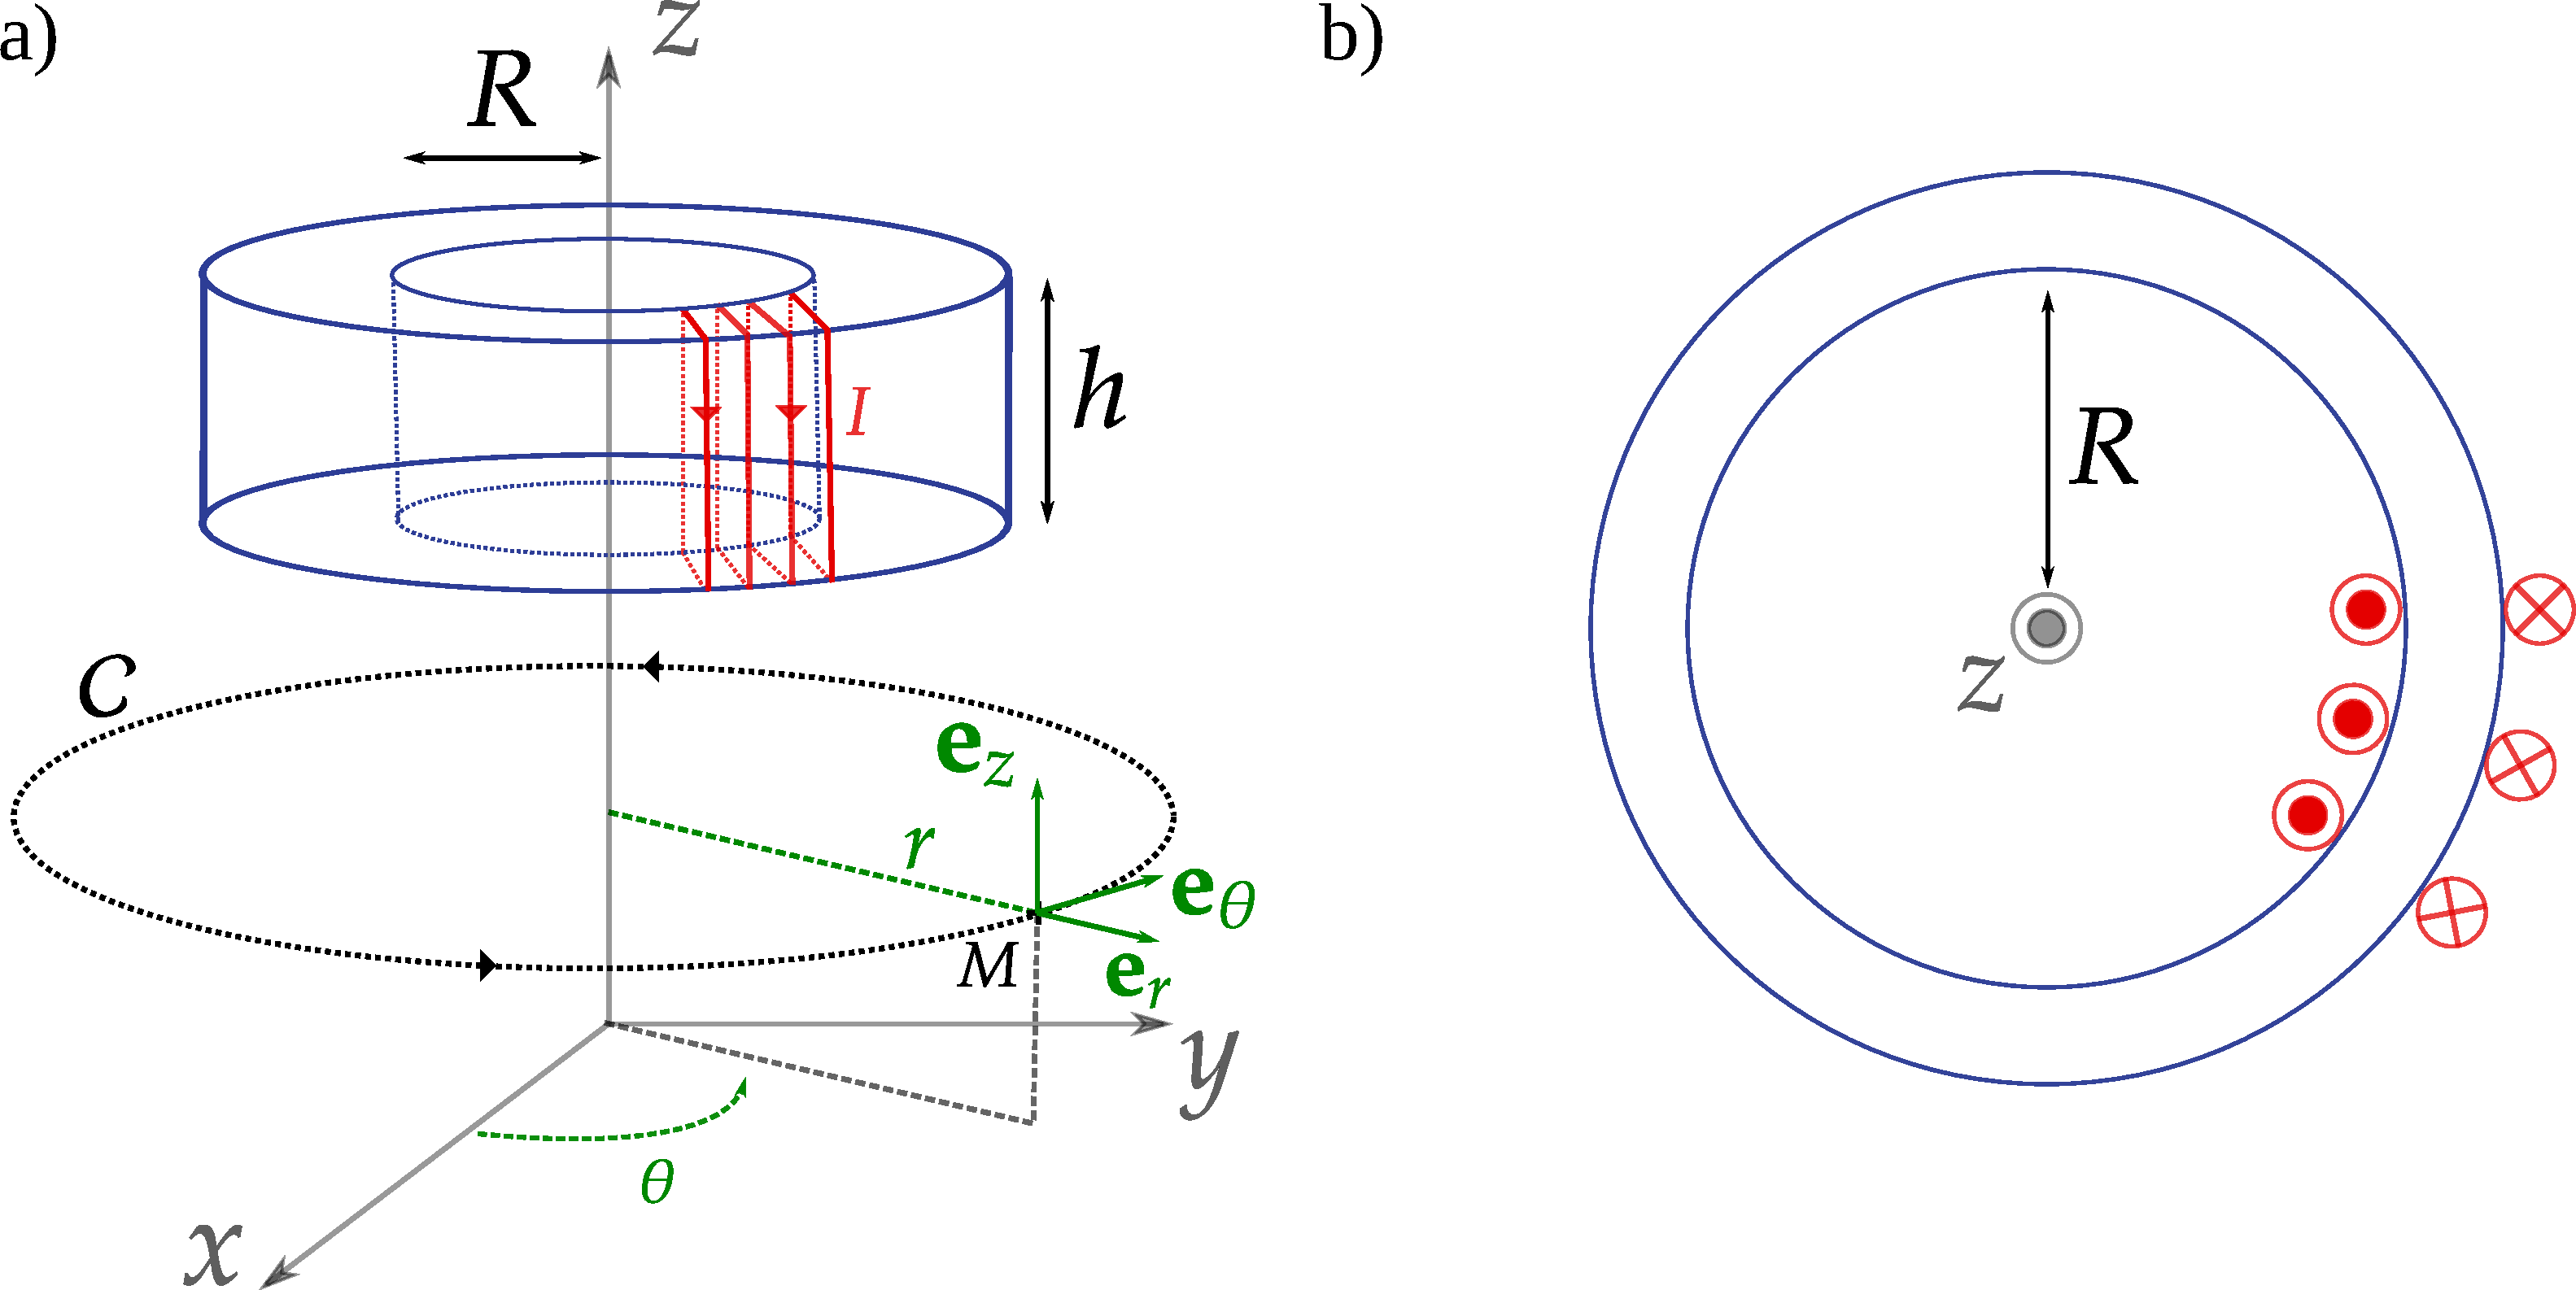
\includegraphics[scale=1]{tore}
	\caption{Bobine torique à gauche et coupe perpendiculaire à $(Oz)$
	de cette bobine à droite.}%
	\label{fig:magneto_tore}
\end{figure}

\subsection{Invariance de la distribution de courants}
On cherche ici à savoir si la distribution de courant est modifiée sous l'effet
d'une translation ou d'une rotation de l'espace. En d'autres termes, on regarde
de quelles variables elle dépend. Étant donné que les spires sont uniformément
répartie sur le tore, on observe que

\begin{itemize}
	\item  si je tourne le tore d'un angle $\Delta \theta$ dans la
	  direction $\etheta$, le problème
	  ne change pas. La distribution de courant est donc invariante 
	  par rotation selon l'angle $\theta$. $\vecb$ \textbf{ne dépend pas de
	  $\mitbf{\theta}$}.
\end{itemize}

Finalement, l'expression~\ref{eq:tore} du champ magnétique se simplifie donc en 

\begin{equation*}
	\boxed{\vecb(M) = B_r(r,z)\er + B_\theta(r,z)\etheta + B_z(r,z)\ez.}
\end{equation*}
\subsection{Symétries de la distribution de courants}

Si on applique ce principe au champ magnétique créé par une distribution 
de courants, cela revient à dire que les symétries de la distributions de 
courants doivent se retrouver dans les symétries du champ magnétique. On en 
déduit les règles suivantes

\begin{defn}[Symétries de $\vecb$ et de la distribution de courant]
\begin{itemize}
  \item si $(\Pi)$ est un plan d'antisymétrie de la distribution de courant et que 
    $M$ appartient à $(\Pi)$, alors obligatoirement $\vecb(M)$ doit 
    appartenir à $(\Pi)$,
  \item si $(\Pi)$ est un plan de symétrie de la distribution de courant 
    et que $M$ appartient à $(\Pi)$, alors obligatoirement $\vecb(M)$ doit 
    être orthogonal à $(\Pi)$.
\end{itemize}
\end{defn}

\begin{rem}
	Le champ magnétostatique $\vecb$ appartient aux plans d'\textbf{antisymétrie}
	de la distribution de courant et non aux plans de symétrie comme
	c'est le cas pour le champ électrostatique. Le vecteur $\vecb$ est 
	qualifié de vecteur axial.
\end{rem}

Pour appliquer ces règles à notre exemple, on détermine les plans de symétrie 
et d'antisymétrie de la distribution de courants auquels 
le point $M$ appartient

\begin{itemize}
	\item le plan $(M, \er, \ez)$ est un plan de symétrie de la distribution
	  de courant. $\vecb(M)$ \textbf{doit être orthogonal à ce plan}.
\end{itemize}

$\vecb(M)$ doit être orthogonal au plan $(M, \er, \ez)$, 
il doit donc être colinéaire à $\etheta$

\begin{framed}
\begin{equation*}
	\vecb(M) = B_\theta(r, z) \etheta.
\end{equation*}
\end{framed}

Nous n'avons imposé aucune condition sur la position de $M$, cette relation est
donc vraie pour tout point $M$ de l'espace. Maintenant que l'expression du 
champ magnétique a été simplifiée au maximum, on cherche à appliquer le théorème
d'Ampère.

\subsection{Application du théorème d'Ampère}
La distribution de courant présente une symétrie de révolution. On choisit comme contour 
d'Ampère un cercle $\mathcal{C}$ de rayon $r$, de centre $O$ et orienté
dans le sens de $\etheta$ qui passe par $M$ 
(voir Fig~\ref{fig:magneto_tore}) et on applique le théorème d'Ampère à ce dernier

\begin{equation*}
	\oint_\mathcal{S} \vecb(M) \cdot \dl = \mu_0 I_\mathrm{int},
	\label{eq:cavite_gauss}
\end{equation*}
où $I_\mathrm{int}$ est la courant enlacé par $\mathcal{C}$. On commence
par déterminer l'expression du membre de gauche. Dans un repère cylindrique,

\begin{equation*}
	\dl = r \dtheta \etheta.
\end{equation*}
On obtient alors
\begin{equation*}
	\oint_\mathcal{C} \vecb(M) \cdot \dl = 
	\oint_\mathcal{C} B(r,z) \etheta \cdot r \dtheta \etheta
	= B(r, z) r \int_0^{2 \pi} \dtheta
	= 2 \pi r B(r,z).
\end{equation*}
On s'intéresse maintenant au terme de droite de l'équation.
Deux cas de figure se présentent:
\begin{itemize}
	\item $M$ est situé dans le tore: le courant enlancé par $\mathcal{C}$ est alors
	  $I_\mathrm{int} = NI$.
       \item $M$ est situé à l'extérieur du tore: le courant enlacé par 
	       $\mathcal{C}$ est donc nul. Soit parce que le contour n'enlace 
	       aucun courant, soit parce qu'il enlace autant de courants positifs
	       que de courants négatifs.
\end{itemize}
Finalement,
\begin{framed}
\begin{itemize}
	\item si $M$ se trouve à l'intérieur du tore, 
	  $\vecb(M) = \dfrac{\mu_0 N I}{2 \pi r} \etheta$.
	\vspace{1em}
\item si $M$ est en dehors du tore, $\vecb(M) = \mitbf{0}$. 
\end{itemize}
\end{framed}
%\nocite{*}
%\putbib[magnetostatique]

%\newpage

%\input{exercices/magnetostatique}



